%-----------------------Inicio Preámbulo-----------------------------------------------
\documentclass[letterpaper,12pt]{thesis}
\raggedbottom
\usepackage{layout}
\usepackage[utf8]{inputenc}
\usepackage[pdftex]{graphicx}
\usepackage{tikz}
\usepackage{titlesec}
\usepackage{parskip}
\usepackage{amsfonts,amsmath,amssymb,amsthm,mathrsfs}
\usepackage{latexsym,wasysym}
%manejando los margenes
\usepackage[letterpaper, textwidth=5.94095 in, textheight=21.3 cm, footskip = 0.815cm, left=1.5748 in, top=1.55480315in,twoside ]{geometry}
%\usepackage[paper=letterpaper, marginparsep=0in,footskip = 0.7505cm, marginparwidth= 0in, headsep= 0in, headheight= 0in, top=4cm, bottom=2.5cm,left=4cm,right=2.5cm,twoside]{geometry}
\usepackage{textcomp}
\usepackage[all]{xy}
\usepackage{longtable}
\usepackage[spanish]{babel}
\addto\captionsspanish{\renewcommand{\listfigurename}{ÍNDICE DE ILUSTRACIONES}}
\usepackage{bibthesis,color, enumerate, indentfirst}
\usepackage{hyperref,url,breakurl}
\usepackage{ dsfont }
%para manejar las imagenes (titulos y subtitulos de)
\usepackage{caption}
\usepackage{subcaption}
%para cambiar letra de subcaption a 10 pt
\usepackage{etoolbox}
\usepackage[nodisplayskipstretch]{setspace}
%Paquete para el manejo del Indice
\usepackage[titles]{tocloft}




%---------------------------Fin Preambulo------------------------------------------------
%------------Nueva Definicion para ámbito proof.
\makeatletter
\newenvironment{proof*}[1][\proofname]{\par
  \pushQED{\qed}%
  \normalfont \partopsep=\z@skip \topsep=\z@skip
  \trivlist
  \item[\hskip\labelsep
        \itshape
    #1\@addpunct{.}]\ignorespaces
}{%
  \popQED\endtrivlist\@endpefalse
}
\makeatother


\makeatletter
\g@addto@macro\normalsize{%
  \setlength\abovedisplayskip{1.81em}
  \setlength\belowdisplayskip{1.81em}
  \setlength\abovedisplayshortskip{1.81em}
  \setlength\belowdisplayshortskip{1.81em}
}
%-------------Implementacion distancia titulos, subtitulos, etc -------------
\titlespacing{\section}{0pt}{*0.1}{*0.1} % <------  Separación ente el titulo de seccion y parrafo y seccion y titulo.
\titlespacing{\subsection}{1.76cm}{*0.1}{*0.1} % <------  Separación ente el subtitulo y el inicio de párrafo.



%------------Sección de comandos-----------
\decimalpoint %<--------- para manejar punto decimal en lugar de coma decimal
\setlength{\parindent}{1cm}%<-------------------------sangría
%\setlength{\parskip}{7mm}
\setlength{\parskip}{1.37\baselineskip}%<---------------distancia entre párrafos
\setstretch{1.45}    
%\renewcommand\baselinestretch{1.5}               %<-----------------interlineado
\setlength\LTleft{0pt} \setlength\LTright{0pt} %<------------- parametros para tablas largas








% -------- Modificaciones a Citas (sistema lancasteriano) y direcciones web -------------
\bibpunct[--]{[}{]}{,}{n}{,}{;}
\setlength{\bibsep}{21pt}               % distancia entre items en la bibliograf�a
%\urlstyle{rm}                          % fuente en direcciones web

% ---- Sección de parametrización del Indice General y de ilustraciones -----------------
%Agregar lineas punteadas del capitulo al numero de pagina
\renewcommand{\cftchapleader}{\cftdotfill{\cftchapdotsep}}
\renewcommand{\cftchapdotsep}{\cftdotsep}
%quitar las negrillas para los titulos de los capitulos
\renewcommand{\cftchapfont}{\normalfont}
\renewcommand{\cftchappagefont}{\normalfont}
%Espacio vertical entre capítulos
\setlength{\cftbeforechapskip}{-.01cm}
%Espacio vertical entre secciones y capítulo
\setlength{\cftbeforesecskip}{-0.01cm}
%Espacio vertical entre subsecciones y secciones
\setlength{\cftbeforesubsecskip}{-.01cm}
%Espacio vertical entre subsubsecciones y subsecciones
\setlength{\cftbeforesubsubsecskip}{-.01cm}
% Espacio vertical entre figuras
\setlength{\cftbeforefigskip}{-.01cm}
% Espacio vertical entre tablas
\setlength{\cftbeforetabskip}{-.01cm}
% Espacio del margen al capítulo
\setlength{\cftchapindent}{0cm}
% Espacio entre número y capítulo
\setlength{\cftchapnumwidth}{1.36cm}
% Espacio del margen a la sección
\setlength{\cftsecindent}{1.21cm}
% Espacio entre número y sección
\setlength{\cftsecnumwidth}{1.27cm}
% Espacio del margen a la subsección
\setlength{\cftsubsecindent}{2.93cm}
% Espacio entre número y la subsección
\setlength{\cftsubsecnumwidth}{1.48cm }
% Espacio del margen a la subsección
\setlength{\cftsubsubsecindent}{4.92cm}
% Espacio entre número y la subsubsección
\setlength{\cftsubsubsecnumwidth}{2.25cm}
% Espacio entre número y figura
\setlength{\cftfignumwidth}{1.3cm}
% Espacio del margen a la figura
\setlength{\cftfigindent}{0cm}
% Espacio entre número y tabla
\setlength{\cfttabnumwidth}{1.3cm}
% Espacio del margen a la tabla
\setlength{\cfttabindent}{0cm}
%Para alinear los numeros romanos
\cftsetpnumwidth{2em}


%----------------Definicion de listas----------
%Para listados enumerados
\newcounter{ContadorLista}
\newenvironment{bulletList}{
\begin{list}
{\centering\arabic{ContadorLista}.}
{
\usecounter{ContadorLista}
\setlength{\labelsep}{1.125cm}% Separación entre número y texto
\setlength{\labelwidth}{1cm}
\setlength\listparindent{0cm}
\setlength\leftmargin{1.4cm} % Distancia entre borde y número
\setlength{\parsep}{.0cm}% Separación entre elementos
}
}{
\end{list}
}

%-----------------Definicion de estilos para los teoremas--------------------------------
\newtheoremstyle{ejem} %
  {\baselineskip} % Space above
  {\topsep} % Space below
  {} % Body font
  {} % Indent amount
  {\bfseries} % Theorem head font
  {.} % Punctuation after theorem head
  {.5em} % Space after theorem head
  {} % Theorem head spec (can be left empty, meaning `normal')
\newtheoremstyle{resto} %
  {\baselineskip} % Space above
  {0mm} % Space below
  {\itshape} % Body font
  {} % Indent amount
  {\bfseries} % Theorem head font
  {.} % Punctuation after theorem head
  {.5em} % Space after theorem head
  {} % Theorem head spec (can be left empty, meaning `normal')
  
\theoremstyle{resto}\newtheorem{teorema}{Teorema}[section]
\theoremstyle{resto}\newtheorem{lema}{Lema}[section]
\theoremstyle{resto}\newtheorem{proposicion}{Proposición}[section]
\theoremstyle{resto}\newtheorem{propiedad}{Propiedad}[section]
\theoremstyle{resto}\newtheorem{corolario}{Corolario}[section]
\theoremstyle{ejem}\newtheorem{nota}{Nota}[section]
\newtheorem{solucion}{Solución}[section]
\newtheorem{problema}{Problema}[section]
\theoremstyle{ejem}\newtheorem{definicion}{Definición}[section]
\theoremstyle{ejem}\newtheorem{notacion}{Notación}[section]
\theoremstyle{ejem}\newtheorem{consideracion}{Consideración}[section]
\theoremstyle{ejem}\newtheorem{ejercicio}{Ejercicio}[section]
\theoremstyle{ejem} \newtheorem{ejemplo}{Ejemplo}[section]
\numberwithin{equation}{chapter}
\renewcommand{\theequation}{\thechapter.\arabic{equation}}
%para manejar el estilo de los ejemplos

%---------------- Operadores y funciones -------------------------------------------
\DeclareMathOperator{\car}{car}
\DeclareMathOperator{\rango}{rango}
\DeclareMathOperator{\sop}{sop}
\DeclareMathOperator{\Ima}{Im}
\DeclareMathOperator{\tr}{tr}
\DeclareMathOperator{\grado}{deg}
\makeatother
\newcommand{\srg}[3]{\sum_{#1 \in #2} #3_{#1} #1 }
\newcommand{\modulo}[1]{R\mbox{-módulo}}
\newcommand{\newItem}{\item[$\bullet$]}

%-------palabras claves para el documento --------------------------
\hypersetup{pdftitle = {tituloDePDF}, pdfkeywords = {poner un listado de palabras clave}, pdfauthor = {\textcopyright\ 2012, Hugo Allan García Monterrosa (hugoallangm@gmail.com)}, pdfsubject = {Trabajo
de graduación para obtener la Licenciatura en Matemática Aplicada},
pdfstartview = {FitH}, plainpages = {false}, bookmarksnumbered =
{true}}


\begin{document}
\captionsetup[figure]{labelformat=simple, labelsep=period}


\newpage
\thispagestyle{empty}
%%%%%%%%%%%%%%%%%%%%%%%%%%%%%%%%%%%%%%%%%%%%%%%%%%%%%%%%%%%%%%%%%%%%%%%%%%%%%%%%%%%
%                          Primera Página
%%%%%%%%%%%%%%%%%%%%%%%%%%%%%%%%%%%%%%%%%%%%%%%%%%%%%%%%%%%%%%%%%%%%%%%%%%%%%%%%%%%
%manejando los margenes para que la portada cuadre poner 
\newgeometry{letterpaper, textwidth=5.94095 in, textheight=21.5 cm, footskip = 0.815cm, left=1.5748 in, top=1.55480315in,twoside}
\setbox0\vbox{\noindent
\hspace{.7cm}

\includegraphics[width=2.2cm]{Pictures/escudo.png}}
\ht0=13pt\box0
\hangindent=35mm\hangafter=-3\vspace{-1.72cm}
% aquí está el ecabezado
\noindent Universidad de San Carlos de Guatemala\\
Facultad de Ingeniería\\
Escuela de \Esc  \\ 
\vspace{4.8cm}
\begin{center}
% Título
{\large\textbf{TEORÍA DE LOS GRUPO-ANILLOS}} \\
{\large\textbf{Y SUS APLICACIONES}} \\ 
\vspace{6.50cm}
% Autor
\textbf{\Nomb}\\ 
Asesorado por el \Ases \\
{\centering Lic. William Roberto Gutiérrez Herrera}
\vfill
% Lugar y fecha
Guatemala,  \Fec
\end{center}


\newpage
\thispagestyle{empty}
\mbox{}
\newpage
\thispagestyle{empty}
%%%%%%%%%%%%%%%%%%%%%%%%%%%%%%%%%%%%%%%%%%%%%%%%%%%%%%%%%%%%%%%%%%%%%%%%%%%%%%%%%%%
%                          Segunda Página
%%%%%%%%%%%%%%%%%%%%%%%%%%%%%%%%%%%%%%%%%%%%%%%%%%%%%%%%%%%%%%%%%%%%%%%%%%%%%%%%%%%
\restoregeometry
\begin{center}
UNIVERSIDAD DE SAN CARLOS DE GUATEMALA \\[3mm]

\includegraphics[width=4cm]{Pictures/escudo.png} \\ [1mm]
FACULTAD DE INGENIERÍA\\
\vspace{1.4cm}
{\large\textbf{TEORÍA DE LOS GRUPO-ANILLOS}}\\
{\large\textbf{Y SUS APLICACIONES}} 
\vskip -1em
TRABAJO DE GRADUACIÓN 
\vskip -0.5em
PRESENTADO A LA JUNTA DIRECTIVA DE LA \\ 
FACULTAD DE INGENIERÍA \\ 
POR\\
\vspace{1.4cm}
\textbf{\MakeUppercase{\Nomb}} \\
ASESORADO POR \MakeUppercase{\Ases}\\
{\centering LIC. WILLIAM ROBERTO GUTIÉRREZ HERRERA} 
\vskip -.7em 	
AL CONFERÍRSELE EL TÍTULO DE 
\vskip -.7em
\textbf{\MakeUppercase{\Grado}} \\ 
%\vspace{1.3cm}
\vfill
GUATEMALA, \MakeUppercase{\Fec}
\end{center}

\newpage
\thispagestyle{empty}
\mbox{}
\newpage
\thispagestyle{empty}
%%%%%%%%%%%%%%%%%%%%%%%%%%%%%%%%%%%%%%%%%%%%%%%%%%%%%%%%%%%%%%%%%%%%%%%%%%%%%%%%%%%
%                          Tercera Página
%%%%%%%%%%%%%%%%%%%%%%%%%%%%%%%%%%%%%%%%%%%%%%%%%%%%%%%%%%%%%%%%%%%%%%%%%%%%%%%%%%%

\begin{center}

UNIVERSIDAD DE SAN CARLOS DE GUATEMALA \\
FACULTAD DE INGENIERÍA 


\includegraphics[width=4cm]{Pictures/escudo.png}\\ [17mm]
\vskip -.80em 
\textbf{NÓMINA DE JUNTA DIRECTIVA} 	

\begin{flushleft}
 \begin{tabular}{lll}\vspace{-.04cm}
    &\hspace{1.75cm}DECANO     & \hspace{.355cm} \Dec \\ \vspace{-.04cm}
    &\hspace{1.75cm}VOCAL I    & \hspace{.355cm} \VocI \\ \vspace{-.04cm}
    &\hspace{1.75cm}VOCAL II   & \hspace{.355cm} \VocII \\ \vspace{-.04cm}
    &\hspace{1.75cm}VOCAL III  & \hspace{.355cm} \VocIII \\ \vspace{-.04cm}
    &\hspace{1.75cm}VOCAL IV   & \hspace{.355cm} \VocIV \\ \vspace{-.04cm}
    &\hspace{1.75cm}VOCAL V    & \hspace{.355cm} \VocV \\ \vspace{-.04cm}
    &\hspace{1.76cm}SECRETARIO & \hspace{.354cm} \Sec  
\end{tabular}
\end{flushleft}
\vspace{.8cm}
\textbf{TRIBUNAL QUE PRACTICÓ EL EXAMEN GENERAL PRIVADO} 

\vspace{-.2cm}
\begin{flushleft}
\begin{tabular}{lll}\vspace{-.04cm}
    &\hspace{1.61cm} DECANO     & \hspace{.25cm}\Dec \\ \vspace{-.04cm}
    &\hspace{1.61cm} EXAMINADOR & \hspace{.25cm}\ExaI \\\vspace{-.04cm}
    &\hspace{1.61cm} EXAMINADOR & \hspace{.25cm}\ExaII \\\vspace{-.04cm}
    &\hspace{1.61cm} EXAMINADOR & \hspace{.25cm}\ExaIII \\\vspace{-.04cm}
    &\hspace{1.62cm} SECRETARIO & \hspace{.24cm}\Sec
\end{tabular}
\end{flushleft}
\end{center}

\newpage
\thispagestyle{empty}
\mbox{}
\newpage
\thispagestyle{empty}
%%%%%%%%%%%%%%%%%%%%%%%%%%%%%%%%%%%%%%%%%%%%%%%%%%%%%%%%%%%%%%%%%%%%%%%%%%%%%%%%%%%
%                          Cuarta Página
%%%%%%%%%%%%%%%%%%%%%%%%%%%%%%%%%%%%%%%%%%%%%%%%%%%%%%%%%%%%%%%%%%%%%%%%%%%%%%%%%%%
\begin{center}
{\large\textbf{HONORABLE TRIBUNAL EXAMINADOR}}
\end{center} 
\vspace{1.34cm}
En cumplimiento con los preceptos que establece la ley de la Universidad de
\mbox{San Carlos de Guatemala}, presento a su consideración mi trabajo de
graduación titulado: 
\vspace{1.1cm}
\begin{center}{\large\textbf{TEORÍA DE LOS GRUPO-ANILLOS}} \\
{\large\textbf{Y SUS APLICACIONES}} \\  
\end{center}
\vspace{1.2cm}
Tema que me fuera asignado por la Dirección de la Escuela de \Esc , con fecha \FecP. 
\vspace{0.2cm}
\begin{figure}[!ht]
\begin{flushright}
\begin{tabular}{c}

\includegraphics[scale=1]{Pictures/firma.jpg}\\
\textbf{\Nomb}
\end{tabular}
\end{flushright}
\end{figure}
\newpage
\thispagestyle{empty}

%Para incluir cartas
\newpage
\thispagestyle{empty}
\mbox{}
%\includepdf[pages={1}]{Cartas/NormativoGeneral_Evaluacion_y_Promocion.pdf}
\newpage
\thispagestyle{empty}
\mbox{}
%\includepdf[pages={2}]{Cartas/NormativoGeneral_Evaluacion_y_Promocion.pdf}
\newpage
\thispagestyle{empty}
\mbox{}

%Para incluir  dedicatoria y agradecimientos
\chapter*{\vskip -0.2em ACTO QUE DEDICO A:}
\vspace{.41cm}
\thispagestyle{empty}
\begin{flushleft}
\renewcommand{\arraystretch}{1} % Espacio entre elementos 
\begin{longtable}{@{}l@{\extracolsep{3.7cm}}  p{4.0in}@{} l@{}}
\textbf{\hskip 0.05cm Mi familia} & Por apoyarme incondicionalmente.\\
&\\
\end{longtable}
\end{flushleft}
\newpage
\thispagestyle{empty}


\chapter*{AGRADECIMIENTOS A:}
\vspace{.5cm}
\thispagestyle{empty}
\begin{flushleft}
\renewcommand{\arraystretch}{1} % Espacio entre elementos 
\begin{longtable}{@{}l@{\extracolsep{2.7cm}}  p{3.6in}@{} l@{}}
\textbf{Dios} & Por darme la vida y la oportunidad de aprender Matemática.\\
&\\
\textbf{Mi familia}& Por su apoyo en el estudio de esta carrera universitaria.\\
&\\
\textbf{Mis amigos} & Por compartir conmigo tantos momentos y proyectos dentro y fuera de las aulas universitarias.\\
&\\
\textbf{Ohio University} & Por brindarme la oportunidad de realizar mi trabajo de graduación en su prestigiosa institución.\\
&\\
\textbf{Mis asesores} & Por darme consejos, sugerencias e ideas en la elaboración de este trabajo. \\
&\\
\textbf{Eva Gramajo} & Por brindarme su apoyo para lograr cumplir mis metas personales y profesionales y compartir conmigo los buenos y malos momentos.\\ 
&\\
\textbf{Mis profesores} & Por compartir sin recelo sus conocimientos y experiencias académicas. 
\end{longtable}
\end{flushleft}
\newpage
\thispagestyle{empty}




%---------------Inicio del front matter -----------
\frontmatter     	
%Índice general
\tableofcontents
% Para añadir el Índice de ilustraciones
%Listado de figuras
\listoffigures
%Listado de tablas
%\listoftables
\chapter{LISTA DE SÍMBOLOS}

\begin{longtable}{@{}l@{\extracolsep{\fill}} p{4.75in} @{}}
  \textbf{Símbolo} & \textbf{Significado}\\[12pt]
  \endhead
%LETRA C

    {\boldmath $E^c$} & complemento de $E$\\[3pt]
    {\boldmath $\mathbb{C}$} & conjunto de los números complejos\\[3pt]
    {\boldmath $\mathbb{Z}$} & conjunto de los números enteros\\[3pt]
    {\boldmath $\mathbb{Z}^+$} & conjunto de los números enteros positivos\\[3pt]
    {\boldmath $\mathbb{R}$} & conjunto de los números reales\\[3pt]
    {\boldmath $\varnothing$} & conjunto vacío\\[3pt]


%LETRA I
{\boldmath $\infty$} & infinito\\[3pt]

%LETRA L
{\boldmath $\ln$} & logaritmo natural\\[3pt]

%LETRA M
{\boldmath $(m,n)$} & máximo común divisor entre $m$ y $n$\\[3pt]

%LETRA N
{\boldmath $\frac{d^n}{dx^n}$} & $n$-ésima derivada respecto de $x$\\[3pt]
{\boldmath $\notin$} & no pertenencia\\[3pt]

%LETRA P
{\boldmath $\forall$} & para todo\\[3pt]
{\boldmath $\in$} & pertenencia\\[3pt]
{\boldmath $\frac{d}{dx}$} & primera derivada respecto de $x$\\[3pt]
{\boldmath $\prod$} & productoria\\[3pt]

%LETRA S
{\boldmath $\Leftrightarrow$} & si y sólo si\\[3pt]
{\boldmath $(a_n)_{n\in\mathbb{N}}$} & sucesión de $a_n$\\[3pt]
{\boldmath $\sum$} & sumatoria\\[3pt]

%LETRA V
{\boldmath $|\cdot|$} & valor absoluto\\[3pt]
{\boldmath $\left.\left[\cdot\right]\right|_{x=m}$} & valuación de expresión con $x=m$\\[3pt]
\end{longtable}
  		
\chapter*{GLOSARIO}
\addcontentsline{toc}{chapter}{GLOSARIO}
\vspace{.5cm}
\begin{flushleft}
\renewcommand{\arraystretch}{1} % Espacio entre elementos 
\begin{longtable}{@{}l@{\extracolsep{2.8cm}}  p{4.0in}@{} l@{}}
\textbf{Bosones} & Partículas caracterizadas por la estadística Bose-Einstein. Poseen un valor de espín entero: $0,1,2,\ldots$ \\
&\\
\textbf{Fermiones}& Partículas caracterizadas por la estadística Fermi-Dirac que satisfacen el principio de exclusión de Pauli. Poseen un valor de espín fraccinario: $\frac{1}{2},\frac{3}{2},\frac{5}{2},\ldots$ \\
&\\
\end{longtable}
\end{flushleft}



		
\chapter*{RESUMEN}
\addcontentsline{toc}{chapter}{RESUMEN}
En el siguiente trabajo de graduación se hace un estudio detallado de la teoría básica de los grupo-anillos, necesaria para el desarrollo de la teoría de códigos , dando énfasis en la relación que tienen con la teoría de grupos y la teoría de anillos, ambas materias de estudio de un pregrado en Matemática.

El trabajo está estructurado en seis capítulos cuyo contenido se describe a continuación:

El primer capítulo contiene todo el bagaje matemático que sirve de cimiento para un  estudio adecuado de los grupo-anillos. 

En el segundo capítulo se da la definición de un grupo-anillo y una grupo-álgebra, caso especial del anterior. Posteriormente, se establecen las condiciones necesarias y suficientes para que un grupo-anillo sea semisimple. 

En el tercer capítulo se estudia la teoría de representación de grupos y su relación con los módulos de los grupo-anillos. 

En el cuarto capítulo se estudian algunos elementos algebraicos de un grupo-anillo como los elementos nilpotentes, los idempotentes y las unidades de torsión.

En el quinto capítulo se da un breve introducción al estudio de las unidades de un grupo-anillo, mostrando algunas construcciones de unidades no triviales para los mismos.

Finalmente en el sexto capítulo se da una introducción a la teoría de códigos correctores, dando relevancia a los códigos cíclos y mostrando que dichos códigos tienen una fuerte conexión con las grupo-álgebras.




		
\chapter{OBJETIVOS}


% Respetar los espacios 
\vskip 0.34cm

\noindent\textbf{General}

Describir las características fundamentales de los grupo-anillos y su  relación con la teoría de representación de grupos.

\noindent\textbf{Específicos}
\vspace{-.4cm}
\begin{bulletList}

\item Identificar los elementos fundamentales que dan paso al estudio de los grupo-anillos.

\item Identificar las condiciones necesarias y suficientes para la semisimplicidad.

\item Mostrar ejemplos de unidades en los grupo-anillos en casos particulares.

\item Documentar algunas aplicaciones de los grupo-anillos en la teoría algebraica de códigos.

\end{bulletList}
     	
\chapter{INTRODUCCIÓN}
Los grupo-anillos son una estructura muy interesante por sus propiedades algebraicas y su importancia surgió aparentemente, después de los trabajos de T. Molien, G. Frobenius, I. Schur y H. Maschke en los inicios del siglo \lsc{xx}. La importancia de esta estructura en la teoría de la representación de grupos fue establecida por E. Noether y R. Brauer y a partir de ese punto los grupo-anillos comenzaron a ser estudiados como materia aparte por derecho propio. 

El estudio de los grupo-anillos involucra el conocimiento de diversas ramas de la matemática (teoría de campos, el álgebra lineal y la teoría algebraica de números), además de estar ampliamente relacionados con la topología algebraica, el álgebra homológica y la $K$-teoría algebraica. En la última década, también se ha encontrado que los grupo-anillos tienen aplicaciones en la teoría algebraica de codificación.

Dentro de la teoría de códigos es muy importante el estudio de los códigos correctores, los cuales están explícitamente diseñados para evitar la pérdida de información debido a problemas de ruido en la transmisión. En este sentido los primeros diseños de códigos correctores fueron los de bloque, los cuales construyen bloques de información para luego ser transformados en otro tipo de bloques mediante una aplicación llamada diccionario. 

El coste computacional de la codificación es excesivo, así que se hace necesario introducir una estructura algebraica que permita simplicar los procesos de codificación. 

\newpage De esta forma los grupo-anillos juegan un papel importante en la teoría algebraica de la codificación, permitiendo conocer el código cíclico y su estructura sin necesidad de una implementación.

  	
% Modificación para tabla de contenidos
\addtocontents{toc}{\protect\addvspace{1.8em}}


% -------------- Inicio del cuerpo de la tesis -----
\mainmatter
\addtocontents{toc}{\protect\addvspace{1.8em}}
\chapter{CONCEPTOS PRELIMINARES}
En este capítulo se presentará la teoría básica del álgebra abstracta necesaria para la comprensión del contenido a desarrollar más adelante. Dicha exposición no pretende ser una guía de estudios del álgebra, más bien refresca resultados básicos de teoría de grupos, anillos y álgebras. En la medida de lo posible se evitará dar demostraciones de los resultados de estos conceptos, a menos que no sean materia de estudio de la licenciatura en Matemática.
\section{\hskip 1.1em Antecedentes}
La teoría de grupos como se conoce actualmente tiene sus orígenes en los trabajos de Ruffini, Abel, Lagrange y Galois a inicios siglo \lsc{xix}, quienes trabajaron con el concepto de permutación (en su tiempo Cauchy las llamaba sustituciones, ver \cite[104]{bib:libroGuti}). Con Cayley \cite[ 104]{bib:libroLosGrandes} se formalizó el concepto de grupo y además se dieron muchos avances significativos que impulsaron la investigación de este tema. Entre los avances hechos por Cayley figuran:
\begin{bulletList}
\newItem Definición formal de grupo usando la notación de multiplicación.
\newItem Utilizar una tabla para mostrar como actúa una operación.
\newItem Demostración de existencia de dos grupos no isomorfos de orden cuatro, dando ejemplos explícitos. 
\newItem Demostración de existencia de dos grupos no isomorfos de orden seis, uno de los cuales es conmutativo y el otro es isomorfo a $\mathcal{S}_3$, el grupo de permutaciones de tres elementos.
\newItem Demostración que el orden de todo elemento es divisor del orden del grupo, cuando este es finito. 
\end{bulletList}
%-----------------------> teoría de grupos
\section{\hskip 1.1em Teoría de grupos}
\begin{definicion}
Un grupo es un conjunto no vacío $G$ junto con una operación binaria, denotada como $\cdot$, tal que para cada $a,b \in G$ se cumplen las siguientes condiciones:
\begin{bulletList}
\newItem $(a\cdot b)\cdot c = a \cdot (b\cdot c)$,
\newItem Existe un elemento único $1\in G$, tal que $a\cdot 1 = 1 \cdot a = a$.
\newItem Para cada $a\in G$ existe un elemento único $a^{-1} \in G$, tal que \[a\cdot a^{-1} =a^{-1}\cdot a =1.\]
\end{bulletList}
Si además de las tres propiedades anteriores, se cumple  \[ a\cdot b = b \cdot a , \mbox{ para cada } a,b \in G \] entonces se dice que el grupo es abeliano  o conmutativo. 
Si el conjunto $G$ es finito, entonces el número de elementos de $G$ es llamado el orden de $G$ y se denota como $\circ(G)$. 
\end{definicion}
\begin{ejemplo}\label{ejemplo:simetrias}
Sea $M$ un conjunto finito. El lector deberá recordar que una aplicación biyectiva de $M$ a $M$ es llamada permutación de $M$. Es claro entonces que la aplicación identidad de $M$ a $M$ es una permutación, que la composición de dos permutaciones es una permutación y la inversa de una permutación también es permutación. 

A partir de estos hechos, es evidente que dado un conjunto $M$ se puede construir conjunto de permutaciones y que este constituye un grupo respecto a la composición de funciones. Este grupo usualmente es denotado como $\mathcal{S}_M$ y es llamado el grupo de permutaciones de $M$. 
Si $M = \{  1,2,\dots, n \}$ entonces $\mathcal{S}_M$ es llamado el grupo de simetrías de grado $n$ y se denotada como $\mathcal{S}_n$. Dado un elemento $\psi \in \mathcal{S}_n$, si se elige que $i_k = \psi (k), \ 1 \leq k \leq n$, entonces se puede representar $\psi$ en la forma:
\[ \psi = \begin{pmatrix}
1 & 2 & 3 & \cdots & n \\
i_1 & i_2 & i_3 & \cdots & i_n
\end{pmatrix}, \]
la cual es una notación introducida por Cauchy en 1845 \cite[64-90]{bib:Cauchy}. Usando esta notación, la inversa de $\psi$ se representa como: \[ \psi^{-1} = \begin{pmatrix}
i_1 & i_2 & i_3 & \cdots & i_n \\
1 & 2 & 3 & \cdots & n
\end{pmatrix}.
 \]
 Dadas, por ejemplo, \[ \phi = \begin{pmatrix}
 1 & 2 & 3 & 4 & 5 \\
 3 & 5 & 2 & 4 & 1
 \end{pmatrix} \mbox{\qquad y \qquad } \psi = \begin{pmatrix}
 1 & 2 & 3 & 4 & 5 \\
  2 & 1 & 4 & 5 & 3
 \end{pmatrix}, \]
 se tiene que $(\phi \circ \psi)(1) = \phi(2) = 5$. Haciendo el cálculo para el resto de los números, se obtiene \[ \phi \circ \psi = \begin{pmatrix}
 1 & 2 & 3 & 4 & 5 \\
  5 & 3 & 4 & 1 & 2
 \end{pmatrix}. \]
 De la misma manera \[ \psi \circ \phi = \begin{pmatrix}
 1 & 2 & 3 & 4 & 5 \\
  4 & 3 & 1 & 5 & 2
 \end{pmatrix}. \]
\newpage Este simple cálculo demuestra que, en general, $\mathcal{S}_n$ no es conmutativo. De hecho, es fácil demostrar que $\mathcal{S}_n$ es conmutativo si y solo si $n \leq 2$. 
\end{ejemplo}
\begin{definicion}
Un subconjunto no vacío $H$ de un grupo $G$ es llamado subgrupo de $G$ si es cerrado bajo la operación de $G$ y $H$, con la restricción de la operación de $G$, es un grupo por sí mismo.
\end{definicion}
\begin{ejemplo}[Subgrupos cíclicos]
Sea $a$ un elemento del grupo $G$. Para un exponente entero $n$ se definen las potencias de $a$ como
\[ a^n = \left\{ \begin{array}{lr}
\underset{n\mbox{ veces}}{\underbrace{a \cdot a \cdots a}} & \mbox{ si } n >0\\
\underset{\mid n \mid \mbox{ veces }}{\underbrace{a^{-1}\cdot a^{-1}\cdots a^{-1}}} & \mbox{ si } n<0 \\
1 & \mbox{ si } n = 0.
\end{array} \right.  \]
Como $a^m \cdot a^n = a^{m+n}$, se sigue que el conjunto
\[\langle a \rangle = \{ a^n : n \in \mathds{Z} \} \]
es un subgrupo de $G$, llamado subgrupo cíclico de $G$ generado por $a$.
Si este grupo es finito, entonces existen enteros positivos $n,m$ distintos tales que $a^n = a^m$, de esta cuenta, se tiene $a^{n-m} = a^{m-n} = 1$. El entero positivo más pequeño $n$  tal que $a^n = 1$ se le llama orden de $a$ y se denota como $\circ(a)$. Si $\langle a \rangle$ es infinito se dice que $a$ es de orden infinito.
Si existe un elemento $a$ en $G$ tal que $G = \langle a \rangle$, entonces se dice que $G$ es un grupo cíclico y que $a$ es un generador de $G$. Nótese que $\circ(a) = | \langle a \rangle | $.
\end{ejemplo}
\begin{ejemplo}
Sea $X$ un subconjunto no vacío de un grupo $G$. Se define el subgrupo generado por $X$ como la intersección de todos los subgrupos de $G$ que contienen a $X$. Esta familia de subgrupos es no vacía, ya que por lo menos $G$ pertenece a ella. 

Es fácil demostrar que esta intersección definida previamente es un subgrupo de $G$. Este subgrupo es denotado como $\langle X \rangle$. Se propone al lector demostrar que: 
\[ \langle X \rangle = \{ x_1^{\epsilon_1} \cdots x_k^{\epsilon_k} \colon x_i \in X, \ \epsilon_i = \pm 1, \ k \geq 1 \} \cup \{1\} .\]
Si $\langle X \rangle = G$ se dice que $X$ es un conjunto de generadores de $G$. Si $X$ es finito, entonces se dice que $G$ es un grupo finitamente generado.
\end{ejemplo}
 \begin{lema}
 Un subconjunto no vacío $H$ de un grupo $G$ es un subgrupo de $G$ si y solo si para cualesquiera $x,y \in H$ se tiene que $x^{-1}y \in H$.
 \end{lema}
 \begin{definicion}
 El centro de un grupo $G$ es el subgrupo \[ \mathcal{Z}(G) = \{ a \in G \colon ax=xa, \mbox{ para cada }  x \in G \}. \]
\end{definicion}
Dado un subgrupo $H$ de un grupo $G$, se puede definir una partición de $G$, es decir una cubierta de $G$ hecha de subconjuntos disjuntos. 
\begin{definicion}
Sea $H$ un subgrupo de un grupo $G$. Dado un elemento $a \in G$, los subconjuntos de la forma 
\begin{eqnarray*}
aH &=& \{ ah \colon h \in H \}, \\
Ha &=& \{ ha \colon h \in H \} 
\end{eqnarray*}
son llamados clases lateral izquierda y derecha del subgrupo $H$ determinadas por $a$, respectivamente.
\end{definicion}
\newpage
\begin{proposicion}
Sea $H$ un subgrupo de un grupo $G$ y $a,b$ elementos arbitrarios de $G$. Entonces se cumple:
\begin{bulletList}
\newItem Si $b \in aH$ entonces $bH = aH$.
\newItem Si $b \notin aH$ entonces $aH \cap bH = \emptyset$.
\end{bulletList}
\end{proposicion}
\begin{corolario}
Sea $H$ un subgrupo de un grupo $G$. Dados $a,b \in G$ se cumple que $b \in aH$ si y solo si $aH = bH$.
\end{corolario}
Todo elemento en una clase lateral es un representante de la misma. Un conjunto completo de representantes de una clase lateral izquierda (derecha), es llamado transversal izquierdo (derecho) de $H$ en $G$.
\begin{definicion}
Sea $H$ un subgrupo de un grupo $G$. Si el número de clases izquierdas (derechas) de $H$ en $G$ es finito, entonces este número es llamado  índice de $H$ en $G$ y se denota como $(G:H)$.
\end{definicion}
\begin{teorema}[Lagrange]
Sea $H$ un subgrupo de un grupo finito $G$. Entonces, el orden de $H$ divide a el orden de $G$. Más aún, de manera más formal, se tiene
\[ \mid G \mid = (G:H) \mid H \mid. \]
\end{teorema}
\begin{corolario}
Sea $a$ un elemento de un grupo finito $G$. Entonces $\circ(a)$ es un divisor de $\mid G \mid$.
\end{corolario}
\begin{ejemplo}
Considérese nuevamente a $\mathcal{S}_3$, el grupo de simetrías de grado tres. Se sabe que $|  \mathcal{S}_3 | = 6$. Explícitamente, este grupo se expresa como \[ \mathcal{S}_3 = \{ I, (12), (13), (23), (123), (132) \}, \mbox{ donde } I = (1) .\]
Sea $H = \{ I, (12) \} $ y $\alpha = (123)$. Entonces: \[ \alpha H = \{ (123), (13) \}   \mbox{ y } H\alpha = \{ (123), (23) \} ,\] con esto se demuestra que, en general, las clases laterales derechas e izquierdas determinadas por el mismo elemento, no son iguales.
\end{ejemplo}
Los subgrupos cuyas clases laterales derechas e izquierdas generadas por el mismo elemento son iguales son de especial importancia. Nótese que para un elemento $a$ y un subgrupo $H$ de un grupo $G$, se tiene que $aH = Ha$ si y solo si $a^{-1}Ha=H$. Esto sugiere la siguiente:
\begin{definicion}
Sea $H$ un subgrupo de un grupo $G$. Se dice que $H$ es normal en $G$, y se escribe $H \triangleleft G$ si $a^{-1}Ha = H$ para cualquier $a \in G$.
\end{definicion}

%-------------subsección --------------------------
\subsection{\hskip 1.1em Homomorfismos y grupos cocientes}
\begin{definicion}
Sean $G_1$ y $G_2 $ grupos. Una aplicación $f \colon G_1 \to G_2$ es llamada un homomorfismo de grupos si para cada $g, h \in G$ se cumple que \[ f(g \cdot h) = f(g) \cdot f(h) . \]
\end{definicion}
\begin{definicion}
Sea $f \colon G_1 \to G_2$ un homomorfismo de grupos. Entonces, la imagen de $f$ es el conjunto \[ \Ima(f) = \{ y \in G_2 \colon \mbox{ existe }x \in G_1, f(x) =y \}. \]
El kernel de $f$ es el conjunto \[ \ker(f) =  \{ x \in G_1 \colon f(x) = 1 \}.\] 
\end{definicion}
\begin{definicion}
Un homomorfismo de grupos $f \colon G_1 \to G_2$ es llamado un epimorfismo si es sobreyectivo. Se llama a $f$ un monomorfismo si es inyectivo. Por último, se dice que $f$ es un isomorfismo si es sobreyectivo e inyectivo. Dados dos grupos $G_1$ y $G_2$, se dice que son isomorfos, y se denota como $G_1 \simeq G_2$ si existe un isomorfismo $f \colon G_1 \to G_2$. 
\end{definicion} 
Un homomorfismo de un grupo $G$ en sí mismo es llamado un endomorfismo y si a su vez es un isomorfismo se llama  automorfismo de $G$. 
El siguiente resultado se debe al famoso matemático británico Arthur Cayley, el cual demuestra la relevancia de los grupos de permutación en la teoría de grupos.
\begin{teorema}[Cayley]
Todo grupo $G$ es isomorfo a un grupo de permutaciones.
\end{teorema}
\begin{definicion}
	Sea $H$ un subgrupo normal de un grupo $G$ y $a, b \in G$. Se dice que $a\equiv b\pmod{H}$ si $b^{-1}a \in H$. Es fácil demostrar que esta relación es de equivalencia. Para un elemento $a \in G$ se denota su clase de equivalencia como \[ \bar{a} = \{ x \in G \colon x \equiv a \pmod{H}  \} = \{ x \in G \colon a^{-1}x \in H \} = aH.  \]
\indent Se denota como $G/H$ al conjunto de clases de equivalencia de los elementos de $G$. Se define el producto de elementos en $G/H$ como \[ \bar{a}\cdot \bar{b} = \overline{ab}. \] 
\indent Esta operación es bien definida y $G/H$ es un grupo, llamado grupo cociente. 
\end{definicion}
Considérese la aplicación $\omega \colon G \to G/H$ dada por: \[G \ni a \mapsto \omega(a) = 	\bar{a} = aH. \]
\indent Es evidente que $\omega$ es un epimorfismo de grupos llamado homomorfismo canónico de $G$ hacia el grupo cociente $G/H$. Este homomorfismo satisface que $\omega(1) = 1H = H$ y $\ker(\omega) = H.$ 
\begin{teorema}[Primer teorema de isomorfía de grupos]
Sea $f \colon G_1  \to G_2$ un homomorfismo de grupos, $\omega$ el homomorfismo canónico de $G_1$ hacia el grupo cociente $X = G_1/\ker(f)$ e $i$ la inclusión de $\Ima(f)$ en $G_2$. Entonces existe un homomorfismo único $\bar{f} \colon G_1/\ker(f) \to \Ima(f)$ tal que $f = i \circ \bar{f}\circ \omega$, es decir que diagrama  de la figura~\ref{fig:primerTeoremaIsomofia} conmuta.
\captionsetup[figure]{labelformat=simple, labelsep=period}
\begin{figure}
\caption{\hskip 2em Primer teorema de isomorfía de grupos}
\vskip -0.59em
\[\xymatrix { G_1 \ar[r]^f 
\ar[d]_{\omega}
 & G_2\\
X \ar[r]_{\bar{f}} & \Ima(f) \ar[u]_i }\]
\vskip 0.20em
\captionsetup[figure]{textfont=normalfont}
\caption*{Fuente: elaboración propia con paquete xymatrix para \LaTeX.}
\label{fig:primerTeoremaIsomofia}
\end{figure}
Además $\bar{f}$ es un isomorfismo. 
\end{teorema}
\begin{corolario}
Sea $f \colon G_1 \to G_2$ un epimorfismo. Entonces \[ G_1/\ker(f) \simeq G_2. \]
\end{corolario}
\newpage
\begin{lema}
Sea $H$ un subgrupo normal de $G$. Entonces:
\begin{bulletList}
\newItem Para cada subgrupo $K$ de $G$ que contiene a $H$, el conjunto $K/H = \{ xH \colon x \in K \}$ es un subgrupo de $G/H$ que es normal si y solo si $K$ es normal.
\newItem Si $\mathcal{K}$ es un subgrupo de $G/H$, entonces la preimagen $K = \{ x \in G \colon xH \in \mathcal{K} \}$ es un subgrupo de $G$ que contiene a $H$, tal que $\mathcal{K} = K/H$.
\end{bulletList}
\end{lema}
\begin{teorema}
Sea $f \colon G_1 \to G_2$ un epimorfismo de grupos, entonces existe un biyección entre el conjunto de subgrupos de $G_2$ y el conjunto de subgrupos de $G_1$ que contienen a $\ker(f)$.
\end{teorema}
\begin{teorema}[Segundo teorema de isomorfía de grupos]
Sea $H$ y $K$ subgrupos de un grupo $G$ y supóngase que $K$ es normal. Entonces: \[ \frac{H}{H \cap K} \simeq \frac{HK}{K}, \] donde $HK = \{ hk \colon h \in H, \ k \in K \}$.
\end{teorema}
\begin{teorema}[Tercer teorema de isomorfía de grupos]
Sean $H \subset K$ subgrupos normales de un grupo $G$. Entonces:
\[\frac{G/H}{K/H} \simeq \frac{G}{K}. \]
\end{teorema}
\subsection{\hskip 1.1em Productos directos}
\begin{definicion}
Sean $H,\ K$ subgrupos de un grupo $G$. Se dice que $G$ es el producto directo interno de $H$ y $K$ y se escribe $G = H \times K$ si se cumplen las siguientes condiciones:
\begin{bulletList}
\newItem $G=HK$.
\newItem $H \cap K = \{1\}$.
\newItem $H \triangleleft G$ y $K \triangleleft G$.
\end{bulletList}
\end{definicion}
La definición anterior se puede extender a familias arbitrarias de subgrupos normales, como se muestra en la siguiente definición.
\begin{definicion}
Sea $\{H_i\}_{i \in I}$ un familia de subgrupos normales de un grupo $G$. Entonces $G$ es llamado el producto directo interno de los subgrupos $\{H_i\}_{i \in I}$ si se cumplen las siguientes condiciones:
\begin{bulletList}
\newItem $G =\langle H_i \colon i \in I \rangle$, es decir que cada elemento $g$ de $G$ se puede escribir como producto de un número finito de elementos de los subgrupos $\{H_i\}_{i \in I}$.
\newItem $H_i \cap \langle H_j \colon j \in I, \ j \neq i \rangle = \{1\}$ para cada índice $i \in I$.
\end{bulletList}
\end{definicion}
\begin{definicion}
Dada una familia de grupos $G_1, \dots, G_n$ considérese el producto cartesiano $G = G_1 \times \cdots \times G_n$. Considérese la operación entre elementos de $G$ componente a componente, usando la operación de cada $G_i, 1 \leq i \leq n$. Con la operación definida previamente es fácil demostrar que $G$ es un grupo. A este se le llama producto directo externo de $G_1, \dots, G_n$.
\end{definicion} 
Si $G_1, \dots, G_n$ es una familia de grupos y $G = G_1\dot{\times}\cdots\dot{\times}G_n$ su producto directo externo, entonces los conjuntos
\[ H_1=\{(x,1,\dots,1)\colon x \in G_1\},\dots,H_n=\{(1,1,\dots,x)\colon x \in G_n \} \] son subgrupos normales de $G$ tales que $G_i \simeq H_i,1\leq i \leq n$ y $G$ es también el producto directo interno de los subgrupos $H_1, \dots, H_n$.
De manera similar, si $G$ es el producto directo interno de una familia de subgrupos normales $H_1,\dots,H_n$ y se construye el producto directo externo $\bar{G} = H_1\dot{\times}\cdots\dot{\times}H_n$, entonces se tiene que $\bar{G} \simeq G$. Debido a este hecho, no se hace distinción entre producto interno y externo.
%-------------subsección de grupos abelianos
\subsection{\hskip 1.1em Grupos abelianos}
Resultan de mucho interés para el desarrollo del capítulo \ref{chap:unidades}, así que se remarca su importancia.
Sea $G$ un grupo abeliano. Un elemento de $G$ es llamado un elemento de torsión si este es de orden finito. Si dos elementos $g,h \in G$ son de torsión, de órdenes $m$ y $n$ respectivamente, entonces es inmediato que $(g^{-1}h)^{mn} = 1$, lo cual demuestra que el conjunto de elementos de torsión de $G$ es un subgrupo de $G$. Es fácil notar que este hecho también demuestra que dado un número primo $p$, el conjunto de elementos de $G$ cuyos órdenes son potencias de $p$ también constituyen un subgrupo de $G$.
\begin{definicion}
Sea $G$ un grupo abeliano, entonces el subgrupo: 
\[T(G) = \{ g \in G \colon \circ(g) < \infty \}  \]
es llamado el subgrupo de torsión de $G$ y el subgrupo: \[ G(p) = \{g \in G \colon \circ(g) \mbox{ es una potencia de } p  \} \] es llamado la componente $p$-primaria de $G$.
\end{definicion}
Se dice que $G$ es un grupo libre de elementos de torsión si $T(G) = (1)$.
Un grupo abeliano que es producto directo de grupos cíclicos infinitos, se llama abeliano libre. Al número de factores directos se le llama rango del grupo abeliano libre. Si dicho número no es finito, se dice que tiene rango infinito.
\begin{teorema}
Un grupo $G$ que es abeliano, finitamente generado y libre de elementos de torsión debe ser libre.
\end{teorema}
\begin{teorema}
Sea $G$ un grupo abeliano finitamente generado. Entonces $T(G)$ es finito, $G/T(G)$ es libre de rango finito y \[ G \simeq T(G)\times \frac{G}{T(G)}. \]
\end{teorema}
\begin{lema}
Sea $g$ un elemento de orden $\circ(g) = p_1^{n_1}\cdots p_t^{n_t}$ de un grupo $G$. Entonces se puede escribir $g = g_1\cdots g_t$ con $\circ(g_i) = p_i^{n_i}, i\leq i \leq t$. Más aún, los elementos $g_1, \dots, g_t$ que están determinados de manera única son potencias de $g$ y por lo tanto conmutan entre ellos. 
\end{lema}
Un elemento cuyo orden es potencia de un número primo $p$ es llamado $p$-elemento. Por otro lado, si $p$ no divide el orden del elemento, se dice que es un $p'$-elemento.
\begin{lema}
Sea $G$ un grupo abeliano finito de orden $|G| = p_1^{n_1}\cdots p_t^{n_t}$. Entonces \[ G = G(p_1)\times \cdots \times G(p_t). \]
\end{lema}
\begin{definicion}
Sea $p$ un primo. Un grupo finito $G$ es llamado $p$-grupo si su orden es una potencia de $p$.
Se dice que un grupo abeliano $G$ es un abeliano elemental si existe un primo $p$ tal que todos los elementos distintos al elemento identidad, son de orden $p$.
\end{definicion}
Es interesante notar que los $p$-grupos abelianos elementales también pueden ser vistos como espacios vectoriales.
\begin{lema}
Sea $G$ un $p$-grupo abeliano elemental. Entonces $G$ es un espacio vectorial sobre $\mathds{Z}_p$. Más aún, si $G$ es finito entonces puede ser escrito como producto directo de un número finito de grupos cíclicos de orden $p$.

\end{lema}
Para un grupo $G$ se define su exponente, y se denota como $\exp(G)$, como el entero positivo más pequeño $m$, tal que $g^m=1$ para cualquier $g \in G$. Nótese que $G$ es un $p$-grupo abeliano elemental si y solo $\exp(G)=p$ y que si $G$ es un grupo abeliano con $\exp(G) = p^m$, entonces $\exp(G^p) = p^{m-1}$.
\begin{teorema}\label{teo:estructuraAbelianos}
Sea $G$ un $p$-grupo abeliano finito. Entonces $G$ se puede escribir como producto directo de $p$-subgrupos cíclicos. Esta descomposición es única, en el sentido que si
\[ G = C_1 \times \dots \times C_t = D_1 \times \cdots \times D_s \]
donde $C_i,D_j, 1\leq i \leq t, 1\leq j \leq s,$ son $p$-grupos cíclicos de órdenes $p^{n_1} \geq \cdots \geq p^{n_t}>1$ y $p^{m_1}\geq \cdots \geq p^{m_s}>1$ respectivamente, entonces $t=s$ y $n_i = m_i, 1\leq i \leq t$.
\end{teorema} 
\begin{proposicion}
Sea $G$ un grupo abeliano finito de orden $n$. Entonces para cada divisor $d$ de $n$, el número de subgrupos cíclicos de $G$ de orden $d$ es igual al número de factores cíclicos de $G$ del mismo orden.
\end{proposicion}

%--------------Seccion hamiltonianos
\subsection{\hskip 1.1em Grupos hamiltonianos}
Para hacer un estudio de los grupos hamiltonianos se procede a dar algunas definiciones previas.
Se define el grupo de cuaterniones de orden 8 como:\[ K_8 =  \langle a,b \colon a^4 =1, \ a^2 = b ^2, \ bab^{-1} = a^{-1} \rangle.  \]
Los elementos de este grupo se enumeran de la siguiente manera:
\[ K_8 = \{ 1,a,a^2, a^3, b, ab, a^2b, a^3b \}. \]
\begin{definicion}
Dados dos elementos $x,y$ en un grupo $G$, el conmutador de $x$ con $y$ es el elemento $[x,y] = x^{-1}y^{-1}xy \in G$. Dados dos subconjuntos $H$ y $K$ de un grupo $G$, se denota como $[H,K]$ el subgrupo de $G$ generado por el conjunto:
\[\{[h,k] \colon h \in H, k \in K\}. \] 
En particular, el grupo $G'=[G,G]$ es llamado subgrupo conmutador o subgrupo derivado de $G$.
\end{definicion}
Un cálculo directo demuestra que $K'_8 = \mathcal{Z}(K_8) = \{1, a^2\}$. Además, $a^2$ es el único elemento de $K_8$ de orden 2, entonces si $H$ es un subgrupo cualquiera de $K_8$, entonces se tiene que $K'_8 = \{1,a^2\} \subset H$. Además cualquier subgrupo de $K_8$ es normal.
\begin{definicion}
El 4-grupo de Klein está definido por:
\[ G = \langle a, b \colon a^2 = b^2 = (ab)^2 = 1 \rangle. \] 
\end{definicion}
\begin{ejercicio}\label{ejer:klein}
Demostrar que $K_8/K'_8$ es isomorfo al 4-grupo de Klein.
\end{ejercicio} 
\begin{solucion}
Se sabe que $K'_8 = \{1,a^2\}$, entonces calculando las clases de \nopagebreak[0] equivalencia se tiene:
\begin{eqnarray*}
\bar{1} &=& K'_8\\
\bar{a} &=& \{a, a^3\} \\
\bar{b} &=&  \{b, a^2b \} \\
\overline{ab} &=& \{ ab, a^3b \}
\end{eqnarray*}
lo cual genera una partición, por lo tanto $K_8/K'_8 = \{\bar{1},\bar{a},\bar{b}, \bar{ab}  \}$. Ahora bien, $\bar{a}\cdot\bar{a} =\bar{a^2}=\bar{1}, \ \bar{b}\bar{b} = \bar{b^2} = \bar{a^2} = \bar{1}$ y finalmente $\overline{ab}\cdot\overline{ab} = \overline{(ab)^2} = \bar{1}$ con lo que concluye la demostración. \qedsymbol
\end{solucion}
\begin{definicion}
Un grupo G es hamiltoniano si no es conmutativo y todos sus subgrupos son normales. 
\end{definicion}
\begin{lema}
Todo grupo hamiltoniano contiene un subgrupo isomorfo a $K_8$.
\end{lema}
\begin{teorema}\label{teo:abelianohamiltoniano}
Un grupo $G$ es hamiltoniano si y solo si $G$ es producto directo de un grupo cuaterniones de orden 8, un 2-grupo abeliano elemental $E$ y un grupo abeliano $A$ en el cual todos sus elementos son de orden impar.
\end{teorema}
La demostración de este importante teorema, se puede consultar en \cite[130]{bib:groupBook}.
%----------------> teoria de anillos, módulos  y algebras
\section{\hskip 1.1em Anillos, módulos y álgebras}
En lo subsiguiente será de vital importancia conocer propiedades importantes de los anillos, módulos y álgebras, es por eso que se ha dedicado esta sección para su estudio, la mayoría de veces, no se darán demostraciones.
\subsection{\hskip 1.1em Anillos}
\begin{definicion}
Un anillo es un conjunto no vacío $R$, dotado con dos operaciones binarias, llamadas suma y multiplicación y denotadas como $+$ y $\cdot$ respectivamente, tal que para cada $a,b\in R$ se cumplen las siguientes propiedades:
\begin{bulletList}
\newItem $a+(b+c) = (a+b)+c$.
\newItem Existe un único elemento $0\in R$ tal que $a+0=0+a=a$.
\newItem $a+b=b+a$.
\newItem Para cada $a \in R$ existe un elemento $-a\in R$ tal que $a+(-a) = (-a)+a=0$.
\newItem $a\cdot(b\cdot c) = (a\cdot b)\cdot c$.
\newItem $a\cdot(b+c) = a\cdot b+ a\cdot c$.
\newItem $(a+b)\cdot c= a\cdot c+b\cdot c $.
\end{bulletList}
Además, si se satisface:
\begin{bulletList}
\newItem $a \cdot b = b\cdot a$.
\end{bulletList}
se dice que el anillo es conmutativo.
Un anillo es llamado dominio si satisface:
\begin{bulletList}
\newItem $a\cdot b = 0$ implica que $a = 0$  o $b = 0$.
\end{bulletList}
\end{definicion}
Dos elementos $a,b$ distintos de cero de un anillo $R$, tales que $ab = 0$ son llamados divisores de cero. Así que un dominio es un anillo sin divisores de cero.
Un anillo $R$ que contiene un elemento $1\neq 0$ tal que: \[ 1\cdot a = a \cdot 1 = a, \mbox{ para todo } a \in R \]\mbox{ } \newpage \noindent es llamado anillo con unidad. A un anillo con unidad que es un dominio conmutativo se le llama dominio entero.
\begin{definicion}
Un elemento $a$ de un anillo $R$ es invertible si existe un elemento $a^{-1} \in R$, conocido como su inverso, tal que $a\cdot a^{-1} = a^{-1} \cdot a = 1$. El conjunto \[ \mathcal{U}(R) = \{a \in R \colon a \mbox{ es invertible} \} \] se llama el grupo de unidades de $R$.
\end{definicion}
A un anillo se le llama de división si todos los elementos distintos de cero son invertibles, dicho de otra manera; si $R\backslash \{0\} = \mathcal{U}(R)$. Un anillo de división conmutativo es un campo.
\begin{ejemplo}
El conjunto $\mathds{Z}_m = \{ \bar{0}, \bar{1}, \dots, \overline{m-1} \}$ de enteros módulo $m$ es un anillo conmutativo. Más aún $\mathds{Z}_m$ es un campo si y solo si $m$ es un número primo.
\end{ejemplo}
\begin{ejemplo}
Sea $R$ un anillo. Entonces el conjunto $R[X]$ de todos los polinomios con coeficientes en $R$ e indeterminada  $X$ con la operación usual de suma y multiplicación de polinomios es un anillo. El anillo de polinomios $R[X]$ es un dominio si y solo si $R$ lo es. 
\end{ejemplo}
\begin{ejemplo}
Sea $R$ un anillo, entonces el conjunto $M_n(R)$ de todas la matrices de $n\times n$ con entradas en $R$, con suma y producto usual de matrices es un anillo. Este anillo es llamado anillo completo de matrices de $n\times n$ sobre $R$.
\end{ejemplo}
\begin{ejemplo}
Sean $R_1, R_2, \dots, R_n$ anillos. El anillo \[ R_1\dot{\oplus}R_2\dot{\oplus}\cdots\dot{\oplus} R_n = \{ (a_1,a_2,\dots,a_n),\   a_i \in R_i, 1\leq i \leq n \},  \] con la suma y el producto definido componente a componente es llamado  suma directa de los anillos $R_1, R_2,\dots,R_n$.
\end{ejemplo}
El siguiente ejemplo es el primero de un anillo no conmutativo en la historia de las matemáticas. 
\begin{ejemplo}
Sean $i,j,k$ símbolos dados y considérese el conjunto $\mathcal{H}$ de todas las expresiones de la forma $x_0 + x_1i+x_2j+x_3k$ donde los coeficientes $x_0,x_1,x_2,x_3$ son números reales.
Se define la suma de dos elementos de este conjunto como \[ (x_0 + x_1i+x_2j+x_3k)+(y_0 + y_1i+y_2j+y_3k) = (x_0 + y_0) + (x_1 + y_1)i + (x_2+y_2)j + (x_3+y_3)k.  \] La multiplicación está definida de manera distributiva, con las siguientes reglas:
\begin{equation*}
i^2 = j^2 = k^2 =-1
\end{equation*}
\vspace*{-5.1em}
\begin{alignat*}{3}
ij &= k &= -ji\\
jk &= i &= -kj\\
ki &= j &= -ik.
\end{alignat*}
 \indent Por medio de un cálculo sencillo se demuestra que $\mathcal{H}$ es un anillo, llamado anillo de cuaterniones reales. Dado un cuaternión $\alpha = x_0 + x_1i + x_2j + x_3k$, se define el conjugado $\bar{\alpha}$ de $\alpha$ como \[ \bar{\alpha} = x_0-x_1i - x_2j-x_3k. \] 
 
 La norma de $\alpha$ se define como: \[ \lVert \alpha \rVert = \alpha\bar{\alpha} = x_0 ^2 + x_1^2 + x_ 2^2 + x_ 3^2. \]
Al igual que en el caso de los números complejos, se cumple que:
\begin{bulletList}
\newItem $\lVert \alpha\beta \rVert = \lVert \alpha \rVert \lVert \beta \rVert = \lVert \alpha\beta \rVert$.
\newItem $\lVert \alpha \rVert \geq 0$ y $\lVert \alpha \rVert  = 0 $ si y solo si $\alpha = 0 $.
\end{bulletList}

Si $\alpha \in \mathcal{H}$ es distinto de cero, se tiene que $\lVert \alpha \rVert \neq 0$, entonces se puede definir $\alpha' = \bar{\alpha}/\lVert \alpha \rVert$. Entonces \[ \alpha\alpha'= \alpha \frac{\bar{\alpha}}{\lVert \alpha \rVert} = 1 \] y de manera similar se demuestra que $\alpha'\alpha = 1$, de donde se sigue que $\alpha^{-1} = \alpha'$. Este argumento demuestra que $\mathcal{H}$ es un anillo de división.
Se define $\mathcal{H}_{\mathds{Q}}$ restringiendo $\mathcal{H}$ al campo de los números racionales. A este conjunto se le conoce como cuaterniones racionales.
Finalmente se definen los cuaterniones enteros como: \[ \mathcal{H}_{\mathds{Z}} = \{ x_0 + x_1i + x_2j + x_3k \colon x_0, x_1, x_2, x_3 \in \mathds{Z} \}. \]
\indent Es evidente que $\mathcal{H}_{\mathds{Z}}$ es un anillo de división.
Sea $\alpha \in \mathcal{U}(\mathcal{H}_{\mathds{Z}})$ entonces es inmediato, de la definición de norma, que $\lVert \alpha \rVert$ es un entero positivo, más aún como $\alpha\alpha'= 1$, entonces $\lVert \alpha \rVert \lVert \alpha'\rVert = 1$ y consecuentemente $\lVert \alpha \rVert = 1$, es decir, $x_i = 1$ para algún índice $0\leq i \leq 3 $ y $x_j = 0 $ para $j \neq i$. De lo anterior se tiene \[ \mathcal{U}(\mathcal{H}_{\mathds{Z}}) = \{ \pm1, \pm i, \pm j, \pm k \}. \] 
\end{ejemplo} 
\newpage
\begin{definicion}
Un subconjunto no vacío $S$ de un anillo $R$ es un subanillo de $R$ si es cerrado bajo las operaciones de $R$ y es un anillo respecto a estas operaciones.
\end{definicion}
\begin{definicion}
El centro de un anillo $R$ es el subanillo \[ \mathcal{Z}(R) = \{a \in R \colon ax = xa, \mbox{ para todo } x \in R \}. \]
\end{definicion}
\begin{definicion}
Un subconjunto no vacío $L$ de un anillo $R$ es un ideal izquierdo de $R$ si cumple las siguientes propiedades:
\begin{bulletList}
\newItem Si $x,y \in L$ entonces $x-y \in L$.
\newItem Si $x \in L$ y $a \in R$ entonces $ax \in L$.
\end{bulletList}
\end{definicion}
De manera similar se define un ideal derecho de un anillo $R$. Un subconjunto no vacío $L$ de un anillo $R$ se llama ideal de $R$, si es un ideal derecho e izquierdo de $R$. 
Los subconjuntos $\{0\}$ y $R$ de un anillo $R$ siempre son ideales de $R$. Un ideal $L$ de $R$ distinto de estos se llama ideal propio. Nótese que si un ideal $L$ de un anillo $R$ contiene un elemento invertible $a$ entonces $L=R$ no es ideal propio. 
\begin{definicion}
Sea $R$ un anillo y $a \in R$. El conjunto \[ RA = \{ xa \colon x \in R \} \] es llamado  el ideal izquierdo generado por $a$. Al elemento $a$ se le conoce como generador de este ideal. Los ideales generados por un elemento $a \in R$ se llaman ideales principales y se denotan como $(a)$.
\end{definicion}
\begin{proposicion}
Sea $D$ un anillo de división y $n$ un entero positivo. Entonces el anillo completo de matrices $M_n(D)$ no contiene ideales propios.
\end{proposicion}
\begin{definicion}
Sean $R, S$ anillos. Una aplicación $f \colon R \to S$ se llama homomorfismo de anillos si para cualesquiera $a,b \in R$ se cumple:
\begin{bulletList}
\newItem $f(a+b) = f(a) +f(b)$.
\newItem $f(ab) = f(a)f(b)$.
\end{bulletList}
\end{definicion}
\begin{definicion}
Sea $f \colon R \to S$ un homomorfismo de anillos, entonces la imágen de $f$ es el subanillo \[\Ima (f) = \{ y \in S \colon \mbox{existe } x \in R, f(x)=y \}. \]
El kernel de $f$ es el ideal\[ \ker(f) = \{ x \in R \colon f(x) = 0 \}. \]
\end{definicion}
\begin{definicion}
Un homomorfismo de anillos $f \colon R \to S$ es un epimorfismo si es sobreyectivo. Se dice que $f$ es un monomorfismo si es inyectivo. Finalmente, si $f$ es inyectivo y sobreyectivo, entonces se dice que $f$ es un isomorfismo.
\end{definicion}
Un homomorfismo de un anillo $R$ en sí mismo es un endomorfismo y si también es un isomorfismo entonces se llama automorfismo de $R$.
\begin{definicion}
Sea $I$ un ideal de $R$. El grupo cociente aditivo $R/I$ con la multiplicación definida por $\bar{r}\bar{s} = \overline{rs}$ es un anillo llamado cociente de $R$ por $I$. 
\end{definicion}

%----------------Inicio de algebras y módulos
\subsection{\hskip 1.1em Módulos y álgebras}
\begin{definicion}
Sea $R$ un anillo. Un grupo aditivo abeliano $M$ es llamado un $R\mbox{-módulo}$ izquierdo si para todo $a \in R$ y $m \in M$ se cumple que $am \in M$ y 
\begin{bulletList}
\newItem $(a+b)m = am  + bm$
\newItem $a(m_1 + m_2) = am_1 + am_2$
\newItem $a(b)m = (ab)m$
\newItem $1m = m$
\end{bulletList}
para cualesquiera $a,b \in R$ y $m, m_1, m_2 \in M$.
\end{definicion}
De manera similar, dado un anillo $R$, se define un $R\mbox{-módulo}$ derecho considerando la multiplicación de elementos de $M$ por elementos de $R$ por la derecha. De acá en adelante, un $R\mbox{-módulo}$ izquierdo será abreviado como $R\mbox{-módulo}$. 
\begin{ejemplo}
Un ideal izquierdo $L$ de un anillo $R$ es un $R\mbox{-módulo}$, ya que el producto de elementos de $R$ por elementos de $L$ pertenece a $L$. Asimismo, los ideales derechos también son $R\mbox{-módulos}$ derechos.
En particular, un anillo siempre es un módulo sobre sí mismo. Cuando se considere un anillo como un $R\mbox{-módulo}$ izquierdo o derecho sobre sí mismo, se denotará como $_{R}R$ y $R_R$ respectivamente.
\end{ejemplo}
\begin{ejemplo}
Sea $L$ un ideal derecho de un anillo $R$ y $R/L$ el grupo cociente aditivo. Entonces $R/L$ es un $R\mbox{-módulo}$ con \[  r(a+L) = ra +L, \mbox{ para todo } r, a \in R  \]
\end{ejemplo} 
\begin{definicion}
Sea $R$ un anillo conmutativo. Un $R\mbox{-módulo}$ $A$ es un $R\mbox{-álgebra}$ si existe una operación de multiplicación definida en $A$, tal que con su adición y esta multiplicación $A$, es un anillo que cumple: \[ r(ab) = (ra)b = a(rb), \] para todo $r \in R$ y $a,b \in A$.
\end{definicion}
\begin{definicion}
Sea $M$ un módulo sobre un anillo $R$. Un conjunto no vacío $N \subset M$ es llamado un $R\mbox{-submódulo}$ de $M$ si se cumplen las siguientes condiciones:
\begin{bulletList}
\newItem Para todos $x,y \in N$ se tiene $x + y \in N$
\newItem Para cualquier $r \in R$ y todo $n \in N$, $rn \in N$
\end{bulletList}
Si $R$ es conmutativo y $M$ es un $R\mbox{-álgebra}$, entonces  se dice que $N$ es un $R\mbox{-subálgebra}$ de $M$ si es un submódulo y un subanillo de $M$ al mismo tiempo. 
\end{definicion}
Todo módulo $M \neq \{0\}$ contiene al menos dos submódulos, a saber, $M$ y $\{0\}$, que son llamados triviales. Un submódulo no trivial es llamado submódulo propio. Un módulo, distinto al módulo que solo contiene al $0$, que no contiene submódulos propios es un  módulo simple. 
Sea $N$ un submódulo de un $R\mbox{-módulo}$ $M$. Al igual que en el caso de los anillos, el grupo cociente aditivo $M/N$ es un $R\mbox{-módulo}$ con $r\bar{m} = \overline{rm}, r\in R, m \in M$. Este es el módulo cociente entre $M$ y $N$. 

%-----------------subsection modulos libres
\subsection{\hskip 1.1em Módulos libres}
\begin{definicion}
Un conjunto $S = \{ s_i\}_{i \in I}$, $I$  un conjunto de índices, de elementos de un $R\mbox{-módulo}$ $M$ es un conjunto de generadores de $M$ si $M = RS$, es decir; si todo elemento de $M$ se puede escribir como un combinación lineal finita de elementos de $S$ con coeficientes en $R$.
\end{definicion}
\begin{definicion}
Un conjunto $S = \{ s_i\}_{i \in I}$ de elementos de un $R\mbox{-módulo}$ $M$ es  linealmente independiente o $R\mbox{-libre}$ si toda combinación lineal de elementos de $S$ con coeficientes en $R$ de la forma \[ r_{i_1}s_{i_1} + \cdots + r_{i_t}s_{i_t} = 0   \] implica que $r_{i_1} = \cdots = r_{i_t} = 0$. 
\end{definicion}
\begin{definicion}
Un conjunto $S = \{ s_i\}_{i \in I}$, $I$ un conjunto de índices, de elementos de un $R\mbox{-módulo}$ $M$ es una base de $M$ sobre $R$ o una $R\mbox{-base}$ si es linealmente independiente y un conjunto de generadores. 
\end{definicion}
\begin{definicion}
Un $R\mbox{-módulo}$ $M$ es libre si tiene una base.
\end{definicion}
\begin{definicion}
Sea $\{M_i\}_{i \in I}$, $I$ un conjunto de índices,  una familia de submódulos de un $R\mbox{-módulo}$ $M$. Se dice que $M$ es la suma directa de submódulos de esta familia y se escribe $M = \oplus_{i \in I}M_i$ si se cumplen las siguientes condiciones:
\begin{bulletList}
\newItem Para todo $i \in I$ se satisface que $M_i \cap \left( \sum_{j \neq i} M_j \right) = \emptyset$.
\newItem $M = \sum_{i \in I}m_i$.
\end{bulletList}
\indent particular, si $\{ m_i \}_{i \in I}$ es un $R\mbox{-base}$ de $M$, entonces $M$ es la suma directa de $M = \oplus_{i \in I}Rm_i$.
\end{definicion}
\begin{definicion}
Un submódulo $N$ de un $R\mbox{-módulo}$ $M$ es un sumando directo si existe otro módulo $N'$ tal que $M = N \oplus N'$. Un módulo que no contiene sumandos directos, a excepción de los triviales, se llama indescomponible. 
\end{definicion}
Caso contrario a los espacio vectoriales, no todo submódulo de un módulo dado es un sumando directo.
\begin{lema}
Sea $N$ un submódulo de un $R\mbox{-módulo}$ $M$. Entonces $N$ es un sumando directo de $M$ si y solo si existe un endomorfismo $f \colon M \to M$ tal que $f \circ f = f$ e $\Ima (f) = N$.
\end{lema}
El homomorfismo $f \colon M \to M$ del lema anterior es la  proyección de $M$ en $N$. 
\begin{proposicion}\label{prop:bimodulos}
Sea $R$ un anillo. Todo $\modulo{R}$ $M$ es una imagen epimórfica de un $\modulo{R}$ libre. 
\end{proposicion}

% ------------Inicio subseccion semisimplicidad
\subsection{\hskip 1.1em Semisimplicidad}
En álgebra lineal se demuestra que todo subespacio de espacio vectorial es un sumando directo. Esta aseveración no es válida en el caso de módulos sobre anillos arbitrarios, por ejemplo, $\mathds{Z}$ no es un sumando directo de $\mathds{Q}$ como $\mathds{Z}\mbox{-módulo}$. Será de interés conocer los módulos que cumplen la propiedad de tener submódulos que sean sumandos directos. 
\begin{definicion}
Un $R\mbox{-módulo}$ $M$ es semisimple si todo submódulo de $M$ es un sumando directo. 
\end{definicion}  
\begin{proposicion}
Sea $N \neq (0)$ un submódulo de un módulo semisimple $M$. Entonces $N$ es semisimple y contiene a un módulo simple.
\end{proposicion}
\begin{proof*}
Sea $S$ un submódulo arbitario de $N$. Entonces $N$ es también submódulo de $M$, así que existe $S'$ tal que $M = S \oplus S'$. Se asegura que $N = S \oplus (S'\cup N)$. En efecto, por definición $S \cap (S'\cup N) \subset S\cap S' = (0)$. Por otro lado, dado un elemento $n \in N$ se puede escribir $n = x + y$ con $x \in S, y \in S'$, pero $y = n - x \in N$, entonces $y \in N \cup S'$, con lo que se demuestra que $N$ es semisimple. 

Para demostrar que $N$ contiene a un submódulo semisimple elíjase un elemento $x \in N, x \neq 0$. Considérese la familia de submódulos de $N$ que tienen a $x$ como elemento y nótese que dicha familia es no vacía, está parcialmente ordenada por inclusión y además toda cadena está acotada por $N$, por lo que, usando el lema de Zorn, existe un elemento maximal $N_1$. Como $N$ es semisimple, existe $N_2$ submódulo de $N$ tal que $N = N_1 \oplus N_2$. Se requiere demostrar que $N_2$ es simple.
Si $N_2$ no fuera simple, entonces existe $W$ submódulo propio de $N_2$ tal que $N_2 = W \oplus W'$, con $W'$ submódulo de $N_2$. De esta manera, $N = N_1 \oplus W \oplus W'$ y $N_1 = (N_1 + W)\cup(N_1 + W')$. Como $x \notin N_1$ entonces $x \notin N_1 + W$ ni $x \in N_1 + W'$, lo cual contradice el hecho que $N_1$ es maximal.   
\end{proof*}
\begin{teorema}\label{teo:caracSemi}
Sea $M$ un $\modulo{R}$. Entonces, las siguientes condiciones son equivalentes:
\begin{centeredList}
\item\label{item:ssimple1} $M$ es semisimple.
\item\label{item:ssimple2} $M$ es suma directa de submódulos simples.
\item\label{item:ssimple3} $M$ es suma (no necesariamente directa) de submódulos simples.
\end{centeredList}
\end{teorema}
\begin{proof*}
(\ref{item:ssimple1}) $\implies$ (\ref{item:ssimple2}). Sea $\mathcal{F}$ la colección de todos los submódulos de $M$ que se pueden escribir como suma directa de submódulos simples. La proposición anterior asegura la existencia de dichos submódulos. Se define un orden en $\mathcal{F}$ de la siguiente manera: dados dos elementos $\oplus_{i \in I}M_i$ y $\oplus_{i \in J}M_i$ de $\mathcal{F}$, se tiene que $\oplus_{i \in I}M_i  \prec \oplus_{i \in J}M_i$ si y solo si $I \subset J$. 
Ahora como $(\mathcal{F, \prec})$ satisface las condiciones del lema de Zorn, existe un elemento maximal $M_0 \in \mathcal{F}$ que se puede escribir como $M_0 = \oplus_{i \in I}M_i$ con $M_i, i \in I$ simple.
Ahora solo falta demostrar que $M_0 = M$. En efecto, si $M_0 \neq M$, entonces existe un submódulo $N$ de $M$ tal que $M = M_0 \oplus N$, pero, por la proposición anterior, $N$ contiene un submódulo simple $S$ y por lo tanto $M_0 \oplus S = \oplus_{i \in I}M_i \oplus S \supset M_0$, lo cual contradice la maximalidad de $M_0$.

(\ref{item:ssimple2}) $\implies$ ($\ref{item:ssimple3}$) es trivial.

(\ref{item:ssimple3}) $\implies$ (\ref{item:ssimple1}). Supóngase que $M = \sum_{i \in I}M_i$, donde cada componente $M_i, i \in I$ es simple. Sea $N$ un submódulo propio cualquiera de $M$. Se demostrará que $N$ es sumando directo. 
Considérese la familia \[ \mathcal{J} = \left\{ \sum_{i \in J} M_i \colon J \subset I, \left(\sum_{i \in J}M_i \right) \cap N = (0)  \right\} \] y nótese que si $N \cap M_i \neq (0)$ entonces $M_i \subset N$. Como $N \neq M$, se deduce que existe al menos un submódulo $M_i$ tal que $N \cap M_i = (0)$ y $\mathcal{J} \neq \emptyset$. Por el lema de Zorn, se puede encontrar un submódulo maximal en $\mathcal{J}$, a saber $M_0 = \sum_{i \in \mathcal{J}_0}M_i$. Como $\left( \sum_{i \in \mathcal{J}_0}M_i  \right) \cap N = (0)$, solo queda por demostrar que $M = M_0 + N$. Para ello se demostrará que $M_i \subset M_0 + N$, para todo $i \in I$. Supóngase por el absurdo que esto no es cierto, entonces existe un índice $i_{0}$, tal que $M_{i_0} \nsubseteq M_0 + N $. Ahora bien, $M_{i_0}$ es simple, se tiene que $M_{i_0} \cap (M_0 + N) = (0)$. Entonces $(M_{i_0} + M_0)\cap N =(0)$, lo que implica que $M_{i_0} + M_0 \in \mathcal{J}$, lo cual contradice la maximalidad de $M_0$.
\end{proof*}
Si se conoce la descomposición de un módulo semisimple como suma directa de módulos simples, entonces se puede determinar la estructura de todos sus submódulos. 
\begin{corolario}
Sea $M = \oplus_{i \in I}M_i$ una descomposición de un módulo semisimple $M$ como suma directa de submódulos y sea $N$ un submódulo de $M$. Entonces, existe un subconjunto de índices $J \subset I $ tal que $N \simeq \oplus_{i \in J}M_i$.
\end{corolario}
\begin{proof*}
Como se vio en la demostración de la última implicación del teorema anterior, dado un submódulo $N$ de $M$ se puede encontrar un subconjunto de índices $J_0 \subset I$  tal que $M = N \oplus N_0$, donde $N_0 = \oplus_{i \in J_0}M_i$. Entonces:
\[ N \simeq \frac{M}{N_0} = \frac{\oplus_{i \in I}M_i}{\oplus_{i \in J_0}M_i} \simeq \oplus_{i \in I \backslash J_0} M_i, \] de donde se sigue el resultado, con $J = I \backslash J_0$.
\end{proof*}
\begin{corolario}
Un módulo cociente $L$ de un módulo semisimple $M$ es isomorfo a un submódulo de $M$ y por lo tanto es también semisimple.
\end{corolario}
\begin{proof*}
Sea $L$ un módulo cociente de $M$, $\pi \colon M \to L$ el homomorfismo canónico y $N = \ker(\pi)$. Entonces, existe un submódulo $N'$ de $M$ tal que $M = N \oplus N'$ y por lo tanto $N'\simeq M/\ker(\pi) \simeq L$. Con esto, el resultado se sigue del corolario anterior.
\end{proof*}
\begin{definicion}
Un anillo $R$ es semisimple si como módulo $_RR$ es semisimple. 
\end{definicion}
Todo submódulo de $_RR$ es ideal izquierdo de un anillo $R$, así que $R$ es semisimple si y solo si todo ideal izquierdo es un sumando directo.
\begin{teorema}
Sea $R$ un anillo. Entonces las siguientes proposicione son equivalentes:
\begin{bulletList}
\item\label{item:rssimple1} Todo $\modulo{R}$ es semisimple.
\item\label{item:rssimple2} $R$ es un anillo semisimple.
\item\label{item:rssimple3} $R$ es una suma directa de un número finito de ideales izquierdos minimales.
\end{bulletList}
\end{teorema}
\begin{proof*}~\newline
\indent (\ref{item:rssimple1}) $\implies$ (\ref{item:rssimple2}) es evidente.

(\ref{item:rssimple2}) $\implies$ (\ref{item:rssimple3}). Como los submódulos de $_RR$ son precisamente los ideales izquierdos minimales de $R$, se sigue del teorema \ref{teo:caracSemi} que $R$ se puede escribir como $R = \oplus_{i \in I}L_i$ donde cada $L_i, i \in I$ es un ideal izquierdo minimal. De esta manera solo queda por demostrar que esta suma es finita.
En particular, como $R = \langle 1 \rangle$, el elemento $1 \in R$ se puede escribir como una suma finita; a saber: $1 = x_{i_1} + \cdots + x_{i_n}$, donde $x_{i_j} \in L_{i_j}$. Entonces para $r \in R$, se tiene que $r = r \cdot 1 = rx_{i_1} + \cdots +rx_{i_n}$, donde $rx_{i_j} \in L_{i_j}, 1\leq j \leq n$. Esto demuestra que $R \subset L_{i_1} \oplus \cdots \oplus L_{i_n}$, de donde $R = L_{i_1} \oplus \cdots \oplus L_{i_n}$.
Nótese que el teorema \ref{teo:caracSemi} demuestra inmediatamente que (\ref{item:rssimple3})~ $\implies$(\ref{item:rssimple2}), así que la demostración estará completa si se demuestra que (\ref{item:rssimple2}) $\implies$~(\ref{item:rssimple1}). 

Supóngase que $R$ es semisimple y sea $M$ un $\modulo{R}$, entonces de la proposición \ref{prop:bimodulos} se sabe que $M$ es una imagen epimórfica de un $\modulo{R}$ libre $F$. Entonces $F$ se puede escribir como $F = \oplus_{i}Ra_i$ donde $Ra_i \simeq R$ es semisimple. Por esto, $F$ es semisimple y por lo tanto $M$ lo es. 
\end{proof*}
\begin{teorema}\label{teo:idealIdem}
Sea $R$ un anillo. Entonces $R$ es semisimple si y solo si todo ideal izquierdo $L$ de $R$ es de la forma $L = Re$, donde $e \in R$ es un idempotente.
\end{teorema}
\begin{proof*}
Supóngase que $R$ es semisimple y sea $L$ un ideal  izquierdo de $R$. Entonces $L$ es un sumando directo de $R$, entonces existe un ideal izquierdo $L'$ tal que $R = L \oplus L'$. De esa cuenta, se puede escribir $1 = x + y$ donde $x \in L$ y $y \in L'$. Entonces $x = x \cdot 1 = x^2 + xy$. De la igualdad anterior se deduce que $xy = x - x^2 \in L$ y como $L'$ es un ideal izquierdo se tiene que $xy \in L'$. De la definición de suma directa se sabe que $L \cap L' = (0)$ por lo tanto $xy = x - x^2 = 0$, de donde $x = x^2$ es un idempotente. Es obvio que $Rx \subset L$. Además dado $a  \in L$ se tiene que $a = a \cdot 1 = ax + ay$, de esto se obtiene $a -ax = ay\in L\cap L'=(0)$ y así $a = ax \in Rx$ demostrando que $L = Rx$. 

Ahora bien, supóngase que los ideales izquierdos de $R$ son de la forma propuesta en el enunciado. Dado esto, se requiere demostrar que todo ideal izquierdo de $R$ es sumando directo. Por hipótesis $L = Re$ donde $e \in R$ es idempotente. Sea $L'= R(1-e)$. Entonces es claro que $L'$ es un ideal izquierdo y dado un elemento $x \in R$ se puede escribir $x = xe + x(1-e)$, así que $R = Re + R(1-e)$. Además si $x \in Re \cap R(1-e)$ se tiene que cumplir que $x = re = s(1-e)$, con $r,s \in R$. Entonces $xe = s(1-e)e = 0$, de donde $x = 0$.  
\end{proof*}
\begin{teorema}\label{teo:familiaIdempotentes}
Sea $R = \oplus_{i = 1}^t L_i$ una descomposición de un anillo semisimple como suma directa de ideales izquierdos minimales. Entonces, existe una familia $\{e_1, \dots, e_t \}$ de elementos de $R$ tal que:
\begin{bulletList}
\item\label{item:orto1} $e_i \neq 0, 1 \leq i \leq t$ es idempotente.
\item\label{item:orto2} Si $i \neq j$ entonces $e_ie_j = 0$.
\item\label{item:orto3}$1 = e_1 + \cdots + e_t$.
\item\label{item:orto4} $e_i$ no se puede escribir como $e_i = e_i'+ e_i''$, donde $e_i', e_i''$ son idempotentes tales que $e_i, e_i'' \neq 0$ y $e_i'e_i''=0, 1\leq i \leq t$.
\end{bulletList}

Además, si existe una familia de idempotentes $\{e_1, \dots, e_t \}$ que satisface las cuatro condiciones anteriores, entonces la familia de ideales izquierdos minimales $L_i = Re_i$ es tal que $R = \oplus_{i=1}^tL_i$.
\end{teorema}
\begin{proof*}
Supóngase que $R = \oplus_{i = 1}^tL_i$ es una descomposición del anillo $R$ como suma directa de ideales izquierdos minimales. Con esta descomposición se puede escribir $1 = e_1 + \cdots + e_t$ donde $e_i \in L_i$. Entonces se deduce, como en el teorema anterior, que $e_i$ es idempotente tal que $L_i = Re_i, 1 \leq i \leq t$. Si $i \neq j$ entonces $e_ie_j = 0$. Por último, si para algún índice $i$ se puede escribir $e_i = e_i'+ e_i''$, donde $e_i', e_i''$ son idempotentes tales que $e_i, e_i'' \neq 0$ y $e_i'e_i''=0$ entonces de nuevo, como en el teorema anterior, se obtiene que $L_i = Re_i'\oplus Re_i''$ con $Re_i', Re_i'' \neq 0$, lo cual contradice la minimalidad de $L_i$. 

Para el converso, supóngase que existe una familia de idempotentes $\{ e_1, \dots, e_t \}$ que satisfacen las condiciones dadas. Se demostrará en primera instancia, que $L_i = Re_i$ es minimal. Para ello supóngase por el absurdo que no lo es, entonces existe un ideal izquierdo $J$ tal que $J \subset L_i$, pero como $_RR$ es semisimple entonces $L_i$ también lo es, por lo tanto existe $J'$ tal que $L_i = J\oplus J'$. Esto implica que se puede escribir $e_i = e_i'+ e_i''$, donde $e_i', e_i''$ son idempotentes tales que $e_i, e_i'' \neq 0$, lo cual es una contradicción.
$R = L_1 + L_2 + \cdots + L_t$ se deduce fácilmente del hecho que $1 = e_1 + \cdots + e_t$. Ahora para demostrar que la suma es directa, tómese $x \in L_j \cap \left( \sum_{i \neq j}L_i \right)$. Entonces se puede escribir $x = r_je_j = \sum_{i \neq j}r_ie_i$. Multiplicando por $e_j$ por la derecha la ecuación anterior se obtiene $r_je_je_j = x = \sum_{i \neq j}r_ie_ie_j = 0$.
\end{proof*}
\begin{definicion}
Sea $R$ un anillo. Una familia de idempotentes $\{ e_1, \dots, e_t \}$ que satisfacen las condiciones \ref{item:orto1}, \ref{item:orto2} y \ref{item:orto3} del teorema anterior es llamada una famlia completa de idempotentes ortogonales. Un idempotente que satisface la condición \ref{item:orto4} se llama primitivo.
\end{definicion}
\begin{lema}\label{lema:multiModulo}
Sea $L$ un ideal izquierdo minimal de un anillo semisimple $R$ y sea $M$ un $\modulo{R}$. Entonces $LM \neq (0)$ si y solo si $L \simeq M$ como $R\mbox{-módulos}$. En este caso $LM = M$.
\end{lema}

%------------Inicio Subsección: teorema de Wedderburn-Artin
\subsection{\hskip 1.1em El teorema de Wedderburn-Artin}
Este teorema y los que sirven de base para su demostración son de mucha importancia, ya que revelan la estructura de los anillos semisimples.
\begin{lema}
Sea $L$ un ideal izquierdo minimal de un anillo semisimple $R$. Entonces la suma de todos los ideales izquierdos de $R$ isomorfos a $L$ es un ideal bilateral de $R$.
\end{lema}
\begin{proof*}
Sea $A = \sum_{J \simeq L}J$. Es evidente que $A$ es un ideal izquierdo. Se desea demostrar que $A$ es también un ideal derecho. Como $R$ es semisimple se puede escribir $R = \oplus_{i = 1}^tL_i$ como suma directa de ideales izquierdos minimales. Entonces $AR = \sum_{J \simeq L}JR = \sum_{J \sim L}\sum_{i=1}^{t}JL_i$, pero $JL_i = (0)$ o $JL_i = L_i$. Por el lema \ref{lema:multiModulo} se demuestra que la última alternativa solo es posible cuando $J \simeq L_i$, lo que implica que $L_i \subset A$. De esta manera se demuestra que $AR \subset A$.
\end{proof*}
\begin{lema}
Sea $I$ un ideal que contiene a un ideal izquierdo minimal $L$ de un anillo semisimple. Entonces $I$ contiene a todos los ideales izquierdos isomorfos a $L$.
\end{lema}
\begin{proof*}
Sea $ L \subset I$ un anillo izquierdo minimal y sea $J$ un ideal izquierdo isomorfo a $L$. Entonces, del lema \ref{lema:multiModulo}, se tiene que $J = LJ \subset I$. 
\end{proof*}
\begin{proposicion}
Sea $L$ un ideal izquierdo minimal de un anillo simisimple $R$ y $B$ la suma de todos los ideales de $R$ isomorfos a $L$. Entonces $B$ es un ideal bilateral minimal de $R$.
\end{proposicion}
\begin{proof*}
Sea $B_1$ un ideal de $R$ contenido en $B$ y $L_1$ un ideal izquierdo minimal de $R$ contenido en $B_1$. Si $L_1 \not\simeq L$, entonces se tiene que $L_1J = (0)$, para todo $J \simeq L$. Así, $L_1B = (0)$ lo cual implica, en particular que $L_1L_1 = (0)$. Esto no es posible porque el teorema \ref{teo:idealIdem}  implica que $L_1$ contiene a un elemento idempotente. Este argumento implica que $L_1 \simeq L$ y aplicando  el lema anterior se obtiene que $B_1 = B$. 
\end{proof*}
Dada una descomposición de un anillo semisimple $R$ como suma directa de ideales izquierdos minimales, se puede agrupar los ideales izquierdos isomorfos de la siguiente manera:
\[ R = \underbrace{L_{11}\oplus \cdots \oplus L_{1r_1}} \oplus \underbrace{L_{21}\oplus \cdots \oplus L_{2r_2}} \oplus \cdots  \oplus \underbrace{L_{s1}\oplus \cdots \oplus L_{sr_s}}. \]
Con la notación anterior, $L_{ij} \simeq L_{ik}$ y $L_{ij}L_{kh} = (0)$ si $i \neq k$, por el lema \ref{lema:multiModulo}. 
\begin{teorema}
Con la notación anterior, sea $A_i$ la suma de todos los ideales izquierdos isomorfos a $L_{i1}, 1\leq i \leq s$. Entonces:
\begin{bulletList}
\item\label{item:Restructura1} Cada $A_i$ es un ideal minimal de $R$.
\item\label{item:Restructura2} $A_iA_j = (0)$ si $i \neq j$.
\item\label{item:Restructura3} $R = \oplus_{i=1}^{s}A_i$ como anillos, donde $s$ es el número de clases isomorficas de ideales minimales de $R$.
\end{bulletList}
\end{teorema}
\begin{proof*}
(\ref{item:Restructura1}) se sigue directamente de la proposición anterior. Para demostrar (\ref{item:Restructura2}), se escribe \[ R = (L_{11}\oplus \cdots \oplus L_{1r_1}) \oplus (L_{21}\oplus \cdots \oplus L_{2r_2}) \oplus \cdots  \oplus (L_{s1}\oplus \cdots \oplus L_{sr_s}). \]Entonces todo elemento $x \in R$ se puede escribir en la forma $x = x_{11} + \cdots + x_{rr_1} + \cdots + x_{s1} +\cdots +x_{xr_s}$, con $x_{ij} \in L_{ij}$. Sea $y_i = x_{i1} + \cdots + x_{ir_i}, 1\leq i \leq s$. Entonces $y_i \in A_i, 1\leq i \leq s$ y $x = y_1 + \cdots + y_s$. Esto demuestra que $R = A_1 + \cdots + A_s$. Para terminar, se tiene que $A_i\cap A_j = (0)$ se sigue de la definición de $A_i$ y del lema~\ref{lema:multiModulo}. 
\end{proof*}
\begin{definicion}
Un anillo $R$ es simple si sus únicos ideales son $(0)$ y $R$.
\end{definicion}
Nótese que si $D$ es un anillo y $n$ un entero positivo, entonces $M_n(D)$ es un anillo simple.
\begin{corolario}
Los ideales $A_i, 1\leq i \leq s$, definidos previamente son simples.
\end{corolario}
\begin{proposicion}\label{prop:unicidadDescomposicion}
Sea $R = \oplus_{i=1}^s A_i$ la descomposición de un anillo semisimple $R$ como suma directa de ideales minimales. Entonces:
\begin{bulletList}
\newItem Todo ideal $I$ de $R$ se puede escribir de la forma $I = A_{i_1} \oplus \cdots \oplus A_{i_t}$, donde $1\leq i_{i_1} < \cdots < i_{t} \leq s$.
\newItem Si $R = \oplus_{j = 1}^rB_i$ es otra descomposición de $R$ como suma suma directa de ideales minimales, entonces $s = r$ y (después de una posible ordenación de los índices) $A_i = B_i$ para todo $i$.
\end{bulletList}
\end{proposicion}
\begin{proof*}
Sea $I$ un ideal de $R$. Entonces $I = \oplus_{i = 1}^{s}(A_i \cap I)$. Como los $A_i$ son minimales la primera propiedad queda probada. Por la misma razón cada $B_j$ es igual a algún $A_i$ y viceversa. 
\end{proof*}
\begin{definicion}
Los únicos ideales minimales de un anillo semisimple $R$, son llamados las componentes simples de $R$. 
\end{definicion}
\begin{teorema}
Sea $R = \oplus_{i = 1}^sA_i$ una descomposición de un anillo semisimple como suma directa de ideales minimales. Entonces existe una familia $\{e_1, \dots, e_s \}$ de elementos de $R$ tal que:
\begin{bulletList}
\newItem $e_i \neq 0, 1\leq i  \leq t$ es un idempotente central.
\newItem Si $i \neq j$ entonces $e_ie_j = 0$.
\newItem $1 = e_1 + \cdots + e_t$.
\newItem $e_i$ no puede ser escrito como $e_i = e_i'+e_i''$ donde $e_i', e_i''$ son idempotentes centrales tales que $e_i',e_i'' \neq 0$ y $e_i'e_i'' = 0, 1\leq i \leq t$.
\end{bulletList}
\end{teorema}
\begin{proof*}
La demostración es análoga a la del teorema \ref{teo:familiaIdempotentes}. La única diferencia es que $e_i, 1\leq i \leq s$ son centrales. Entonces para $x \in R$ se tiene de la tercera condición que $x = \sum_{i=1}^{t}xe_i = \sum_{i=1}^{t}e_ix$. Como los $A_i$ son ideales y la suma es directa se concluye que $xe_i = e_ix$.
\end{proof*}
\begin{definicion}
Los elementos $\{ e_1, \dots, e_s \}$ del  teorema anterior son llamados los idempotentes centrales primitivos de $R$.
\end{definicion}
\begin{lema}\label{lema:estructuraSemi}
Sea $R$ un anillo, $M = M_1 \oplus \cdots \oplus M_r$ y $N = N_1 \oplus \cdots \oplus \cdots \oplus N_s$ dos $R\mbox{-módulos}$ escritos como sumas directas de submódulos. Sea $\epsilon_j \colon M_j \to M$ la inclusión de $M_j$ en $M$ y $\pi_i \colon N \to N_i$ el homomorfismo natural de $N$ hacia sus componentes.
\begin{bulletList}
\newItem Supóngase que para cualquier par de índices $i,j$ existe un homomorfismo $\phi_{ij} \in \hom_R(M_j, N_i)$. Entonces,  la aplicación $\phi \colon M \to N$ definida por: \[\phi(m_1 + \cdots + m_r) = \begin{pmatrix}
\phi_{11} & \cdots & \phi_{1r} \\
\vdots & \ddots & \vdots \\
\phi_{s1} & \cdots & \phi_{sr}
\end{pmatrix} 
\begin{pmatrix}
m_1 \\
\vdots \\
m_r
\end{pmatrix}\]
\[ = \underset{\in N_1}{\underbrace{\phi_{11}(m_1) + \cdots + \phi_{1r}(m_r)}} +\cdots+\underset{\in N_s}{\underbrace{\phi_{s1}(m_1) + \cdots + \phi_{sr}(m_r)}}, \] es un homomorfismo. Para indicar que $\phi$ es de la forma previamente descrita se  escribe $\phi = (\phi_{ij})$. El converso también es cierto, es decir, si $\phi$ es de la forma descrita en el inciso anterior, entonces $\phi_{ij} = \pi_i\circ\phi\circ\epsilon_j \in \hom_R(M_j, N_i)$ y $\phi = (\phi_{ij})$.
\newItem Para $\phi = (\phi_{ij})$ y $\psi = (\psi_{ij})$ se tiene que $\phi + \psi = (\phi_{ij} +  \psi_{ij})$.
\newItem $\hom_R(M^{(n)}, M^{(n)}) \simeq M_n(\hom_R(M,M))$ como anillos. 
\end{bulletList} 
\end{lema}
\begin{lema}
Sea $R$ un anillo, $M$ un $\modulo{R}$ semisimple y $B= \hom_R(M,M)$. Entonces $M$  admite una estructura de $\modulo{B}$ dada por $\phi \cdot m = \phi(m),$ para todo $\phi \in B, m \in M$. Más aún para cada $m \in M$ y $f \in \hom_B(M,M)$ existe un elemento $a \in R$ tal que $f(m) = am$.  
\end{lema}
\begin{proof*}
La primera aseveración es evidente. Para demostrar la segunda, sea $m \in M$ y considérese el submódulo $Rm$. Como $M$ es semisimple, entonces existe un submódulo $W$ tal que $M = RM \oplus W$. Si se denota  la proyección hacia $R_m$ como $\phi \colon M \to M$ se tiene que $\pi \in \hom_R(M,M) = B$. Dado un elemento $f \in \hom_B(M,M)$, se tiene:\[ f(m) = f(\pi(m)) = \pi(f(m)) \in Rm. \] Así, existe un elemento $a \in R$ tal que $f(m) = am$. 
\end{proof*}
\begin{teorema}[teorema de densidad de Jacobson]
Sea $M$ un $\modulo{R}$ semisimple, $B= \hom_R(M,M)$ y $f \in  \hom_B(M,M)$. Si $\{ m_1, \dots, m_n \}$ es un conjunto arbitrario de elementos de $M$, entonces existe un elemento $a \in R$ tal que $f(m_i) = am_i$, para todo $1\leq i \leq n$.
\end{teorema}
\begin{proof*}
Dada $f \in \hom_B(M,M)$ se define $f^{(n)} \colon M^{(n)} \to M^{(n)}$ por: \[ f^{(n)}(x_1 + \cdots + x_n) = f(x_1) + \cdots+ f(x_n), \ x_1, \dots, x_n \in M. \]
Sea $B' = \hom_R(M^{(n)}, M^{(n)})$. Se asegura que $f^{(n)} \in \hom_{B'}(M^{(n)}, M^{(n)})$. En efecto, dado $\phi \in B'$, por lema \ref{lema:estructuraSemi} se puede escribir $\phi = (\phi_{ij}) \in \hom_R(M_j,M_i)$. Se tiene
\begin{eqnarray*}
f^{(n)} \circ \phi(m_1+\cdots +m_n) &=& f^{(n)}(\phi_{11}(m_1) +\cdots+\phi_{1n}(m_n)+\cdots\\ 
& &\cdots +\phi_{n1}(m_1)+\cdots+\phi_{nn}(m_n))  \\
&=& \phi_{11}(f(m_1)) + \cdots + \phi_{1n}(f(m_n)) + \cdots \\ 
& &\cdots + \phi_{n1}(f(m_1 )) + \cdots + \phi_{nn}f((m_n))   \\
&=& \phi(f(m_1) + \cdots + f(m_n)  \\
&=&\phi \circ f^{(n)}(m_1 + \cdots + m_n).
\end{eqnarray*}

Además, debido al lema anterior, existe un elemento $a \in R$ tal que $f^{(n)}(m_1+\cdots+m_n) = a(m_1+\cdots+m_n)$, por lo tanto $f(m_i) = am_i, 1\leq i \leq n$.
\end{proof*}
\begin{lema}[Lema de Schur]
Sea $R$ un anillo, $M,N$ $R\mbox{-módulos}$ simples y $f \colon M \to N$ un homomorfismo no nulo. Entonces $f$ es un isomorfismo.
\end{lema}
\begin{proof*}
Dado que $\Ima(f)$ es un submódulo de un módulo simple $N$ y no es igual a $(0)$, entonces $\Ima(f) = N$, así que $f$ es epimorfismo. De manera similar $\ker(f)$ es un submódulo de un módulo simple $N$ y no es igual a $M$ entonces $\ker(f) = (0)$. De esto $f$ es un monomorfismo y por lo tanto $f$ es isomorfismo.
\end{proof*}
\begin{corolario}
Sea $R$ un anillo y $M,N$ $R\mbox{-módulos}$ simples. Entonces:
\begin{bulletList}
\newItem Si $M \not\simeq N$ entonces $\hom_R(M,N) = (0)$.
\newItem $\hom_R(M,M)$ es un anillo de división. 
\end{bulletList}
\end{corolario}
\begin{teorema}[Wedderburn-Artin]
Un anillo $R$ es semisimple si y solo si es una suma directa de álgebras de matrices sobre anillos de división:
\[ R \simeq M_{n_1}(D_1)\oplus \cdots \cdots M_{n_s}(D_s).  \]
\end{teorema}
Para la demostración de este importante resultado, se sugiere ver \cite[200]{bib:AlgebraPostGrado}.
\begin{teorema}
Sea $R$ un anillo semisimple y supóngase que 
\[ R \simeq M_{n_1} \oplus \cdots \oplus M_{n_s} \simeq M_{m_1}(D_1')\oplus \cdots \oplus M_{m_r}(D_r'), \] donde $D_i, D_j', 1 \leq i \leq s, 1 \leq j \leq r$ son anillos de división. Entonces $s = r$. Además bajo un posible reordenamiento de los índices, se tiene que $n_i = m_i, D_i \simeq D_i'$. 
\end{teorema} \newpage
\begin{proof*}
Como los anillos de matrices sobre anillos de división son simples, se tiene por la proposición \ref{prop:unicidadDescomposicion} que $s = r$ y existe una biyección entre los dos conjuntos de ideales, tal que los correspondientes ideales son iguales. Solo falta demostrar que si $M_n(D)\simeq M_m(D')$, donde $D$ y $D'$ son anillos de división, entonces $n = m$ y $D \simeq D'$.

Sea $E = M_n(D)$, $E' = M_m(D')$ y 
\[ L = \begin{pmatrix} 
D &  0 & \cdots & 0 \\
D &  0 & \cdots & 0 \\
\vdots &\vdots& \ddots &\vdots \\
 D &  0 & \cdots & 0
\end{pmatrix} , L'=\begin{pmatrix}
D' & 0 & \cdots & 0\\
D' & 0 & \cdots & 0\\
\vdots &\vdots& \ddots &\vdots \\
D' & 0 & \cdots & 0\\
\end{pmatrix}.\]
\indent Entonces $L = eE, L'= fE'$ donde $e$ y $f$ son las correspondientes matrices idempotentes con 1 en la posición $(1,1)$ y ceros en cualquier otra posición. Bajo el isomorfismo $E \to E'$, $e$ tiene imagen $e'$ un idempotente tal que $e'L'$ es un ideal izquierdo minimal. Cambiando la base de $E'$ se tiene el isomorfismo $E \to E'$ tal que $e \mapsto f$ y $L \to L$. Entonces \[ D \simeq eEe \to fE'f \simeq D' \] y contando las dimensiones se llega a que $n = m$.  
\end{proof*}

\addtocontents{toc}{\protect\addvspace{1.8em}}
\chapter{GRUPO-ANILLOS}

%----------------->Definicion formal de los grupo-anillos, 
\section{\hskip 1em Hechos Básicos de los Grupo-Anillos}
En este capítulo se darán las definiciones que dan paso al estudio de los grupo-anillos y se relacionará la teoría de grupos y anillos con esta estructura matemática.

Considérese la siguiente construcción: Sea $G$ un grupo cualquiera y $R$ un anillo cualquiera. Entonces se define $RG:=\{\alpha | \alpha \colon  G \to R , |\sop(\alpha)|< \infty \}$ donde $\sop(\alpha):=\{g \in G: \alpha (g)\neq 0\}$. Al conjunto $\sop(\alpha)$ se le llama el \textbf{soporte de $\alpha$}. Se puede observar que los elementos de $RG$ son funciones con soporte finito. 


Como $RG$ es un conjunto de funciones, se puede considerar la suma usual de funciones para definir la operación suma en $RG$, a saber $+ \colon RG\times RG \to R $ de tal forma que si $\alpha, \beta \in RG$ entonces $(\alpha +\beta)(g):=\alpha(g)+\beta(g)$ para todo $g$ elemento de $G$. Similarmente se puede definir la operación producto en $RG$ como $\cdot \colon RG \times RG \to R$ de tal forma que si $u\in G$ $(\alpha \cdot \beta )(u):= \sum_{gh=u}\alpha(g)\beta(h) $. Con estas nociones se tiene: 
\begin{definicion}
El conjunto $RG$ con las operaciones $+$ y $\cdot$ mencionadas anteriormente es llamado el \textbf{grupo-anillo de $G$ sobre $R$}. En el caso de que R es conmutativo a RG se le llama también el \textbf{grupo-álgebra de $G$ sobre $R$}. 
\end{definicion}

Ahora se procede a mostrar dos teoremas que son básicos para el estudio posterior.

\begin{teorema}\label{inmersion}
Existe una copia de $G$ en $RG$, es decir, se puede encontrar $G_1 \subset RG$ tal que existe  un homomorfismo entre $G$ y $G_1$.  
\end{teorema}

\begin{proof*}
Considérese la función $i \colon G \to RG$ tal que $x \mapsto \alpha$ donde $\alpha(x)=1$ y $\alpha(g)=0$ si $g\neq x$. Con la identificación anterior es fácil notar que $i$ es una función inyectiva.
En efecto, si $x,y \in G$ entonces $i(x)=\alpha$ , $i(y)=\beta$, pero $\alpha \neq \beta$ si $x \neq y$, por definición.
Ahora se probará que $i$ es un homomorfismo de grupos. Nótese que $i(xy)=\gamma$, donde $\gamma(xy)=1$ y $\gamma(g)=0$ si $g \neq xy$. Por otro lado, $i(x)i(y)=\alpha\beta$ donde $(\alpha\beta)(u)= \sum_{gh=u}\alpha(g)\beta(h)  $, pero el producto $ \alpha(g)\beta(h)  $ se anula a menos que  $g=x$ y $h=y$, en cuyo caso la función vale $1$, con esto $i(x)i(y)=i(xy)$. 
\end{proof*}

A $i$ se le llama la \textbf{función de inclusión} y de acá en adelante se usará dicho nombre para denotar a esta función.

\begin{teorema}
Existe una copia de $R$ en $RG$.
\end{teorema}


\begin{proof*}
Considérese la función $v \colon R \to RG$ tal que $v(r) = \beta$ con $\beta(g) = r$ si $ g = 1_G $ y $\beta(g)=0$ si $g \neq 1_G$. Es claro que $v$ es inyectiva y la demostración es análoga a la presentada en el teorema anterior. Ahora falta probar que $v$ es un homomorfismo de anillos (que $RG$ es un anillo se probará mas adelante). En efecto, $v(sr)=\theta$ donde $\theta(g)=sr$ si $g=1_G$ y $\theta(g) = 0$ si $g \neq 1_G$. De manera similar se tiene que $v(s)v(r)=\gamma\beta$ donde $(\gamma\beta)(u)=\sum_{gh=u}\gamma(g)\beta(h) $ pero $\gamma $ y $\beta$ se anulan a menos que $g=h=1_G$ y en ese caso $u=1_G$, por lo que se ha probado que $v$ es un homomorfismo de anillos. \qedhere
\end{proof*}
Con las identificaciones anteriores es fácil probar la siguiente: 
\begin{propiedad}
Si $g \in G$ y $r \in R$ entonces $rg=gr$ en $RG$.
\end{propiedad}
\begin{proof*}
Nótese que $r=\gamma$ y $x=\alpha$ y usando la definición del producto en $RG$ se tiene que $rx=\gamma\alpha$ donde $(\gamma\alpha)(u)=\sum_{gh=u}\gamma(g) \alpha(h) $ pero por definición $\gamma$ y $\alpha$ se anulan en todas partes excepto en $g=1_G$ y $h=x$ respectivamente, por lo tanto $(\gamma\alpha)(u)=r$ cuando $u=x$ y $(\gamma\alpha)(u)=0$ para $u \neq x $.
Por otro lado $xr=\alpha\gamma$ dada por $(\alpha\gamma)(u)=\sum_{gh=u}\alpha(g)\gamma(h)$ de nuevo la función sólo existe cuando $g=x$ y $h=1_G$ de esa forma $(\alpha\gamma)(u)=r$ cuando $u=x$ y se anula en cualquier otro caso, con la cual concluye la demostración.
\end{proof*}

La definición de grupo-anillo que se presentó anteriormente es bastante rigurosa y además es bien definida. Se construyó un espacio vectorial de funciones en el cual todas las operaciones tienen sentido, lo cual le brinda el soporte necesario para trabajar en álgebra. 

En algunas ocasiones resulta un poco tedioso y complicado estar trabajando sobre un espacio vectorial de funciones, así que se replanteará los grupo-anillos como \textbf{R-combinaciones lineales}, es decir, a cada elemento de $RG$ se le asigna una combinación lineal de elementos de $G$ con coeficientes en $R$, de la siguiente manera
\begin{equation}
\alpha = \srg{g}{G}{a},
\end{equation}
donde $a_g \in R$ y $a_g \neq 0$ si $g \in \sop (\alpha)$.
\begin{nota}
Con la identificación anterior se verifica que la suma de $\alpha, \beta \in RG$ es componente a componente, es decir $\alpha + \beta= \srg{g}{G}{a}+\srg{g}{G}{b}= \sum_{g\in G} (a_g+b_g)g $ y el producto está dado por $\alpha\beta=\sum_{g,h\in G}a_gb_hgh$.
\end{nota}
Ahora es práctico establecer los siguientes teoremas:
\begin{teorema}\label{grupo}
$RG$ es un grupo aditivo.
\end{teorema}
\begin{proof*}
Se procede por incisos:
\begin{bulletList}
\newItem  Sean $\alpha, \beta, \gamma \in RG$ entonces 
\begin{align*}
\alpha+(\beta+\gamma)&=\srg{g}{G}{a}+\left(\srg{g}{G}{b}+ \srg{g}{G}{c} \right)\\
&=\srg{g}{G}{a}+\left(\sum_{g\in G}(b_g+c_g)g\right)\\
&=\sum_{g\in G}(a_g+b_g+c_g)g= \sum_{g\in G}((a_g+b_g)+c_g)g\\
&=\left(\sum_{g\in G}(a_g+b_g)g \right) +\srg{g}{G}{c}\\
&=(\alpha+\beta)+\gamma.  
\end{align*}
\newItem Existe $0 \in RG$ tal que $0+\gamma=\gamma+0=\gamma$ para cualquier $\gamma \in RG$. A saber $0=\sum_{g \in G}0\cdot g$. Con esta identificación se procede así: 
\begin{align*}
\alpha + 0 &= \sum_{g \in G}(a_g+0)g \\
&=\sum_{g\in G}(0+a_g)\\
&=\srg{g}{G}{a}=\alpha.
\end{align*}
\newItem Existe $-\alpha$ tal que $\alpha+(-\alpha)= (-\alpha)+\alpha =0$ para cualquier $\alpha \in RG$. En efecto $-\alpha = \srg{g}{G}{-a}$ y por lo tanto
\begin{align*}
\alpha+ (-\alpha)&=\sum_{g\in G}(a_g+(-a_g) )g\\
&= \sum_{g\in G}((-a_g)+a_g)g\\ 
&= \sum_{g \in G}0\cdot g = 0.
\end{align*} 
\newItem $\alpha + \beta = \srg{g}{G}{a}+\srg{g}{G}{b}=\sum_{g \in G}(a_g+b_g)g= \sum_{g \in G}(b_g+a_g)g=~\beta ~+~ \alpha $.\qedhere
\end{bulletList}
\end{proof*}
La clausura de la operación $+$  se sigue directamente de la definición. Vale la pena notar que para realizar esta prueba se uso simplemente el hecho que $G$ es grupo y $R$ es un anillo y por lo tanto satisfacen propiedades algebraicas respecto de sus operaciones.

Nótese que se ha probado que $(RG,+)$ es un grupo abeliano, lo cual será de utilidad para el siguiente teorema:
\begin{teorema}
$RG$ es un anillo con las operaciones $+$ y $\cdot$
\end{teorema}
\begin{proof*}
Ya se ha probado que $(RG,+)$ es un grupo abeliano, por lo que a continuación se probará, de nuevo por incisos, que $(RG,\cdot)$ es asociativo y distributivo tanto por la derecha como por la izquierda:
\begin{bulletList}
\newItem El producto es asociativo:
\begin{align*}
\alpha(\beta\gamma) &=\left(\srg{g}{G}{a}\right)\left[\left(\srg{g}{G}{b}\right)\left(\srg{g}{G}{c}\right)\right]\\ 
& = \left(\srg{g}{G}{a}\right)\left(\sum_{g,h\in G}b_gc_hgh\right)\\
&= \sum_{f,g,h \in G}a_f(b_gc_h)f(gh)\\ 
&=  \sum_{f,g,h \in G} (a_fb_g)c_h(fg)h\\
&= (\alpha\beta)\gamma.
\end{align*} 
\newItem  El producto es distributivo por la izquierda respecto de la suma:
\begin{align*}
\alpha(\beta + \gamma) &= \left( \srg{g}{G}{a} \right) \left(\srg{g}{G}{b} + \srg{g}{G}{c} \right) \\
&= \srg{g}{G}{a} \left( \sum_{g \in G}(b_g+c_g)\right)\\ 
&= \sum_{g,h \in G}a_g(b_h+c_h)gh\\  
&= \sum_{g,h \in G} a_gb_hgh + \sum_{g,h \in G} a_gc_hgh\\ &= \alpha\beta + \alpha\gamma.
\end{align*}  
\newItem El producto es distributivo por la izquierda respecto de la suma:
\begin{align*}
(\alpha + \beta)\gamma &= \left( \sum_{g\in G}(a_g+b_g)g\right) \left(\srg{g}{G}{c}\right)\\
&= \sum_{g,h \in G} (a_g+b_g)c_hgh\\ 
&= \sum_{g,h \in G}a_gc_hgh + \sum_{g,h\in G}b_gc_hgh\\ &= \alpha\gamma + \beta\gamma.\qedhere
\end{align*}
\end{bulletList}
\end{proof*}
Para enriquecer la estructura algebraica de $RG$, se introduce una operación mas sobre $RG$.
\begin{definicion}
Sea $\lambda \in R$ entonces se define el producto por elementos del anillo como: 
\begin{equation}
\lambda \left(\srg{g}{G}{a}\right) = \srg{g}{G}{\lambda a}.
\end{equation}
\end{definicion}
Con esta definición se estable el siguiente:
\begin{teorema}
$RG$ es un \modulo{R}.
\end{teorema}
\begin{proof*}
Ya se estableció en el teorema \ref{grupo} que $(RG,+)$ es un grupo aditivo. De la definición anterior se sigue que $\lambda\gamma \in RG$. Ahora se procede por incisos: 
\begin{bulletList}
\newItem $(\lambda_1+\lambda_2)\alpha = \sum_{g \in G} (\lambda_1+\lambda_2)a_gg = \srg{g}{G}{\lambda_1 a} + \srg{g}{G}{\lambda_2 a} = \lambda_1\alpha + \lambda_2\alpha$.
\newItem $\lambda(\alpha + \beta) = \lambda\sum_{a_g+b_g}g = \sum{g \in G}\lambda(a_g+b_g)g = \srg{g}{G}{\lambda a} + \srg{g}{G}{\lambda b} = \lambda\alpha + \lambda\beta$.
\newItem  $\lambda_1(\lambda_2\alpha) = \lambda_1\srg{g}{G}{\lambda_2 a} = \sum_{g\in G}(\lambda_1(\lambda_2 a_g))g = \sum_{g\in G}((\lambda_1\lambda_2)a_g)g = \lambda_1\lambda_2\alpha$.
\newItem $1_R\alpha = \sum{g \in G}1_Ra_gg = \srg{g}{G}{a}$.
\end{bulletList}
Y con esto concluye la prueba. \qedhere
\end{proof*}
Una extensión del resultado anterior es que si $R$ es un anillo conmutativo entonces $RG$ es un álgebra sobre $R$. Se puede resaltar que si $R$ es conmutativo  entonces el rango de $RG$ como módulo libre sobre $R$ está bien definido, de hecho si $G$ es finito se tiene que $\rango(RG) = |G|$.

Un resultado de mucha importancia en los grupo-anillos, es el que relaciona a estos con los homomorfismos, que es uno de los objetivos del álgebra.
\begin{proposicion}\label{up}
Sea $G$ un grupo y $R$ un anillo. Dado cualquier anillo $A$ tal que $R \subset A$ y cualquier función $f \colon G \to A$ tal que $f(gh) = f(g)f(h)$ para cualquier $g,h \in G$, existe un único homomorfismo de anillos $f^* \colon  RG \to A$, que es $R$-lineal, tal que $f^*\circ i = f$, donde $i$ es la función de inclusión. Lo anterior se reduce a decir que el diagrama de la figura \ref{fig:diagramaProposicion} es conmutativo.
\begin{figure}
\caption{\hskip 2em \textbf{Diagrama conmutativo para la proposición \ref{up}}}
\vskip -0.1em
\[\xymatrix { G \ar[r]^f 
\ar[d]_i & A\\
RG \ar@{--}[ru]_{f^*} & }\]
\vskip 0.55em
\caption*{Fuente: elaboración propia con paquete \textbf{xymatrix} para computadora.}
\label{fig:diagramaProposicion}
\end{figure}
\end{proposicion}
\begin{proof*}
Considérese la función $f^* \colon RG \to A$ tal que $f^*(g)=\sum_{g\in G}a_gf(g)$. Ahora solo falta hacer los cálculos correspondiente para mostrar que $f^*$ es un homomorfismo de anillos. En efecto
\begin{align*}
f^*(\alpha + \beta ) &= \sum_{g \in G}(a_g + b_g)f(g)\\ 
&= \sum_{g \in G}a_gf(g) + \sum_{g \in G}b_gf(g)\\ &= f^*(\alpha) + f^*(\beta).
\end{align*}
 
De manera análoga se tiene
\begin{align*}
f^*(\alpha\beta)&=\sum_{g,h\in G}a_gb_hf(gh)\\
&= \sum_{g,h\in G}a_gb_hf(g)f(h)\\ 
&= f^*(\alpha)f^*(\beta).
\end{align*}  Ahora sea $r \in R$ entonces $f^*(r\alpha)=\sum_{g\in G}ra_gf(g)=r\sum_{g\in G}a_gf(g)=rf^*(\alpha)$.
Sea $x \in G$ entonces $i(x) = \srg{g}{G}{a}$ donde $a_g = 1$ si $g = x$ y $a_g= 0$ en cualquier otro caso, por lo tanto $f^*(i(g))= \sum_{g \in G} a_gf(g)=f(x)$. De los cálculos anteriores se sigue que $f^*\circ i = f$, con lo cual concluye la prueba. 
\qedhere
\end{proof*}
De la proposición anterior se deriva un corolario que será de utilidad en el desarrollo del trabajo.
\begin{corolario}\label{cor:aumento}
Sea $f \colon G \to H$ un homomorfismo de grupos. Entonces, existe un único homomorfismo de anillos $f^* \colon RG \to RH$ tal que $f^*(g) = f(g)$ para cualquier $g \in G$. Si $R$ es conmutativo, entonces $f^*$ es un homomorfismo de $R-\mbox{álgebra}$, mas aún si $f$ es un epimorfismo (monomorfismo), entonces $f^*$ es también un epimorfismo (monomorfismso).
\end{corolario}
\begin{proof*}
Usar el teorema anterior con $A=RH$ lo anterior se puede hacer porque $RH$ es un anillo que contiene a $R$ y hay una copia de $H$ en $RH$, con lo cual se deriva que debe existir $f^*$ homomorfismo $R-$ lineal de anillos tal que $f^*(g)=f(g)$ para cualquier elemento $g \in G$.
\end{proof*}
De hecho la proposición \ref{up} se puede utilizar como una definición de $RG$, como se sigue de la siguiente proposición:
\begin{proposicion}
Sea $G$ un grupo y $R$ un anillo. Sea $X$ un anillo que contiene a $R$ y $\nu \colon G \to X$ una función tal que $\nu (gh) = \nu(g)\nu(h)$ para todo $g,h \in G$ y tal que, para todo anillo $A$ que contiene a $R$ y cualquier función $f \colon G \to A$ que satisface $f(gh) = f(g)f(h)$ para todo $g, h \in G$, existe un único homomorfismo $R$-lineal $f^* \colon X \to A$ tal que el diagrama de la figura\ref{fig:alternativa para RG} es conmutativo: 
\begin{figure}[h!]
\caption{\hskip 2em \textbf{Definición alternativa para $RG$}}
\vskip -0.59em
\[\xymatrix { G \ar[r]^f 
\ar[d]_{\nu}
 & A\\
X \ar@{ --}[ru]_{f^*} & }\]
\vskip 0.55em
\caption*{Fuente: elaboración propia con paquete \textbf{xymatrix} para computadora.}
\label{fig:alternativa para RG}
\end{figure}
Entonces $X \simeq RG$
\end{proposicion}
\begin{proof*}
La demostración es tan simple como notar que el  diagrama de la figura\ref{fig:categorias} conmuta con $I_X$.\qedhere
\begin{figure}[h!]
\caption{\hskip 2em \textbf{Diagrama Conmutativo}}
\vskip -0.59em
\[\xymatrix @!0 @R=3pc @C=4.5pc { & X \ar@{--}[d]^{i*} \ar@{ --}^{I_X}[ddr] \\ & RG \ar@{--}_{\nu^*}[rd] & \\ G \ar[ruu]^{\nu} \ar[ru]^{i} \ar[rr]^{\nu}& & X}\]
\vskip 0.55em
\caption*{Fuente: elaboración propia con paquete \textbf{xymatrix} para computadora.}
\label{fig:categorias}
\end{figure}
\end{proof*}
\begin{nota}
Si en el corolario \ref{aumento} se hace $H=\{1\}$ y se considera la función $m \colon G \to \{1\}$ entonces esta función induce un homomorfismo de anillos $\epsilon \colon RG \to R$ tal que $\epsilon\left(\srg{g}{G}{a}\right) = \sum_{g \in G} a(g)$. 
\end{nota}
\begin{definicion}
El homomorfismo $\epsilon \colon RG \to R$ dado por \[ \epsilon \left( \srg{g}{G}{a}\right) = \sum_{g \in G}a_g \] es llamado la \textbf{ función de aumento de RG} y su núcleo, denotado por $\Delta (G)$, es llamado \textbf{el ideal de aumento} de $RG$.
\end{definicion}
Ahora se puede dar algunas propiedades importantes del ideal de aumento de $RG$. Nótese que si un elemento $\alpha = \srg{g}{G}{a}$ pertenece al ideal de aumento entonces $ \epsilon \left( \srg{g}{G}{a}\right) = \sum_{g \in G}a_g = 0 $ por lo tanto se puede escribir $\alpha$ de la siguiente forma: 
\[\alpha = \srg{g}{G}{a} -\sum_{g \in G}a_g = \sum_{g \in G}a_g(g-1). \]
Por lo tanto es claro que cualquier elemento de la forma $g-1, g \in G$ pertenece a $\Delta(G)$, mas aún se acaba de probar que el conjunto $\{g-1 : g \in G, g \neq 1\}$ es un conjunto de generadores del ideal de aumento de $RG$. Por otro lado, de la definición de $RG$ se sigue que el conjunto anterior en linealmente independiente, con lo cual se ha probado la siguiente
\begin{proposicion} \label{gen}
El conjunto $\{ g-1 : g \in G , g \neq 1\}$ es base de $\Delta (G)$ sobre $R$. Es decir, se puede escribir
\begin{equation*}
\Delta (G) = \left\{ \sum_{g \in G} a_g(g-1) : g \in G , g \neq 1, a_g \in R \right\}
\end{equation*}
donde, como es usual, se debe asumir que solo un número finito de los coeficientes $a_g$ son distintos de cero.
\end{proposicion}
Nótese que, en particular, si $R$ es conmutativo y $G$ es finito, entonces $\Delta (G)$ es un módulo libre sobre $R$ con rango $|G|-1$.

Se concluye esta sección mostrando que el grupo-anillo $RG$ donde $R$ es conmutativo es un anillo con \textbf{involución}.
\begin{proposicion}\label{prep:conjugacion}
Sea $R$ un anillo conmutativo. La función $* \colon RG \to RG$ definida por 
\begin{equation}
\left(\sum_{g \in G}a(g)g\right)^* = \sum_{g \in G} a(g) g^{-1}
\end{equation}
satisface: 
\begin{bulletList}
\newItem $(\alpha + \beta)^* = \alpha^* + \beta^*$.
\newItem $(\alpha\beta)^* = \beta^*\alpha^*$.
\newItem $\alpha^* = \alpha$.
\end{bulletList}
\end{proposicion}
\begin{proof*}
Se procede por incisos:
\begin{bulletList}
\newItem $\left( \sum_{g \in G} (a_g +b_g)g\right)^* =  \sum_{g \in G} (a_g +b_g)g^{-1} = \alpha^* + \beta^*$.
\newItem  $\left( \sum_{g, h \in G} (a_gb_h)gh\right)^* = \sum_{g,h \in G} a_gb_hh^{-1}g^{-1} = \sum_{g,h \in G} b_h a_g h^{-1}g^{-1} = \beta^*\alpha^*$.
\newItem  $\left(\left( \srg{g}{G}{a}\right)^*\right)^* = \left(\sum_{g\in G}a_gg^{-1}\right)^* = \srg{g}{G}{a}$.
\end{bulletList}
\end{proof*}
%----------------------------------------------------------> Ideales de Aumento
\section{\hskip 1em Ideales de aumento}
En lo que sigue es de mucho interés encontrar condiciones de $R$ y $G$ que permitan descomponer a $RG$ como sumas directas de ciertos subanillos. Será de especial interés conocer cuando $RG$ es un anillo semisimple para así poder escribirlo como sumas directas de ideales minimales. 


Con este fin se hará un estudio de la relación que hay entre los subgrupos de $G$ y los ideales de $RG$. Está relación tendrá mucho utilidad cuando se trate con problemas concernientes a la estructura y propiedades de $RG$. Estas relaciones aparecieron por primera vez en un artículo publicado por A. Jennings, véase \cite{bib:Jeanings}, y en la forma que se presentará en este trabajo, en el trabajo hecho por W. E. Deskins, véase \cite{bib:Deskins}. La idea de aplicarlo por primera vez en el estudio de la reducibilidad completa (como se hará en la siguiente sección) fue de I.G. Connell, véase \cite{bib:Connell}.

Ya en materia, considérese el grupo $G$ y el anillo $R$, se denotará con $\mathcal{S}(G)$  el conjunto de todos los subgrupos de $G$ y con $\mathcal{I}(RG)$ el conjunto de los ideales por la izquierda de $RG$.
\begin{definicion}
Para un subgrupo $H \in \mathcal{S}(G)$ se denota por $\Delta_{R}(G,H)$ el anillo por izquierda de $RG$ generado por el conjunto $\{h-1: h \in H \}$. Esto es, 
\begin{equation}
\Delta_{R}(G,H) = \left\{ \sum_{h \in H} \alpha_h(h-1) : \alpha_h \in RG \right\}.
\end{equation}
\end{definicion}

Cuando se esté trabajando con un anillo fijo $R$ se omitirá el subíndice y por lo tanto al ideal anterior se le denotará simplemente como $\Delta(G,H)$. Nótese que el ideal $\Delta(G,G)$ coincide con $\Delta(G)$, del cual se habló en la sección anterior.
\begin{lema}
Sea $H$ un subgrupo de un grupo $G$ y sea $S$ el conjunto de los generadores de $H$. Entonces, el conjunto $\{ s-1 : s \in S \}$ es un conjunto de generadores de $\Delta (G,H) $ como ideal por izquierda de $RG$.
\end{lema}
\begin{proof*}
Como $S$ es un conjunto de generadores de $H$, cada elemento $1 \neq h \in H$ puede ser escrito en la forma $h=s_1^{\epsilon_1} s_2^{\epsilon_2} \cdots s_r^{\epsilon_r} $ donde $s_i \in S$ y $\epsilon_i =\pm 1$, $1 \leq i \leq r$. Por lo tanto es suficiente probar que todo elemento de la forma $h-1$ con $h \in H$  pertenece al ideal generado por $\{s-1 : s \in S \}$. Para hacer esto se procede por inducción matemática sobre $r$. 

Caso Base: nótese que el menor caso sucede en $r =2$. Por lo tanto sea $h \in H$ entonces $h-1 = s_1^{\epsilon_1} s_2^{\epsilon_2} = s_1^{\epsilon_1}( s_2^{\epsilon_2} -1 ) + ( s_1^{\epsilon_1} -1 ) \in (S)  $ donde (S) es el ideal generado por $\{ s-1 : s \in S \}$.

Hipótesis de Inducción: supóngase que cualquier expresión de la forma \[(s_1^{\epsilon_1} s_2^{\epsilon_2} \cdots s_k^{\epsilon_k} -1)\]
pertenece a $(S)$.


Conclusión: considérese la expresión de la forma $ (s_1^{\epsilon_1} s_2^{\epsilon_2} \cdots s_k^{\epsilon_k}s_{k+1}^{\epsilon_{k+1}} -1) $, hágase la sustitución $x =  s_1^{\epsilon_1} s_2^{\epsilon_2} \cdots s_k^{\epsilon_k} $ entonces $ (s_1^{\epsilon_1} s_2^{\epsilon_2} \cdots s_k^{\epsilon_k}s_{k+1}^{\epsilon_{k+1}} -1)  = x s_{k+1}^{\epsilon_{k+1}} -1 = x( s_{k+1}^{\epsilon_{k+1}} -1 ) + (x-1) \in (S) $ ya que $x-1, x( s_{k+1}^{\epsilon_{k+1}} -1 ) \in (S)$ por la hipótesis de inducción. La prueba está casi completa, sola falta decir que si apareciera algún $\epsilon_i = -1$ se aplica la factorización $y^{-1}-1 = y^{-1}(1-y)$ y el problema está resuelto.
\end{proof*}
Para dar un mejor caracterización de $\Delta_R (G,H)$, denótese con $\mathcal{T} = \{q_i\}_{i \in I}$ un conjunto completo de representantes de clases izquierdas de $H$ en $G$, un \textbf{transversal} de $H$ en $G$. Se asumirá que siempre se elige como representante de la clase $H$ en $\mathcal{T}$ a la unidad de $G$. De esa manera todo elemento $g \in G$ puede ser escrito de manera única en la forma $g = q_ih_j$ con $q_i \in \mathcal{T}$ y $h_j \in H$
\begin{proposicion}
El conjunto $B_H = \{q(h-1) : q \in \mathcal{T}, h \in H, h \neq 1  \}$ es una base de $\Delta_R(G,H)$ sobre $R$.
\end{proposicion} 
\begin{proof*}
Se procede en dos partes, primero se debe probar que el conjunto dado es linealmente independiente y luego que también es un generador de $\Delta_R(G,H)$. 
Independecia lineal: supóngase que se tiene una combinación lineal de elementos de $B_H$ que se anula, esto es $\sum_{i,j}r_{ij}q_i(h_j-1) =0 $ con $r_{ij} \in R$. De lo anterior se sigue que $\sum_{i,j}r_{ij}q_i(h_j)-\sum_{i,j}r_{ij}q_i = 0$ por lo tanto $ \sum_{i,j}r_{ij}q_i(h_j) = \sum_{i,j}r_{ij}q_i $ lo cual se puede escribir como $\sum_{i,j}r_{ij}q_ih_j =  \sum_i\left( \sum_jr_{ij}q_i \right)$. En la igualdad anterior se puede observar que como $h_j \neq 1$ entonces necesariamente el lado izquierdo de la ecuación tienen distinto soporte que el lado derecho, por lo tanto ambos deben ser igual a cero, pero los elementos de $G$ son linealmente independientes sobre $R$ entonces $r_{ij} = 0$  para todo $i,j$.

Generador: se debe probar que $B_H$ es generador de $\Delta_R(G,H)$ para esto es suficiente demostrar que $g(h-1)$  se puede expresar  como combinación lineal de elementos de $B_H$. Para esto basta recordar que $g = q_ih_j$ para algún $q_i \in \mathcal{T}$ y $h_j \in H$ entonces $g(h-1) = q_ih_j(h-1) = q_i(h_jh-1)+ (q_i-1) $ con lo que se demuestra lo que se pedía. 
\end{proof*}
\begin{nota}
Si $G=H$ en la proposición anterior entonces $\mathcal{T} = \left\{ 1 \right\}$ y por lo tanto $B_H = \left\{ (h-1 , h \in H, h \neq 1) \right\}$ y así esto se reduce a la proposición \ref{gen}. 
\end{nota}
Ahora se explorará la opción usual cuando se está hablando de subgrupos, es decir, los subgrupos normales. De hecho, si $H \lhd G$ entonces el homomorfismo canónico $\omega : G \to G/H$ puede ser extendido a un epimorfismo de la siguiente manera: 
\[\omega* : RG \to R(G/H)\]
tal que 
\[\omega^*\left(\srg{g}{G}{a} \right) = \sum_{g \in G} a_g\omega(g).\]
\begin{proposicion}
Con la notación anterior
\[\ker(\omega^*) =\Delta(G,H).\]
\end{proposicion}
\begin{proof*}
Considérese de nuevo $\mathcal{T}$ el transversal de $H$ en $G$. Entonces, cada elemento $\alpha \in RG$ se puede escribir como $ \alpha = \sum{i,j} r_{ij} q_ih_j$, $r_{ij} \in R$, $q_i \in \mathcal{T}$, $h_i \in H$. Si se denota $\overline{q_i} = \omega(q_i)$ entonces se tiene
\[\omega^*(\alpha) = \sum_i\left(\sum_jr_{ij}\right)\overline{q_i}. \]
Entonces, $\alpha \in \ker(\omega^*)$ si y sólo si $ \sum_jr_{ij} = 0 $ para cada calor de $i$. Entonces si se tiene un $\alpha \in \ker(w^*)$ se puede escribir
\begin{eqnarray*}
\alpha &=& \sum_i\left(\sum_jr_{ij}\right)\overline{q_i} \\
 &=& \sum_{ij}r_{ij}q_i(h_j-1) \in \Delta(G,H).  
\end{eqnarray*}
Con lo cual se tiene que $\ker(\omega^*) \subset \Delta(G,H)$. El hecho que $\Delta(G,H) \subset \ker(\omega^*)$ es trivial, por lo tanto $\ker(\omega^*) = \Delta(G,H)$.
\end{proof*}
\begin{corolario}
Sea $H$ un subgrupo normal de $G$. Entonces $\Delta(G,H)$ es un ideal bilateral de $RG$ y
\[\frac{RG}{\Delta(G,H)} \simeq R(G/H).\]
\end{corolario}
\begin{proof*}
Como $\ker(\omega^*) = \Delta(G,H)$ entonces por el primer teorema de isomorfía $ \frac{RG}{\Delta(G,H)} \simeq Im(\omega^*) $ pero como $\omega^*$ es sobreyectiva entonces $Im(\omega^*) = R(G/H)$ con lo que concluye la prueba. 
\end{proof*}
Hasta este punto se ha visto que hay una relación entre subgrupos normales de $G$ y los ideales bilaterales de $RG$, es decir, se pueden construir funciones de $\mathcal(S) $ a $\mathcal{I}(RG)$. La pregunta es entonces, ¿qué pasa con las funciones en la otra vía? Para responder esa pregunta considérese 
\[\nabla(I) = \{ g \in G \colon  g-1 \in I\}.\]
Es fácil notar que $\nabla(I) = G \cap (1+I)$.
\begin{lema}
$\nabla(I)$ es subgrupo de $G$.
\end{lema}
\begin{proof*}
Se debe probar dos cosas:
\begin{bulletList}
\newItem Sean $g_1,g_2 \in \nabla(I)$ entonces 
\[g_1g_2 -1 = g_1(g_2-1) + (g_2-1) \in I, \]
por lo tanto $g_1g_2 \in \nabla(I)$.
\newItem Si $g \in \nabla(I)$ entonces $g^{-1} -1 = g^{-1}(1-g) \in I$ de donde se sigue que $g^{-1} \in \nabla(I)$.\qedhere 
\end{bulletList}
\end{proof*}
\begin{lema}
Si $I$ es un ideal bilateral entonces $\nabla(I) \lhd G$.
\end{lema}
\begin{proof*}
Se quiere probar que $gig^{-1} \in \nabla(I)$ entonces todo se reduce a demostrar que $gig^{-1} -1 \in I$. Nótese que $gig^{-1}-1 = gi(g^{-1}-1)+(gi-1) $ como $I$ es ideal bilateral, entonces $gi(g^{-1}-1) \in I$ y $(g_i-1) \in I$  por lo tanto $gig^{-1} \in I$. 
\end{proof*}
\begin{proposicion}
Si $H \in \mathcal(S)(G)$ entonces $\nabla(\Delta(G,H)) = H$. 
\end{proposicion}
\begin{proof*}
Sea $1 \neq x \in \nabla(\Delta(G,H))$ entonces $x-1 \in \Delta(G,H)$ por lo tanto se puede escribir 
\[x-1 = \sum_{i,j}r_{ij}q_i(h_j-1).\]
Como 1 aparece en el lado izquierdo de la ecuación también debe aparecer en el lado derecho, por lo tanto alguno de los $q_i$ debe ser igual a uno y por lo tanto hay en término de la forma $r_{1j}(h_j-1)$. Nótese que todos los elementos de $G$ del lado derecho de la ecuación son distintos a pares pero $x$ debe aparecer allí, por lo tanto $x = h_j$. De lo anterior es inmediato que $\nabla(\Delta(G,H)) \subset H$. La otra contención es trivial. 
\end{proof*}
Según lo expuesto en la proposición anterior parece ser que $\nabla$ y $\Delta$ son funciones inversas la una de la otra, pero esto no es cierto. 
Si se toma un ideal $I \in \mathcal(I)(RG)$ entonces ¿qué pasa con $\Delta(G,\nabla(I))$? Pues bien, sea $x \in \Delta(G, \nabla (I))$ entonces $x = \sum_{i,j} r_{ij}q_i(m_j-1)$ , $m_j \in \nabla(I)$ por lo tanto $m_j -1\in I$ y de allí que $x \in I$. Con eso se ha probado que $\Delta(G,\nabla(I)) \subset I$, pero la igualdad no es necesariamente cierta. Considérese $I=RG$ entonces $\nabla(RG) = G$ de donde $\Delta (G,\nabla(RG)) = \Delta G \neq RG $.


%--------------------------------------------------------------------->Semisimplicidad

\section{\hskip 1em Semisimplicidad}
Con lo visto en la anterior sección ahora es accesible determinar condiciones necesarias y suficientes de $R$ y $G$ para que $RG$ sea semisimple.
Pero antes se probarán algunos resultados técnicos acerca de aniquiladores. 

\begin{definicion}
Sea $X$ un subconjunto de $RG$. El aniquilador de $X$ por la izquierda es el conjunto
\[ Ann_{i}(X) = \left\{ \alpha \in RG : \alpha x = 0, \mbox{ para cada } x \in X \right\},\]
y de manera análoga el aniquilador de $X$ por la derecha es el conjunto
\[ Ann_{d}(X) = \left\{ \alpha \in RG : x\alpha  = 0, \mbox{ para cada } x \in X \right\}.\]

\end{definicion}

\begin{definicion}
Dado un grupo-anillo $RG$ y un subconjunto finito $X$ del grupo $G$, se denotará por $\hat{X}$ los siguientes elementos de $RG$
\[\hat{X} = \sum_{x \in X}x.\] 
\end{definicion}

\begin{lema}
Sea $H$ un subgrupo de $G$ y sea $R$ un anillo. Entonces $Ann_{d}(\Delta(G,H)) \neq \{ 0\}$ si y sólo si $H$ es finito. En ese caso, se tiene
$$Ann_d(\Delta(G,H)) = \hat{H} \cdot RG $$
Mas aún, si $H \lhd G$ entonces $\hat{H}$ es central en $RG$ y 
\[Ann_d(\Delta(G,H)) = Ann_i(\Delta(G,H)) = RG \cdot \hat{H}.\]
\end{lema}
\begin{proof*}
Supóngase que $Ann_d(\Delta(G,H)) = \{ 0\}$ y considérese $\alpha = \srg{g}{G}{a} \in RG$, $\alpha \in Ann_d(\Delta(G,H))$ entonces
\begin{eqnarray}
(h-1)\alpha &=& 0,  \quad \mbox{para cada } h \in H  \nonumber \\
h\alpha -\alpha &=&  0 \nonumber  \\
\sum_{g \in G} a_gah &=& \srg{g}{G}{a}. \label{ep}
\end{eqnarray}

De la última ecuación se aprecia que $hg \in \sop(\alpha)$ siempre y cuando $g \in \sop(\alpha)$, pero $\sop(\alpha)$ es finito, por tanto $H$ es finito.
De nuevo analizando la ecuación~\eqref{ep} se deduce que dado $g_0 \in \sop(\alpha)$ entonces $hg_o \in \sop(\alpha)$ para cualquier $h$ elemento de $H$. De allí que se de la siguiente igualdad:
\[ \alpha = a_{g_0}\hat{H}g_0 + \cdots + a_{g_t}\hat{H}g_t = \hat{H}\beta, \quad \beta \in RG. \]

Lo anterior muestra que si $H$ es finito entonces $Ann_d(\Delta(G,H))\subset \hat{H}RG$. Por otro lado $h\hat{H} = \hat{H}$ ya que $H$ es finito, entonces $h\hat{H} -\hat{H} = 0$ y por consiguiente $(h-1)\hat{H} = 0$ de donde $\hat{H}RG \subset Ann_d(\Delta(G,H))$.

Por último si $H \lhd G$ entonces para todo $g$ elemento de $G$ se cumple que $gHg^{-1} = H$ de donde $g\hat{H}g^{-1} = \hat{H}$ y se concluye que $\hat{H}g = g\hat{H}$ lo cual prueba que $\hat{H}$ es central en $RG$ y de allí se sigue fácilmente la conclusión. \qedhere
\end{proof*}

Del lema anterior se sigue el siguiente:

\begin{corolario}
Sea $G$ un grupo finito. Entonces 

\begin{enumerate}
\newItem $Ann_i (\Delta(G)) = Ann_d(\Delta(G)) = R\cdot \hat{H}$.
\newItem $Ann_d(\Delta(G)) \cap \Delta (G) = \{ a\hat{G} : a \in R , a|G| = 0\}$.
\end{enumerate}
\end{corolario}


\begin{proof*}
Se procede por incisos:
\begin{bulletList}
\newItem Ya se ha establecido que $\Delta(G,G) = G$, por lo tanto hágase $H=G$ en el teorema anterior y el resultado es inmediato.
\newItem Sea $x \in Ann_d(\Delta G) \cap \Delta G$ entonces $x = a\sum_{g\in G}g$ y además $x \in \ker(\omega^*)$ por tanto $\ker(x)= a\omega^*\hat{G} = a|G| = 0 $. \qedhere
\end{bulletList}
\end{proof*}
\begin{lema}
Sea $I$ un ideal bilateral de $R$. Supóngase que existe un ideal por la izquierda $J$ tal que $R = I \oplus J$ (como $R\mbox{-módulos}$ ). Entonces $J \subset Ann_d(I) $.
\end{lema}
\begin{proof*}
Sea $x \in J$ y $y \in I $ entonces $yx \in J$, $yx \in I$ entonces $yx \in J\cap I$ por lo tanto $yx=0$ de donde $x \in Ann_d(I)$, por consiguiente $J \subset Ann_d(J)$. \qedhere 
\end{proof*}
\begin{lema}\label{aumento}
Si el ideal de aumento de $RG$ es un sumando directo de $RG$ como un \modulo{$RG$} entonces $G$ es finito y $|G|$ es invertible en $R$.
\end{lema}
\begin{proof*}
Las condiciones anteriores aseguran que existe $J$ como en el lema anterior tal que $RG = \Delta G \oplus J$, de donde $J \subset \Delta G$  y por tanto $\Delta G \neq \{ 0 \}$, con lo cual $G$ es necesariamente finito.
Por otra parte $1 \in RG$ entonces $1 = e_1 + e_2$ donde $e_1 \in \Delta G$ y $e_2=a\hat{G}$, de lo cual se sigue que $\epsilon(1) = 1 = \epsilon(e_1) + \epsilon(e_2)$ pero $\epsilon(e_1) = 0$ por ser $\Delta G$ el núcleo de $\epsilon$ por ende se tiene $a|G| = 1$ con lo que se ha mostrado lo pedido. \qedhere
\end{proof*}
Ahora se está en disposición de determinar condiciones necesarias y suficientes en $R$ y $G$ para que el grupo-anillo $RG$ sea semisimple. Los primeros resultados que apuntaron en esta dirección fueron dados por Maschke, logros que están plasmados en el siguiente teorema:
\begin{teorema}[Maschke]
Sea $G$ un grupo. Entonces, el grupo-anillo $RG$ es semisimple si y sólo si las siguientes condiciones son verdaderas:
\begin{bulletList}
\newItem $R$ es un anillo semisimple.
\newItem $G$ es finito.
\newItem $|G|$ es invertible en $R$.
\end{bulletList}
\end{teorema}
\begin{proof*}
Se procederá a probar las implicaciones en ambos sentidos:
\begin{bulletList}
\newItem En esta parte se asume que $RG$ es semisimple, por lo tanto se puede utilizar el hecho que $\frac{RG}{\Delta (G)} = R$. De lo anterior se deduce que $R$ es un cociente y ya se ha demostrado que los cocientes son simples. Por otro lado se sabe que $\Delta (G)$ es un ideal y de la semisimplicidad de $RG$ se sabe que $\Delta (G)$ es sumando directo y del lema~\ref{aumento} se asegura que la segunda y tercera condición se satisfacen. 

\newItem  Para mostrar la segunda implicación, supóngase que todas las condiciones de los incisos son verdaderas. 
De la primera condición se sigue que $RG$ es semisimple como $\modulo{R}$. Considérese $M$ como $\modulo{RG}$, tal que $M \in RG$, entonces existe $N$ como $\modulo{R}$ tal que 
\[RG = M \oplus N.\]
Sea $\pi\colon RG \to M$ la proyección canónica asociada con la suma directa. Se define $\pi ^ *  \colon RG \to M$ tal que:
\[x \mapsto \frac{1}{|G|}\sum_{g \in G} g^{-1}\pi (gx), \mbox{ para cada } x \in RG. \] 
Es claro que dicha función existe, ya que $G$ es finito por la segunda condición y se cumple que $\frac{1}{|G|} < \infty$ por la tercera. Se desea probar que $\pi ^ * $ es un $RG~\mbox{-homomorfismo}$  tal que $(\pi ^*)^2 = \pi ^* $ y $M = Im(\pi ^*)$, lo cual se muestra en dos partes a continuación:\\
Homomorfismo: basta demostrar que $\pi ^* (ax) = a \pi^*(x) \mbox{, para cada } a, g \in G$, ya que $\pi^* $ ya es un $R~\mbox{-homomorfismo}$ . En efecto $\pi^* (ax) = \frac{1}{|G|} \sum_{g \in G}g^{-1}\pi (gax) = \frac{a}{|G|} \sum_{g \in G}(ga)^{-1}\pi ((ga)x) $.

Ahora se tiene que $ga \in G$, por ser $G$ un grupo, por lo tanto cuando $g$ recorre todo $G$ el producto $ga$ también lo hará, ya que $a$ es un elemento dado fijo. Por lo tanto la última expresión se puede volver a escribir como:
\[\pi^* (ax) = \frac{a}{|G|} \sum_{t \in G}t^{-1}\pi (tx) = a\pi^*(x).\]

Sobreyectividad y composición: nótese que $gm \in M$ ya que $M$ es un $\modulo{RG}$, así que $\pi (gm) = gm$ y por lo tanto 
\[\pi ^* (m) = \frac{1}{|G|} \sum_{g \in G}g^{-1}\pi (gm) = \frac{1}{|G|} \sum_{g \in G}g^{-1}(gm) = \frac{1}{|G|}|G|m  = m.\]

De lo anterior se sigue que $Im(\pi^*) \subset M$ y además $(\pi^*)^2 = \pi $. Por otro lado sea $m \in M$, entonces $\pi ^* (m) = m \in Im(\pi^*)$, de donde $M \in Im(\pi^*)$. 

De esta manera se tiene que $\ker(\pi^*)$ es un $RG$-submódulo tal que $RG = M \oplus ker(\pi^*)$.\qedhere
\end{bulletList}
\end{proof*} 

Como es usual en ciencias, se explorará un caso particular del teorema anterior con la interrogante natural ¿qué pasa si en lugar de un anillo se considera un campo? La pregunta anterior se reduce a contemplar el caso $R = K$, donde $K$ es un campo. Un campo siempre es semisimple, además se sabe que $|G|$ es invertible siempre y cuando $|G| \neq 0$, es decir, $\car(K) \nmid |G|$, de donde se sigue el siguiente
\begin{corolario}\label{cor:car}
Sea $G$ un grupo finito y $K$ un campo. Entonces $KG$ es semisimple si y solo si $\car(K) \nmid |G|$.
\end{corolario}


Aunque no es el objetivo de este trabajo dar una descripción de los grupo-álgebra, resulta tentador replantear el teorema de Wedderburn-Artin en este contexto, con lo cual se brinda mas información acerca de la estructura algebraica de un grupo-álgebra.
\begin{teorema}\label{teo:wa}
Sea $G$ un grupo finito y sea $K$ un campo tal que $car(K) \nmid |G|$. Entonces:
\begin{bulletList}
\newItem $KG$ es suma directa de un numero finito de ideales bilaterales $\{B_i\}_{ 1 \leq i \leq r}$, los componentes simples de $KG$. Cada $B_i$ es una anillo simple.
\newItem Todo ideal bilateral de $KG$ es suma directa de algunos de los miembros de la familia $\{B_i\}_{ 1 \leq i \leq r}$.
\newItem Cada componente simple $B_i$ es isomorfo a un anillo completo de matrices de la forma $M_{n_i}(D_i)$, donde $D_i$ es un anillo de división conteniendo una copia isomorfa de $K$ en su centro. Además el isomorfismo
\[KG \simeq \oplus_{i=1}^{r} M_{n_i}(D_i) \]
es un isomorfismo de álgebras. 
\newItem En cada anillo de matrices $M_{n_i}(D_i)$, el conjunto
\[ I_i =  \left\{ \begin{bmatrix}
x_1 & 0 & \dots & 0 \\
x_2 & 0 & \dots & 0 \\
\hdotsfor{4} \\
x_{n_i} & 0 & \dots & 0 \\
\end{bmatrix} : x_1, x_2, \dots, x_{n_i} \in D_i \right\} \simeq D_i^{n_i} \] 
es un ideal minimal izquierdo. 
Dado $x \in KG$, se considera \[\phi (x) = (\alpha_1, \dots, \alpha_r) \in \oplus_{i=1}^r M_{n_i}(D_i)\] y se define el producto de $x$ por un elemento $m_i \in I_i$ como $xm_i = \alpha_im_i$. Con esta definición, $I_i$ se convierte en un $\modulo{KG}$ simple.

\newItem $I_i \not \simeq I_j$, si $ i \neq j$.
\newItem Cualquier $\modulo{KG}$  simple es isomorfo a algún $I_i, \quad 1 \leq i \leq r$. 
\end{bulletList}
\end{teorema}

Se ha hecho énfasis en este resultado, ya que en el siguiente capitulo, se explorará la conexión entre este resultado y la teoría de representación de grupos. 
\begin{corolario}
Sea $G$ un grupo finito y $K$ un campo algebraicamente cerrado tal que $\car(K) \nmid |G| $. Entonces:
\[Kg \simeq \oplus_{i=1}^{r} M_{n_i}(K)\]
y $n_1^2 + n_2^2 + \dots + n_r^2 = |G|$.
\end{corolario}
\begin{proof*}
Como $\car(K) \nmid |G|$ es inmediato que 
\[KG \simeq \oplus_{i=1}^{r} M_{n_i}(D_i),\]
donde $D_i$ es un anillo de división conteniendo una copia de $K$ en su centro. Calculando la dimensión sobre $K$ en ambos lados de la ecuación se tiene:
\[ |G| = \sum_{i=1}^{r} n_i^2[D_i:K],\]
de donde se sique que cada anillo de división $D_i$ es de dimensión finita. Sea $0 \neq d_i \in D_i$ entonces $kd_i = 0$ implica que $k=0$. Similarmente, dado $a_i \in D_i$ tal que $kd_i 0 a_i$ se tiene que $k = a_id_i^{-1} \in K$ por ser $K$ algebraicamente cerrado y por lo tanto $[D_i:K = 1]$ y $D_i = K$ para $1 \leq i \leq r$, con lo cual concluye la demostración. 
\end{proof*}

%------------------------------> grupo-algebras de grupos abelianos
\section{\hskip 1em Grupo-álgebras de grupos abelianos finitos}\label{sec:codigos}
 En esta sección se dará una descripción completa de grupo-anillo cuando el grupo es finito y además abeliano. 
 
 Como en la parte final de la sección anterior, se supone que $K$ es un campo tal que $\car(K) \nmid |G|$. Esta caracterización fue dada por primera vez por S. Perlis y G Walker, véase~\cite{bib:PerlisWalker}. 
 
 Se comenzará con el caso donde $G$ es un grupo cíclico, así que se asume que $G = \langle a \colon a^n = 1 \rangle$ y que $K$ es un campo tal que $\car(K) \nmid |G|$. Considérese la función $\phi \colon K[X] \to KG$ dada por 
 \[K[X] \ni f \mapsto f(a) \in KG \]
 Debido a que la función $\phi$ consiste en tomar un polinomio de $K[G]$ y evaluarlo en $a$, es obvio que $\phi$ es un epimorfismo de anillos y por lo tanto:
 \[KG \simeq \frac{K[X]}{\ker(\phi)}\]
donde $ker(\phi) = \{f \in K[X] : f(a) = 0 \}$. Como $K[X]$ es un dominio de ideales principales se deduce que $\ker(\phi)$ es un ideal generado por el polinomio mónico $f_0$, de menor grado posible, tal que $f_0(a) = 0$.

Nótese que bajo el isomorfismo anterior, es claro que el elemento $a \in RG$ se mapea en $X + (f_0) \in \frac{K[X]}{(f_0)}$. Además de $a^n = 1$ se sigue que $X^n -1 \in \ker(\phi)$, ya que si existiera un polinomio $f = \sum_{i=0}^{r}k_ix^i$ con $r < n$ entonces $f(a) \neq 0$ debido a que los elementos de $\{1,a,a^2, \dots, a^r \}$ son linealmente independientes sobre $K$. De esa manera se puede asegurar que $\ker(\phi) = (X^n -1)$ por lo que se satisface 
\[KG \simeq \frac{K[X]}{(X^n -1 )}. \]

Sea $ X^n -1 = f_1f_2\cdots f_t$, la descomposición de $X^n -1$ como producto de polinomios irreducibles en $K[X]$. Como se está asumiendo que $\car(K) \nmid n$, este polinomio debe ser separable y por lo tanto $f_i \neq f_j$ si $i \neq j$. Utilizando el teorema chino del residuo se puede escribir:
\[KG \simeq \frac{K[X]}{f_1} \oplus \frac{K[X]}{f_2} \oplus \cdots \oplus \frac{K[X]}{f_t}. \]
Utilizando este isomorfismo es fácil notar que el generador $a$ tiene imagen $( X + (f_1)  , \dots, X + (f_t) ) $. 
Considérese $\zeta_i$ una raíz de $f_i$, $1 \leq i \leq t$. Entonces, se tiene $\frac{K[X]}{(f_i)} \simeq K(\zeta_i)$. Por lo tanto
\[ KG \simeq K(\zeta_1) \oplus K(\zeta_2) \oplus \dots \oplus K(\zeta_t). \]
Como todos los elementos $\zeta_i , \quad 1 \leq i \leq t$ son raíces de $X^n -1$, se ha probado que $KG$ es isomorfo a la suma directa de extensiones ciclotómicas de $K$. Finalmente bajo este 
ultimo isomorfismo el elemento $a$ tiene imagen $(\zeta_1 , \zeta_2, \dots ,\zeta_t)$.

Antes de continuar, se presentan algunos ejemplos para estudiar y comprender de mejor manera como trabajan las conclusiones anteriores.
\begin{ejemplo}\label{ejem:orden7}
Sea $G = \langle a \colon a^7 = 1 \rangle$ y $K = \mathds{Q} $. 
En este caso la descomposición de $ X^7 -1$ en $\mathds{Q}$ es 
\[ X^7 -1 = (X-1)(X^6 + X^5 + X^4 + X^3 + X^2 + X + 1), \]
de esta forma si $\zeta$ es una raíz de la unidad de orden 7 distinta de 1, se puede escribir lo siguiente
\[  \mathds{Q}G = \mathds{Q}(1) \oplus \mathds{Q}(\zeta) = \mathds{Q} \oplus \mathds{Q}(\zeta).   \]
\end{ejemplo}
\begin{ejemplo}
Sea $G = \langle a: a^6 = 1 \rangle$ y $K = \mathds{Q}$. La descomposición de $X^6 - 1 $ en $\mathds{Q}[X]$ es 
\[ X^6 - 1 = (X-1)(X+1)(X^2 + X + 1)(X^2-X+1), \]
entonces se obtiene 
\[  \mathds{Q}G \simeq \mathds{Q} \oplus \mathds{Q} \oplus \mathds{Q}\left( \frac{-1+i\sqrt{3}}{2} \right) \oplus \mathds{Q}\left( \frac{1+i\sqrt{3}}{2} \right),\]
donde $\frac{-1 + \sqrt{3}}{2}$ es raíz de $X^2+X+1$ y $\frac{1+i\sqrt{3}}{2}$ es raíz de $X^2-X+1$, pero $\mathds{Q}\left( \frac{-1+i\sqrt{3}}{2} \right) \simeq \mathds{Q}\left( \frac{-1-i\sqrt{3}}{2} \right) \simeq \mathds{Q}\left( \frac{-(1+i\sqrt{3})}{2} \right) \simeq \mathds{Q}\left( \frac{1+i\sqrt{3}}{2} \right)$
por lo que en realidad los últimos dos sumandos son iguales, dejando la expresión de la siguiente manera:
\[  \mathds{Q}G \simeq  \mathds{Q} \oplus \mathds{Q}\left( \frac{-1+i\sqrt{3}}{2} \right).   \]
\end{ejemplo}

Los resultados anteriores dan una muy buena descripción de los grupos anillos cuando el anillo es un campo y el grupo es abeliano, por lo cual ahora se trabajará en un caso más general. 


Para poder hacer esto, se tratará de calcular todos los sumando directos en la descomposición de $KG$.  

El lector debe recordar que para un $d$ entero positivo dado, el polinomio ciclotómico de orden $d$, denotado por $\Phi_d$, es el producto $\Phi_d = \prod_{j}(x-\zeta_j)$, donde $\zeta_j$ hace el recorrido por todas las raíces primitivas de la unidad de orden $d$. También es conocido que $X^n -1 = \prod_{d\mid n} \Phi_d $, es decir que $X^n -1 $ se puede expresar como el producto de todos los polinomios ciclotómicos $\Phi_d$ en $K[X]$, donde $d$ es un divisor de $n$. Para cada $d$ sea $\Phi_d = \prod_{i=1}^{a_d}f_{d_i}$ la descomposición de $\Phi_d$ como producto de polinomios irreducibles en $K[X]$.

Entonces la descomposición de $KG$ puede ser escrita en la forma:
\[ KG \simeq \oplus_{d \mid n} \oplus_{i=1}^{a_d} \frac{K[X]}{(f_{d_i})} \simeq \oplus_{d \mid n} \oplus_{i=1}^{a_d} K(\zeta _{d_i}) \]
donde $\zeta_{d_i}$ denota una raíz de $f_{d_i}  \mbox{, } 1 \leq i \leq a_d $. Para un $d$ fijo, todos los elementos $\zeta_{d_i}$ son raíces primitivas de la unidad de orden $d$, por lo tanto, todos los campos de la forma $K(\zeta_{d_i}), \quad 1\leq i \leq a_d$ son iguales y se puede escribir simplemente 
\[ KG \simeq \oplus_{d \mid n} a_dK(\zeta_d),\]
donde $\zeta_d$ es una raíz primitiva de orden $d$ y $a_dK[\zeta_d]$ denota la suma directa de $a_d$ campos diferentes, todos ellos isomorfos a $K(\zeta_d)$.

Por otro lado, como $\grado(f_{d_i}) = [K(\zeta_d):K]$, se deduce que todos los polinomios tienen el mismo grado para $1 \leq i \leq a_d$. De esta forma, calculando el grado en la descomposición de $\Phi_d$, se tiene
\[ \phi(d) = a_d[K(\zeta_d):K], \]
donde $\phi$ es la función totiente de Euler. Como $G$ es un grupo cíclico de orden $n$, para cada divisor de $n$, el número de elementos de orden $d$ en $G$, que se denota con $n_d$, es precisamente $\phi(d)$, entonces:
\[ a_d = \frac{n_d}{| K(\zeta_d) : K|}  \]
\begin{ejemplo}\label{ejem:descomposicionRacional}
Sea $G = \langle a: a^n = 1 \rangle$  un grupo cíclico de orden $n$ y $K = \mathds{Q} $. Es conocido que el polinomio $X^n-1$ se descompone en $\mathds{Q}[X]$ como un producto de polinomios ciclotómicos, a saber:
\[ X^n -1 = \prod_{d \mid n}\Phi_d(X)  \]
y los polinomios $\Phi_d$ son irreducibles en $\mathds{Q}[Q]$. Por lo tanto, en este caso en particular, la descomposición de $\mathds{Q}G$ es:
\[ \mathds{Q}G \simeq \oplus_{d\mid n} \mathds{Q}(\zeta_d).  \]

Bajo este isomorfismo al generador $a$ le corresponde a la tupla cuyas entradas son raíces primitivas de la unidad de orden $d$, donde $d$ es cualquier divisor positivo de $n$. 
\end{ejemplo}

Para cerrar esta sección se demostrará que la caracterización anteriormente dada  también es válida en los grupo-anillos con grupos  abelianos finitos.

\begin{lema}\label{lema1}
Sea $R$ un anillo conmutativo y $G, H$ grupos, entonces $R(G \times H) \simeq (RG)H$ (el grupo-anillo de $H$ sobre el anillo $RG$).
\end{lema}
\begin{proof*}
Considérese el conjunto $M_{n,\gamma} = \{ g: (g,h) \in \sop(\gamma)\}$ y la función $f \colon R(G \times H) \to (RG)H$ tal que $\gamma \mapsto \beta $ donde $\beta = \sum_{h \in H} \alpha_hh $  con $\alpha_h = \sum_{g \in M_{h,\gamma}}a_{gh}g$. Se debe demostrar que $f$ es una función biyectiva y además es un homomorfismo de anillos.
Para demostrar que $f$ es un homomorfismo primero se prueba que dicha función conserva sumas.
Sea $\gamma_1, \gamma_2 \in R(G \times H),\quad \gamma_1 = \sum_{g \in G, h \in H}a_{gh}(g,h), \quad  \gamma_2 = \sum_{g\in G, h\in H}b_{gh}(g,h)$. De esta forma se tiene $f(\gamma_1) = \sum_{h \in H}\beta_hh, \quad \beta_h = \sum_{g\in M_{h,\gamma_1}}a_{gh}h$ y $f(\gamma_2) = \sum_{h\in H}\xi_hh,\quad \xi_h = \sum_{g \in M_{h,\gamma_2}}b_{gh}h$.

Haciendo la operatoria se tiene:
\[ f(\gamma_1) + f(\gamma_2) = \sum_{h\in H}(\beta_h+\xi_h)h = \sum_{h\in H}\alpha_hh,\]
en donde $\alpha_h = \beta_h + \xi_h$.
Por otro lado:
\[ f(\gamma_1) + f(\gamma_2) = f\left(\sum_{g\in G, h\in H} (a_{gh} + b_{gh})g\right) = \sum_{h \in H}\alpha_hh, \quad \alpha_h = \sum_{g \in M_h, \gamma_1 + \gamma_2}(a_{gh} + b_{gh})g.\]

De lo anterior se deduce fácilmente que $\alpha_h = \sum_{g \in M_h, \gamma_1}a_{gh}g + \sum_{g \in M_h, \gamma_2}b_{gh}g = \beta_h + \xi_h$.

La aplicación $f$ conserva productos. En efecto, sean $\gamma_1,\gamma_2 \in R(G \times H)$, entonces haciendo la operatoria:
\[\gamma_1\gamma_2 = \sum_{g,m \in G, h,n \in H} a_{gh}b_{mn}(g,h)(m,n).\]
Como ya se ha probado que $f$ conserva sumas, ahora es suficiente demostrar que dados $(g,h), (m,n) \in (G \times H)$ se cumple que $f((g,h)(m,n)) = f((g,h))f((m,n))$ y que además $f$ es $R\mbox{-lineal}$. En efecto, se tiene: 
\[ f((g,h))f((m,n)) = (gh)(nm) = gnhm  \]
y además:
\[  f((g,h)(n,m)) = f((gn,hm)) = gnhm.\]
El hecho de que $f$ es $R\mbox{-lineal}$ se sigue directamente de la definición de $f$.

Para demostrar que $f$ es inyectiva se debe probar que el único elemento que anula a $f$ es el neutro de $R(G\times H)$. En efecto, considérese $\gamma \in R(G\times H), \quad \gamma = \sum_{g \in G, h\in H}a_{gh}(g,h) $ tal que $f(\gamma) = \sum_{h \in H}\alpha_hh = 0 , \quad \alpha_h = \sum_{g \in M_{h,\gamma} = a_{gh}h}$, lo cual implica que $a_{gh} = 0 \mbox{ para cada } g \in G, h\in H$, de donde $\gamma = 0$.

Dado $\sum_{h \in h}\alpha_hh \in (RG)H$ se construye $\gamma = \sum_{g \in G, h\in H}a_{gh}(g,h)$, donde $a_{gh}$, es decir, el coeficiente de $(g,h)$ es el mismo que el de $g$ en $\alpha_h$, con esto se demuestra que $f$ es sobreyectiva, con lo que concluye la prueba. 
\qedhere
\end{proof*}
\begin{lema}\label{lema2}
Sea $\{R_i\}_{i\in I}$ una familia de anillos y sea $R = \oplus_{i \in I}R_i$. Entonces para cualquier grupo $G$ se tiene $RG \simeq \oplus_{i \in I}R_iG$.
\end{lema}
\begin{proof*}
Considérese la función $f \colon \oplus_{i \in I}R_iG \to RG$ dado por $(\alpha_1, \cdots, \alpha_n) \mapsto \sum_{g \in G}a_gg, \quad a_g = (a_g^{(1)}, \cdots, a_g ^{(n)})$, donde $a_g^{(i)}$ es el coeficiente de $g$ en $\alpha_i = \sum_{g \in G}a_g^{(i)}g$. Se debe comprobar que $f$ es un homomorfismo de anillos.
Sean $\alpha = (\alpha_1, \cdots, \alpha_n), \  \beta = (\beta_1, \cdots, \beta_n) \in \oplus_{i \in I}R_iG$, entonces su suma viene dada por $\gamma = (\alpha_1 + \beta_1, \cdots, \alpha_n + \alpha_n)$, y con ello la imagen de la suma seria $f(\gamma) = \sum_{g \in G}c_gg, \quad c_g = (a_g^{(1)}, \cdots, a_g^{(n)})$. 

Por otro lado, se tiene:
\begin{eqnarray*}
f(\alpha) + f(\beta) &=& \sum_{g \in G}a_gg + \sum_{g\in G}b_gg\\
 &=& \sum_{g \in G}(a_g + b_g)g \\
  & = &  \sum_{g \in G}d_gg, \quad d_g = (a_g^{(1)} + b_g{(1)}, \cdots, a_g^{(n)} + b_g{(n)} )
\end{eqnarray*}
por lo tanto $f(\alpha + \beta) = f(\alpha) + f(\beta)$ y con esto se demuestra que $f$ conserva sumas.

Para demostrar que $f$ conserva producto, se procede de manera similar que en la parte anterior, con lo que se  tiene $\gamma = \alpha\beta = (\alpha_1\beta_1, \cdots, \alpha_n\beta_n)$, y por lo tanto, su imagen bajo $f$, es $f(\gamma) = \sum_{u \in G}c_uu$ donde $c_u = (c_u^{(1)}, \cdots, c_u^{(n)}), \quad c_u^{(i)} = \sum_{gh=u}a_g^{(i)}b_h^{(i)}$.

Por otro lado, $f(\alpha) = \sum_{g \in G}a_gg, \quad f(\beta) = \sum_{g \in G}b_gg$, multiplicando, se obtiene $f(\alpha)f(\beta) = \sum_{u \in G}d_uu, \quad d_u = \sum_{gh = u }a_gb_h = \left( \sum_{gh=u}a_g^{(1)}b_g^{(1)}, \dots, \sum_{gh=u}a_g^{(n)}b_g^{(n) } \right) = c_u$

Se procede a demostrar que $f$ es inyectiva. Para ello supóngase que $f(\alpha) = \sum_{g\in G}a_gg = 0$ entonces $a_g = (0, \dots, 0)$, de donde $\alpha = (0, \dots, 0)$. 

Dado $\sum_{g \in G}a_gg, \quad a_g = (a_g^{(1)}, \dots, a_g^{(n)})$. Entonces se construye \[\alpha= \left( \sum_{g\in G}a_g^{(1)}g, \cdots, \sum_{g\in G}a_g^{(n)}g  \right).\] De esto, se puede verificar que $f(\alpha) = \sum_{g \in G}a_gg$, con lo que se prueba que $f$ es sobreyectiva. \qedhere
\end{proof*}
\begin{teorema}[Perlis-Walker]\label{teo:Perlis-Walker}
Sea $G$ un grupo finito abeliano de orden $n$ y sea $K$ un campo tal que $\car(K)\nmid n$. Entonces
\[  KG \simeq \oplus_{d\mid n}a_dK(\zeta), \]
donde $\zeta_d$ es una raíz primitiva de la unidad de orden $d$ y $a_d = \frac{n_d}{[K(\zeta_d):K]}$. En esta expresión $n_d$ denota el número de elementos de orden $d$ en $G$.
\end{teorema} 
\begin{proof*}
Para demostrar el teorema se procede por inducción sobre el orden de $G$. Supóngase que el resultado es válido para cualquier grupo abeliano de orden menor que $n$. 

Sea $G$ tal que $|G| = n$. Si $G$ es generado no hay algo que demostrar. Si $G$ no fuera un grupo generado se puede utilizar el teorema\ref~{teo:estructuraAbelianos} de estructura de los grupos finitos abelianos para escribir $G = G_1 \times H$ donde $H$ es generado y $|G_1| = n_1 < n$. Por hipótesis de inducción se puede escribir 
\[ RG_1 \simeq \oplus_{d_1\mid n_1} a_{d_1}K(\zeta_{d_1}),\]
donde $a_{d_1} =\frac{n_{d_1}}{[K(\zeta_{d_1}):K]}$ y $n_{d_1}$ denota el numero de elementos de orden $d_1$ en $G_1$. Aplicando el lema \ref{lema1} se cumple
\[  RG = R(G_1 \times H) \simeq (RG_1)H \simeq \left(\oplus_{d_1\mid n_1}a_{d_1}K(\zeta_{d_1})\right) H \]
y utilizando el lema \ref{lema2}
\[RG = \left( \oplus_{d_1\mid n_1}a_{d_1}K(\zeta_{d_1}) \right)H \simeq \oplus_{d_1 \mid n_1} a_{d_1}K(\zeta_{d_1})H.\]
Como $H$ es cíclico se puede escribir
\[ \oplus_{d_1\mid n_1}\oplus_{d_2\mid |H|}a_{d_1}a_{d_2}K(\zeta_{d_1}, \zeta_{d_2}),\]
donde $a_{d_2} = \frac{n_{d_2}}{[K(\zeta_{d_1}, \zeta_{d_2} ): K(\zeta_{d_1})]}$ y $n_{d_2}$ es el número de elementos en $H$ de orden $d_2$.

Sea $d = [d_1, d_2]$ entonces por el teorema del elemento primitivo, se tiene $K(\zeta_d) = K(d_1,d_2)$ por tanto 
\[ KG \simeq \oplus_{d\mid n}a_dK(\zeta_d),\]
donde $a_d = \sum_{d1,d2}a_{d_1}a_{d_2}$ y donde la  suma recorre todos los $d_1,d_2$ son números naturales tales que $[d_1,d_2] = d$. Por otro lado, del hecho que \[[K(\zeta_d):K] = [K(\zeta_{d_1, \zeta_{d_2}}): K(\zeta_{d_1})][K(\zeta_{d_1}):K]\]  se tiene que: 
\[ a_d[K(\zeta_{d} :K)] = \sum_{d_1,d_2}a_{d_1}a_{d_2}[K(\zeta_{d_1, \zeta_{d_2}}): K(\zeta_{d_1})][K(\zeta_{d_1}):K] = \sum_{d_1,d_2}n_{d_1}n_{d_2}.\qedhere\]
\end{proof*}
\addtocontents{toc}{\protect\addvspace{1.8em}}
\chapter{TEORÍA DE REPRESENTACIÓN DE GRUPOS}

\section{\hskip 1em Definición y ejemplos}

Como se mencionó en el capítulo 1, el concepto de grupo de permutaciones fue dado explícitamente por primera vez en las memorias de Galois en  1830, aunque la primera definición de grupo abstracto fue dada hasta en 1854 por Cayley, pero pasó inadvertida por un tiempo hasta que dicha definición fue formulada nuevamente en repetidas ocasiones por varios matemáticos, a saber: Leopold Kronecker en 1870, Heinrich Martin Weber en 1882 y Ferdinand Georg Frobenius en 1887. De esa forma los grupos fueron considerados por mucho tiempo como objetos concretos antes de llegar a ser estudiados como estructuras algebraicas abstractas.

En este contexto histórico es natural hacer la pregunta: dado un grupo abstracto ¿cómo se puede saber qué grupo es? Es decir, ¿se puede decir cuándo es un grupo de permutaciones, un grupo lineal o un grupo de transformaciones proyectivas? En la última interrogante es importante aclarar que se  listó solo algunos ejemplos de las clases de grupos que existen. 

En 1879, durante las lecturas de un coloquio matemático realizado en Evanston, Illinois, Felix Klein planteó la posibilidad de representar un grupo abstracto dado como un grupo de transformaciones lineales (véase \cite{bib:historia}).

Siguiendo estas ideas, Theodor Molien, Georg Frobenius, Issai Schur, William Burnside y  Heinrich Maschke desarrollaron la teoría básica de la representación de grupos al inicio del siglo XX y Burnside presentó la primera exposición  sistemática \mbox{ }\newpage \noindent de este tema en su libro \cite{bib:burnside}, que actualmente es considerado un libro en este~ tema. 

La teoría de la representación se volvió más importante a medida que se fueron obteniendo nuevos resultados. Uno de los resultados más importantes, es el famoso teorema que establece que si $p$ y $q$ son números enteros primos y  $a$, $b$ enteros positivos, entonces cualquier grupo de orden $p^aq^b$ es soluble. Este teorema fue demostrado en 1904 por William Burnside, usando la teoría de representación de grupos y, como dato curioso, la primera demostración que no utiliza dicha teoría fue proporcionada por John Griggs Thompson más de 60 años después (ver \cite{bib:grupsfact}).

William Burnside también conjeturó que todo grupo de orden impar es soluble. Esta conjetura fue un problema abierto hasta que Walter Feit y John Thompson dieron una demostración de esta conjetura en 1963 (ver \cite{bib:solubilidad}), usando para ello la teoría de la representación. Luego de hacer énfasis en la importancia histórica que tiene la teoría de representación de grupos, se presentan algunas definiciones de la~ misma.
\begin{definicion}
Sean $G$ un grupo, $R$ un anillo conmutativo y $V$ un $R\mbox{-módulo}$ libre de rango finito. Una representación de $G$ sobre $R$, con espacio de representación $V$, es un homomorfismo de grupos $T \colon G \to GL(V)$, donde $GL(V)$ es el grupo de automorfismo de $V$. El rango de $V$ es llamado grado de la representación $T$ y se denotará como $\grado(T)$.
\end{definicion}

Para $g \in G$ se denotará con $T_g \colon V \to V$ al automorfismo correspondiente bajo $T$. Así, si $g, h \in G$, se tiene que $T_{gh} = T_g \circ T_h$ y $T_1 = I$.

El caso en el que $R$ es un campo es de particular importancia. Históricamente, este fue el primer caso que se estudió y es en ese contexto donde se obtuvieron la mayor parte de resultados. 

Si se escoge una $R\mbox{-base}$ de $V$, se puede definir un isomorfismo $\phi$ de $GL(V)$ al grupo $GL(n,R)$ de matrices invertibles $n\times n$ con coeficientes en $R$, asignándole a cada automorfismo $T \in GL(V)$ su matriz respecto a la base dada. Esto da paso a la siguiente

\begin{definicion}
Sea $G$ un grupo y $R$ un anillo conmutativo. Una representación matricial de $G$ sobre $R$ de grado $n$ es un homomorfismo de grupos $T \colon G \to GL(n,R)$.
\end{definicion} 

Si $T \colon G \to GL(V)$ es una representación de $G$ sobre $R$ con espacio de representación $V$ y se considera el isomorfismo $\phi \colon GL(V) \to GL(n,R)$ asociada a alguna $R\mbox{-base}$, entonces $\phi \circ T \colon G \to GL(n, R)$ es una representación matricial de $G$. De manera similar, dada una representación matricial $T \colon G \to GL(n,R)$, entonces $\phi^{-1}\circ T \colon G \to GL(V)$ es una representación de $G$ sobre $R$. Debido a este hecho, no se hará distinción entre representación y representación matricial.
\begin{ejemplo}
Dado un grupo $G$ y un anillo conmutativo $R$, la función $T \colon G \to GL(n,R)$ tal que a cada elemento $G$ le asocia la matriz identidad de $GL(n,R)$ es una representación matricial de $G$. A esta función  se le llama representación trivial de $G$ sobre $R$ de grado $n$. 
\end{ejemplo}
\begin{ejemplo}
Sea $G$ el grupo de Klein de cuatro elementos, es  decir, $G = \{ 1, a, b, ab\}$. Este grupo tiene tres elementos de orden dos. Entonces $T \colon G \to GL(2, \mathds{Z})$ es la función tal que:
\begin{equation*} T(1) = \begin{pmatrix}
1 & 0 \\
0 & 1
\end{pmatrix}, \quad T(a) = \begin{pmatrix}
1 & 0 \\
0 & -1
\end{pmatrix} \end{equation*}
\begin{equation*} T(b) = \begin{pmatrix}
-1 & 0 \\
0 & 2
\end{pmatrix}, \quad T(ab) = \begin{pmatrix}
-1 & 0 \\
0 & -1
\end{pmatrix}. \end{equation*}
\end{ejemplo}
\begin{ejemplo}
Sea $S_n$ el grupo de simetrías de $n$ símbolos y $R$ un anillo conmutativo. Sea $V$ un $R\mbox{-módulo}$ libre de rango $n$ con base $\{v_1, v_2, \dots, v_n\}$. Para facilitar la comprensión de este ejemplo, se sugiere al lector imaginar que $V = \underset{n}{\underbrace{\mathds{R} \oplus \cdots \oplus \mathds{R}}}$ con su base canónica. 

Por otra parte, considérese la función $f \colon S_n \to GL(V)$ de la siguiente manera: a cada elemento $\sigma 
\in S_n$, se le asigna la función $T_{\sigma} \in GL(V)$, que actúa, de manera natural, como:
\[T_{\sigma}(v_i) = v_{\sigma(i)}.\]
\indent Como $T_{\sigma}$ deja a la base intacta (salvo permutaciones), es claro que $T_\sigma$ es un isomorfismo. Es claro que $T$ es un isomorfismo, por su definición, y por lo tanto una representación de $S_n$.

Como se puede apreciar una representación por si sola puede ser poco descriptiva, por lo tanto se considera de más utilidad conocer la representación matricial. Para este caso en particular, considérese $A(\sigma)$, la matriz asociada a $T_{\sigma}$, que se obtiene al calcular $T_{\sigma}(v_j)$ como combinación lineal de la base. Como $T_{\sigma} (v_j) = v_{\sigma(j)}$, entonces los coeficientes de la matriz anterior son cero en todas sus entradas, excepto en $(\sigma(j),j)$, en la cual la entrada vale uno. De esta manera es fácil notar que $A(\sigma)$ es una matriz que tiene exactamente una entrada igual a uno en cada fila y columna, y las demás iguales a cero. Dicha matriz se conoce como la matriz de permutación.
\end{ejemplo}
\begin{ejemplo}[La representación Regular]
Sea $G$ un grupo finito de orden $n$ y $R$ un anillo conmutativo. Se requiere definir una representación de $G$ sobre $R$, para ello se considerará  como espacio de representación a $RG$, es decir, a el grupo-anillo de $G$ sobre $R$. 

Considérese la función $T \colon G \to GL(RG)$ de la siguiente manera: a cada elemento $g \in G$ se le asigna la función lineal $T_g$ que transforma a los elementos de la base por medio de multiplicación por la izquierda, esto es, $T_g(g_i) = gg_i$. Es claro que $T$ es una representación de $G$, debido a que:
\begin{equation*} T_{gh}(y) = (gh)y = g(h(y)) = T_gT_h(y).  \end{equation*}

 
En este caso hay que recordar que $G$ es una base de $RG$ sobre $R$ y se pueden enumerar, en algún orden, los elementos de $G$ como sigue:
\begin{equation*} 
G = \{ 1=g_1, g_2, \dots, g_n \}, 
\end{equation*}  por lo tanto, es fácil notar que en la correspondiente representación matricial con respecto a la base $G$ de $RG$, la imagen de cualquier elemento $g \in G$ es una matriz de permutación, debido a la cerradura del producto en $G$. 
\end{ejemplo}
La representación anterior usualmente es llamada la representación regular de $G$ sobre $R$ por la izquierda. Para ilustrar de mejor manera, a continuación se muestra un ejemplo concreto:
\begin{ejemplo}
Sea $G = \{ 1,a,a^2 \}$ un grupo cíclico de orden tres. Enumérese los elementos de $G$ como $g_1 = 1$, $g_2 = a$, $g_3 = a^2$. Para encontrar la representación regular de $a$, basta con multiplicar por $a$ los elementos de $G$ por la izquierda:
\[ag_1 = g_2, \quad ag_2 = g_3, \quad ag_3 = g_1 
\]
entonces se tiene:
\[T_a(g_1) = g_2, \quad T_a(g_2) = g_3, \quad T_a(g_3) = g_1, \] 
por lo tanto la matriz asociada con $a$ en la base dada es:
\begin{equation*} \rho(a) =  \begin{pmatrix}
0 & 0 & 1 \\
1 & 0 & 0 \\
0 & 1 & 0
\end{pmatrix},  \end{equation*} que no es más que una matriz de permutación.
\end{ejemplo}
\begin{ejemplo}
Considérese, de nuevo, el grupo de Klein de cuatro elementos, $G = \{ 1, a, b, ab\}$ con la numeración: $g_1 = 1$, $g_2 = a$, $g_3 = b$, $g_4 = ab$.

Para conocer la representación regular de $a$, se procede a multiplicar por  la izquierda por $a$ a los elementos de $G$:
\begin{equation*} ag_1 = g_2, \quad ag_2 = g_1, \quad ag_3 = g_4, \quad ag_4 = g_3, \end{equation*} entonces: 
\begin{equation*} T_a(g_1) = g_2 , \quad T_a(g_2) = g_1, \quad T_a(g_3) = g_4, \quad T_a(g_4) = g_3 \end{equation*} \nopagebreak[0] y como en el ejemplo anterior, se puede obtener la representación matricial de $a$:
\begin{equation*}  \rho(a) = \begin{pmatrix}
0 & 1 & 0 & 0 \\
1 & 0 & 0 & 0 \\
0 & 0 & 0 & 1 \\
0 & 0 & 1 & 0
\end{pmatrix} .\end{equation*}

De manera similar se obtiene la representación matricial de los elementos restantes de $G$:
\begin{equation*} \rho(b) = \begin{pmatrix}
0 & 0 & 0 & 0\\
0 & 0 & 0 & 1\\
1 & 0 & 0 & 1\\
0 & 1 & 0 & 0
\end{pmatrix}, \quad \rho(ab) = \begin{pmatrix}
0 & 0 & 0 & 1\\
0 & 0 & 1 & 0\\
0 & 1 & 0 & 0\\
1 & 0 & 0 & 0
\end{pmatrix} , \quad \rho(1) = \begin{pmatrix}
1 & 0 & 0 & 0\\
0 & 1 & 0 & 0 \\
0 & 0 & 1 & 0\\
0 & 0 & 0 & 1
\end{pmatrix} \end{equation*}

\end{ejemplo}

\begin{nota}
Ya se mencionó que $\rho(g)$ con $g \in G$ es una matriz de permutación, pero es importante hacer notar que si se toma $ 1 \neq g \in G$, entonces para cualquier $g_i \in G$ se tiene que $ gg_i \neq g_i $. Esto implica que para cualquier elemento $g_i$ de la base se cumple que $T_g(g_i) \neq g_i$ y por ende los elementos de la diagonal de $\rho(g)$ son todos iguales a cero. Más aún, de lo anteriormente expuesto, se deduce que si $g \neq 1$, entonces $\tr(\rho(g)) = 0$ si $g \neq 1$ y $tr(\rho(g)) = |G|$ si $g = 1$. Este resultado elemental es de mucha importancia cuando se está trabajando con la representación regular.
\end{nota}
\begin{ejemplo}\label{rciclica}(Algunas representaciones de grupos cíclicos)
considérese el grupo cíclico $G = \{1,a, \dots, a^{m-1} \}$ y sea $K$ un campo. Si se desea construir una representación matricial $A \colon G \to GL(n,K)$ es necesario escoger la matriz $A(a)$, ya que por ser $A$ un homomorfismo, las matrices de representación de los restantes elementos del grupo están determinadas por $A(a^r) = (A(a))^r $. Además para demostrar que $A$ es un homomorfismo de grupos, basta con probar que $(A(a))^r = I$, para algún $r \in \mathds{Z}$.

Supóngase que $\car(K) \nmid m$ y que $K$ contiene una raíz primitiva de la unidad de orden $m$,  $\xi$. Entonces: 
\begin{equation*} A \colon G \to GL(1,K) \end{equation*}  tal que, $A(a)  = \xi$ es una representación, ya que $(A(a))^r = \xi^r = 1$ para algún $r$.  Además, si $\{ \xi_1, \cdots, \xi_m \}$ es un conjunto de todas las raíces de la unidad unidad de orden $m$ que son distintas a pares entonces la función $B \colon G \to GL(m,K)$ dada por 
\begin{equation*} B(a) = \begin{pmatrix}
\xi_1 &  &\dots &  0 \\
0 & \xi_2 & \dots & 0 \\
 & & \dots &  \\
 0 & 0 & \dots & \xi_m
\end{pmatrix} \end{equation*} es una representación de $G$ sobre $K$ de grado $m$, ya que $\xi_i^r = 1$ para algún $r \in \mathds{Z}$, entonces 
\begin{equation*} (B(a))^r = \begin{pmatrix}
\xi_1^r &  &\dots &  0 \\
0 & \xi_2^r & \dots & 0 \\
 & & \dots &  \\
 0 & 0 & \dots & \xi_m^r
\end{pmatrix} = I. \end{equation*}

Nótese que esta representación es distinta a la representación regular, que en \nopagebreak[0] el caso de $a$, está dada por: 
\begin{equation*} \Gamma(a) = \begin{pmatrix}
0 & 0 & \dots & 0 & 1 \\
1 & 0 & \dots & 0 & 0\\
0 & 1 & \dots & 0 & 0\\
 &  &  \dots &  &  \\
 0 & 0 & \dots & 1 & 0
\end{pmatrix}. \end{equation*}
\indent Además si $\car(K) \mid m$, entonces se propone la representación $C \colon G \to GL(2,K)$, dada por:
\begin{equation*}
C(a) = \begin{pmatrix}
1 & 1\\
0 & 1
\end{pmatrix} 
\end{equation*}
 ya que $(C(a))^r = \begin{pmatrix}
1 & r\cdot 1\\
0 & 1
\end{pmatrix} = I$ para $r \in \mathds{Z}$, dado que $\car(K) < \infty $.
\end{ejemplo} 
\begin{ejemplo}[Representación de $D_4$]\label{ejem:diedrico}
Considérese el grupo de simetrías de un cuadrado. Este grupo de 8 elementos, a saber las reflexiones a través de los ejes $r_1, r_2, r_3, r_4$ (véase la figura \ref{fig:ejemplo}) y las rotaciones con ángulos $\frac{\pi}{2}$, $\pi$, $\frac{3\pi}{2}$ y $2\pi$ alrededor del centro. 


\captionsetup[figure]{labelformat=simple, labelsep=period}
\begin{figure}[t]
  \centering
  \caption{\hskip 2em Forma gráfica del grupo $D_4$}
  	  \vskip -0.59em
  	  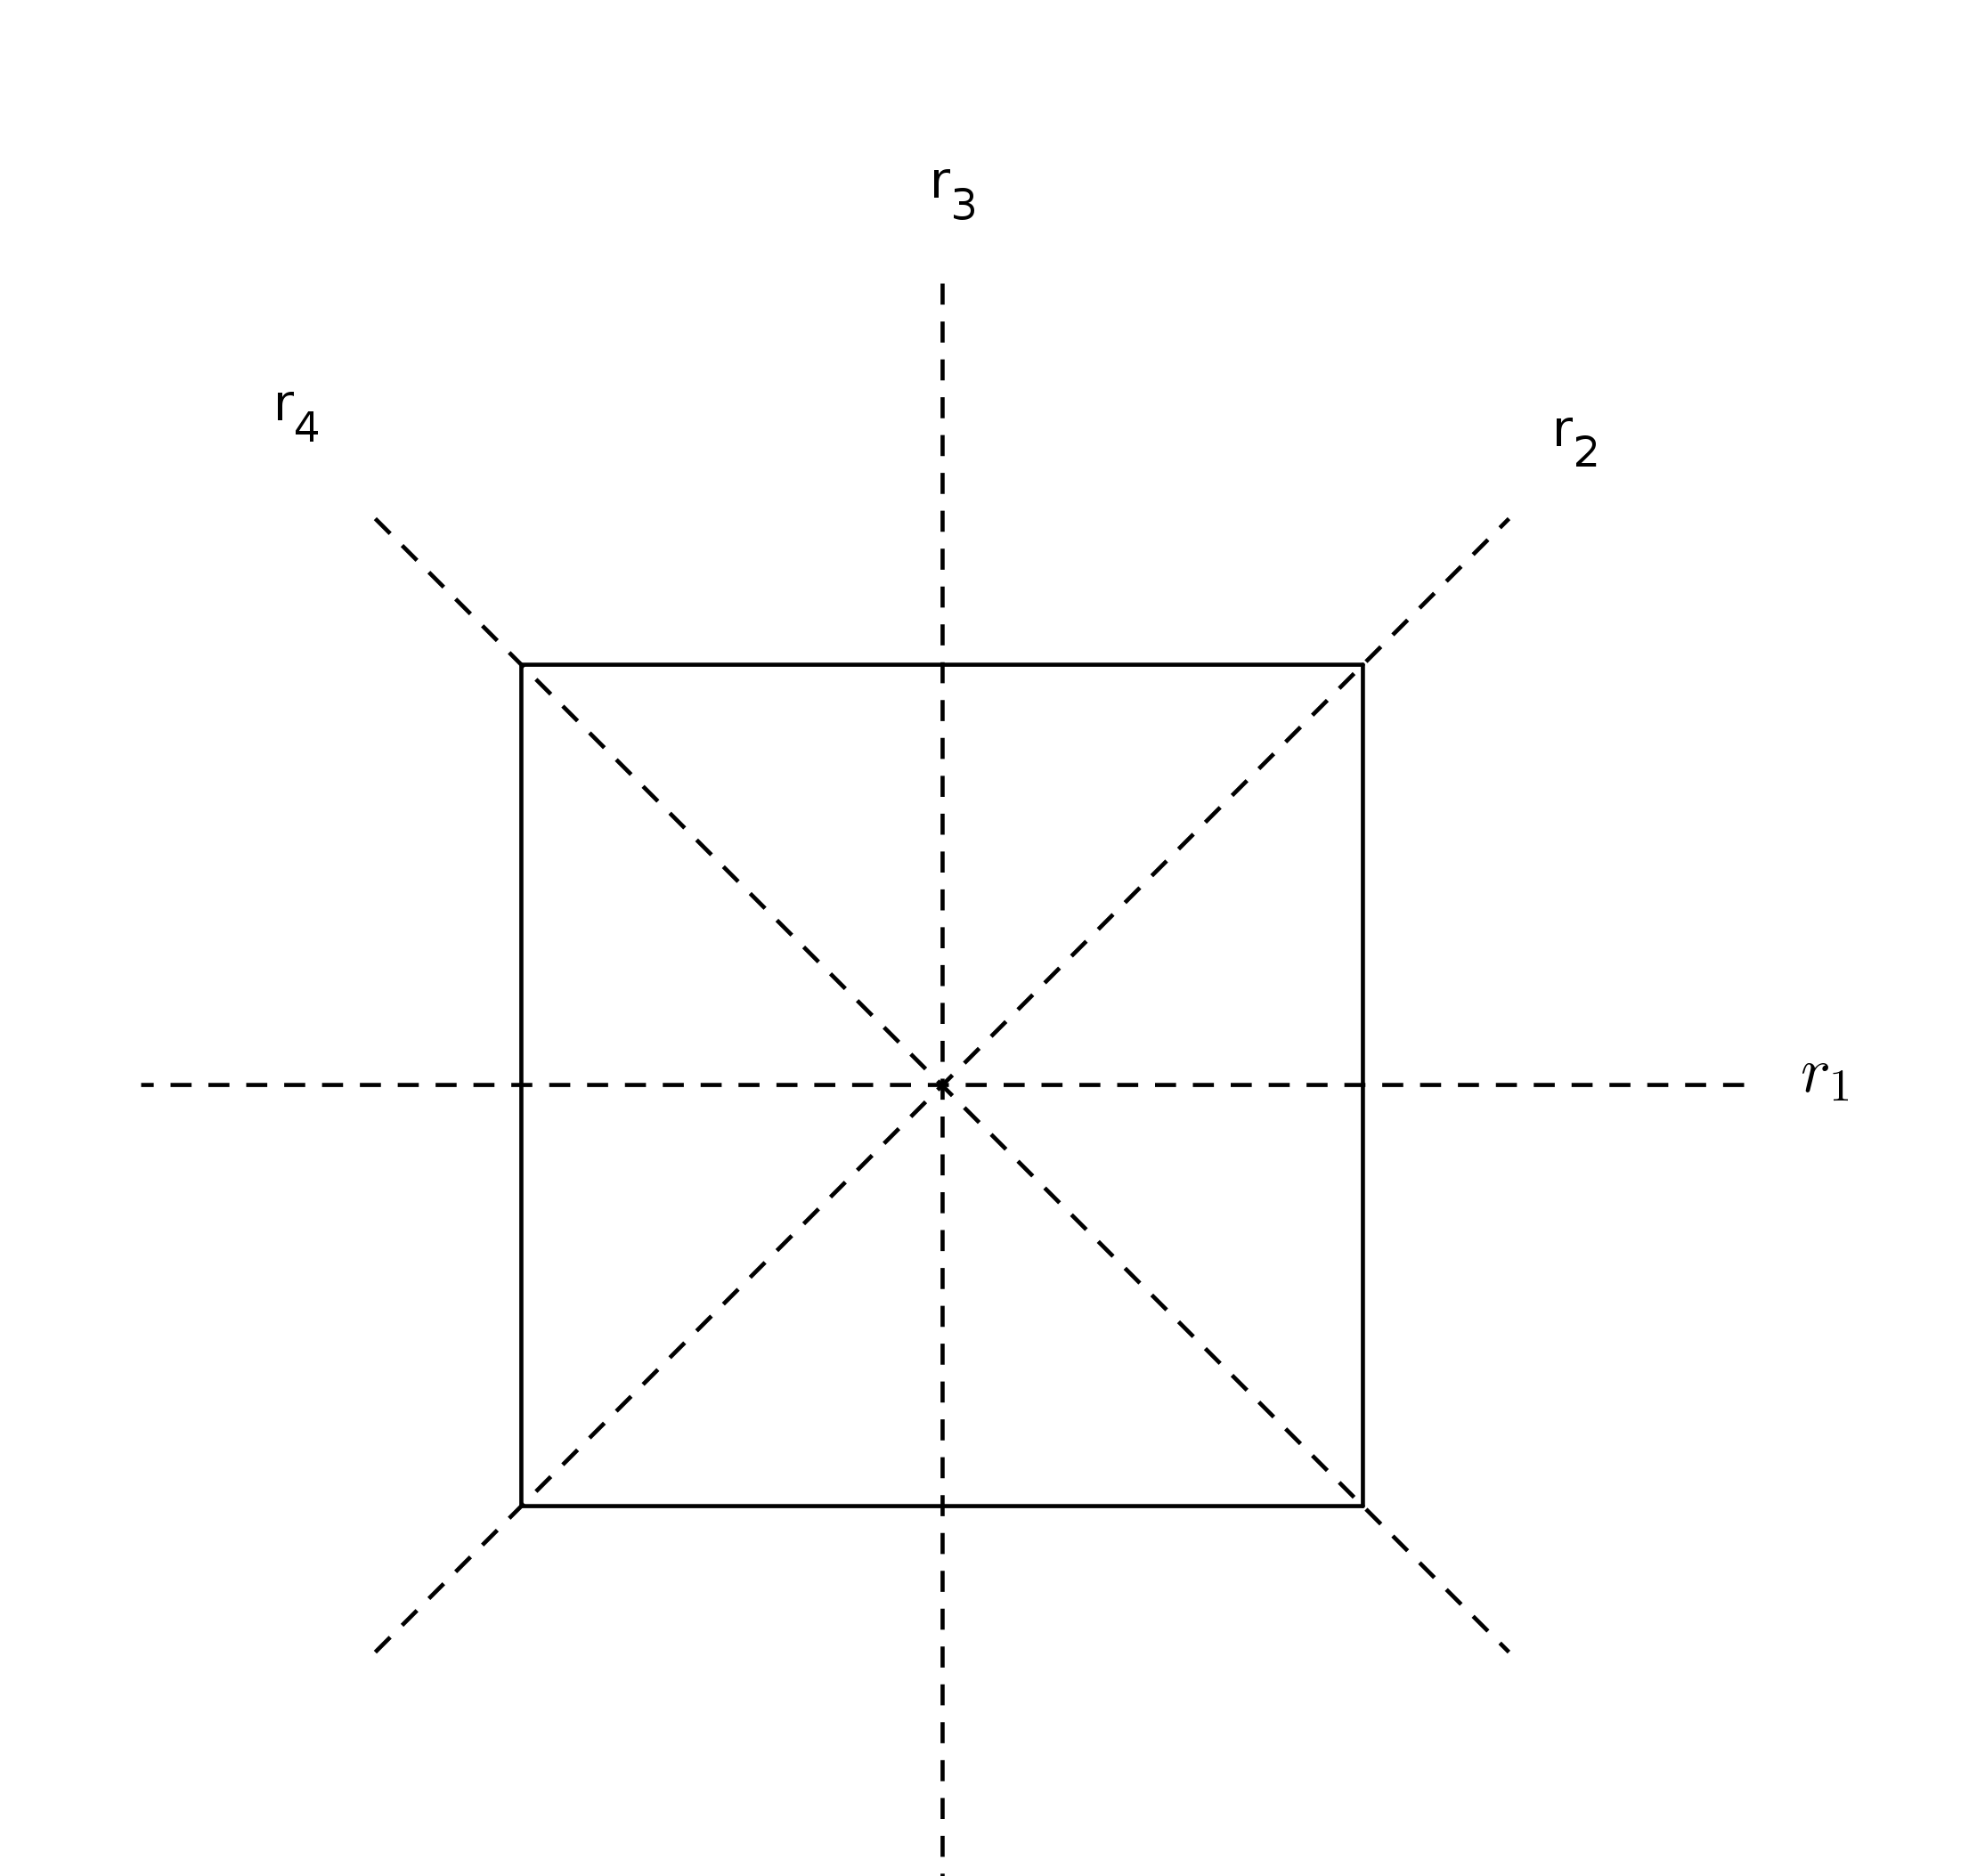
\includegraphics{cuadrado}
	  \captionsetup[figure]{textfont = normal, labelformat=empty, labelsep=period}
	  \vskip 1.80em
  	  \caption*{Fuente: elaboración propia, con programa para computadora geogebra.}
  \label{fig:ejemplo}
\end{figure}
Sea $a$ la rotación de ángulo $\frac{\pi}{2}$ y $b$ la reflexión a través del eje $r_2$. Es fácil ver, bajo consideraciones geométricas, que cualquier otro elemento de este grupo se puede obtener por medio de $a$ y $b$.

De manera más abstracta, este grupo que es llamado grupo diédrico de orden ocho y usualmente denotado por $D_4$, puede ser definido con dos generadores que satisfacen las relaciones:
\begin{equation*}
a^4 = 1, \quad b^2 = 1 , \quad baba = 1.  
\end{equation*}
\indent Por lo tanto este grupo puede ser descrito  como: 
\begin{equation*}
D_4 = \{ 1, a, a^2, a^3, b, ab, a^2b, a^3b \}. 
\end{equation*}
\indent Como todas los elementos de este grupo están en términos de $a$ y $b$, entonces para encontrar una representación matricial $A \colon D_4 \to GL(n,K)$ sobre el campo $K$, será suficiente encontrar matrices $A(a)$, $B(b)$ tales que $A(a)^4 = I$, $A(b)^2 = I$, $A(b)A(a)A(b)A(a) = I.$

Es fácil determinar representaciones de grado uno para $D_4$ en un campo $K$ de característica diferente a dos, de la siguiente manera:
\begin{equation*}
\begin{aligned}
A(a) & = 1\\
B(a) & = 1 \\ 
C(a) & = -1 \\
D(a) & = -1
\end{aligned}
\qquad 
\begin{aligned}
A(b) & = 1\\
B(b) & =  -1 \\
C(b) & = 1 \\
D(b) & = -1.
\end{aligned}
\end{equation*}
\indent Pensando en el significado geométrico de $a$ y $b$, como dos funciones del plano al plano, se puede calcular sus matrices con respecto a la base canónica para obtener otra representación matricial de $D_4$:
\begin{equation*}
\begin{aligned}
W(a) = \begin{pmatrix}
0 & -1 \\
1 & 0
\end{pmatrix}
\end{aligned}
\qquad \text{,} \qquad
\begin{aligned}
W(b) &= \begin{pmatrix}
 0 & 1 \\
 1 & 0
\end{pmatrix}. 
\end{aligned}
\end{equation*}
\end{ejemplo}

\begin{ejemplo}[Suma directa de representaciones]
Sean $T \colon G \to GL(V)$ y $S \colon G \to GL(W)$ dos representaciones de un grupo $G$ sobre un anillo conmutativo $R$. Se puede definir una nueva representación $V \oplus W$, que es llamada la suma directa de dos representaciones dadas y se denota como $T \oplus S$, de la siguiente manera: \begin{equation*} (T \oplus S)_g = T_g \oplus S_g, \quad \mbox{para cada } g \in G. \end{equation*}

Si se eligen bases $\{v_1, \dots, v_n\}$ y $\{ w_1, \dots, w_m \}$ de $V$ y $W$ respectivamente y se denota por $g \mapsto A(g)$ y $g \mapsto B(g)$ las correspondientes representaciones matriciales en las bases dadas, entonces la representación matricial asociada a $T \oplus S$ con respecto a la base $\{ (v_1,0), \dots , (v_n), (0,w_1), \dots, (0,w_n)  \}$ de $V \oplus W$, viene dada por
\begin{equation*} g \mapsto \begin{pmatrix}
A(g) & 0 \\
0 & B(g)
\end{pmatrix}. \end{equation*}
\end{ejemplo}
Los ejemplos anteriormente expuestos, sirven de motivación para introducir algunos conceptos de teoría de la representación. En este trabajo se restringirán las representaciones al caso en el cual $R$ es un campo, debido a que con este caso se logra ilustrar la relación de teoría de representación con los problemas de grupo-anillos.

Primero considérese $T \colon G \to GL(V)$ una representación de un grupo $G$ sobre un campo $K$ y asúmase que $\phi \colon V \to W$ es un isomorfismo de espacios vectoriales sobre $K$. Entonces se puede definir una nueva representación $\overline{T} \colon G \to GL(W)$ por medio de $\overline{T_g} \colon \phi \circ T_g \circ \phi^{-1}$ para todo $g \in G$. Esto es, esencialmente, una copia de $T$. La relación entre estas dos representaciones está ilustrada en el diagrama de la figura \ref{fig:ejemploSumaRepresentaciones}, 
\captionsetup[figure]{labelformat=simple, labelsep=period}
\begin{figure}[t]
  \centering
  \caption{\hskip 2em Diagrama conmutativo para representaciones equivalentes}
  	  \vskip -0.59em 
  	  \[\xymatrix { V \ar[r]^{T_g} 
  	  \ar[d]_{\phi}
  	   & V \ar[d]^{\phi} \\
  	  W \ar[r]_{\overline{T_g}} & W}\]
	  \captionsetup[figure]{labelformat=simple, labelsep=period}
	  \vskip 0.20em
  	  \caption*{Fuente: elaboración propia, con programa para computadora xymatrix.}
  \label{fig:ejemploSumaRepresentaciones}
\end{figure}
lo cual sugiere la siguiente:
\begin{definicion}
Dos representaciones $T \colon G \to GL(V)$ y $\overline{T} \colon G \to GL(W)$ de un grupo $G$ sobre el mismo campo $K$ se dicen que son equivalentes si existe un isomorfismo $\phi \colon V \to W$ tal que $\overline{T_g} = \phi T_g \phi^{-1} $ para cualquier $g \in G$.
\end{definicion}
\begin{definicion}
Dos representaciones matriciales $A \colon G \to GL(n,K)$ y $B \colon G \to GL(n,K)$ de un grupo $G$ sobre un campo $K$ se dicen equivalentes si existe una matriz invertible $U \in GL(n,K)$ tal que $A(g) = UB(g)U^{-1}$ para cualquier $g \in G$.
\end{definicion}

\begin{ejemplo}\label{ejemciclico}
Sea $G$ un grupo cíclico de orden $m$ y $K$ un campo que contiene a $\{ \xi_1, \xi_2, \dots, \xi_m \}$, el conjunto de todas las raíces distintas de la unidad de orden $m$. Entonces, si se consideran las representaciones $B$ y $\Gamma$ dadas en el ejemplo \ref{rciclica} con: 
\begin{equation*} \mathsf{U} = \begin{pmatrix}
\xi_1 & \xi_1^2 & \cdots & \xi_1^m \\
\xi_2 & \xi_2^2 & \cdots & \xi_2^m \\
 & & \cdots & \\
 \xi_m & \xi_m^2 & \cdots & \xi_m^m \\ 
\end{pmatrix}. \end{equation*}
\indent Es claro que $\mathsf{U} \in GL(n,K)$, ya que $\mathsf{U}$ es una matriz de Vandermonde con $det(\mathsf{U}) = \prod_{1 \leq i < j \leq m}(\xi_i - \xi_j) \neq 0$. Entonces, calculando, por un lado se tiene: 
\begin{equation*} B(a)\mathsf{U} = \begin{pmatrix}
\xi_1 & 0 & \cdots & 0\\
0 & \xi_2 & \cdots & 0\\
 & & \cdots & \\
 0 & 0 & \cdots & \xi_m
\end{pmatrix} \begin{pmatrix}
\xi_1 & \xi_1^2 & \cdots & \xi_1^m \\
\xi_2 & \xi_2^2 & \cdots & \xi_2^m \\
 & & \cdots & \\
 \xi_m & \xi_m^2 & \cdots & \xi_m^m
\end{pmatrix} = \begin{pmatrix}
\xi_1^2 & \xi_1^3 & \cdots & \xi_1 \\
\xi_2^2 & \xi_2^3 & \cdots & \xi_2 \\
 & & \cdots & \\
\xi_m^2 & \xi_m^2 & \cdots & \xi_m
\end{pmatrix}, \end{equation*} similarmente: \begin{equation*} 
\mathsf{U}\Gamma(a) = 
\begin{pmatrix}
\xi_1 & \xi_1^2 & \cdots & \xi_1^m \\
\xi_2 & \xi_2^2 & \cdots & \xi_2^m \\
 & & \cdots & \\
 \xi_m & \xi_m^2 & \cdots & \xi_m^m \\
\end{pmatrix}
\begin{pmatrix}
0 & 0 & \cdots & 1 \\
1 & 0 & \cdots & 0 \\
 & & \cdots & \\
0 & 0 & \cdots & 1 \\
\end{pmatrix} = \begin{pmatrix}
\xi_1^2 & \xi_1^3 & \cdots & \xi_1 \\
\xi_2^2 & \xi_2^3 & \cdots & \xi_2 \\
 & & \cdots & \\
\xi_m^2 & \xi_m^2 & \cdots & \xi_m
\end{pmatrix}
\end{equation*} con lo que se ha demostrado que $A(g) = \mathsf{U}B(g)\mathsf{U^{-1}}$, para cualquier $g \in G$ y concluye que $B$ y $\Gamma$ son equivalentes. 
\end{ejemplo}

Considérese $T \colon G \to GL(V)$ una representación de un grupo $G$ sobre el campo $K$, con espacio de representación $V$ y supóngase que $V$ contiene un subespacio $W$ que es invariable bajo $T$, esto es, un subespacio tal que $T_g(W) \subset W$, para cualquier $g \in G$. Entonces se puede considerar el homomorfismo de grupos que asigna a cada elemento $g \in G$ la restricción de $T_g$ al subespacio $W$. Por ser $T_g$ la restricción, es claro que el homomorfismo anterior es una representación de $G$ sobre $K$, con espacio de representación $W$.

Con el afán de dar una representación matricial de este hecho, considérese una base $\{ w_1, w_2, \dots, w_t \}$ de $W$ y extiéndase a una base $ \{ w_1, \cdots, w_t, v_{t+1}, \cdots, v_n \}$ de $V$. Entonces la matriz asociada a cada función $T_g$, $g \in G$ con respecto a esa base es de la forma:
\begin{equation*} \begin{pmatrix}
A(g) & B(g) \\
0 & C(g)
\end{pmatrix} \end{equation*} donde $A(g) \in GL(t,K), C(g) \in GL(n-t,K)$ y $B(g)$ es una matriz de $t \times (n-t)$. Estas consideraciones sugieren la siguiente:
\begin{definicion}
Una representación $T \colon G \to GL(V)$ de un grupo $G$ sobre un campo $K$ es llamada irreducible si los únicos subespacios propios de $V$ que son invariantes bajo $T$ son los triviales, es decir, $V$ y $\{ 0 \}$.
\end{definicion}

La representación es llamada reducible si $V$ contiene  subespacios no triviales que son invariantes bajo $T$. 

\begin{definicion}
Una representación matricial $M \colon G \to GL(n,K)$ es llamada reducible si existe una matriz $\mathsf{U} \in GL(n,K)$ tal que para cualquier $g \in G$, se tiene que la matriz $\mathsf{U}M(g)U^{-1}$ es de la forma
\begin{equation*}
\mathsf{U}M(g)U^{-1} = \begin{pmatrix}
A(g) & B(g) \\
0 & C(g)
\end{pmatrix}. 
\end{equation*}  
\end{definicion}

El ejemplo \ref{ejemciclico} muestra que la representación regular de un grupo cíclico de orden $m$, sobre un campo $K$ que contiene raíces de la unidad de orden $m$, es reducible. De hecho, cualquier representación regular de un grupo finito $G \neq \{ 1 \}$ sobre cualquier campo es reducible. En efecto, nótese que si en el espacio de representación $RG$ se toma el elemento $\hat{G} = \sum_{g \in G}g$ entonces $ T_g(\hat{G}) = \hat{G}$ por lo tanto el subespacio generado por $\hat{G}$ es invariante bajo $T$ y $(\hat{G}) \neq RG.$  

\begin{definicion}
Una representación $T \colon G \to GL(V)$ de un grupo $G$ sobre un campo $K$ es llamada completamente reducible si para todo subespacio $W$ que es invariante bajo $T$ existe un subespacio invariante $W'$ tal que $V = W \oplus W'$.
\end{definicion}
Para entender de mejor manera esta definición, se dará una interpretación en términos de matrices.

Sea $\{ w_1, w_2, \dots, w_t \}$ y $\{ w_{t+1}, \dots, w_n\}$ bases dadas para $W$ y $W'$ \mbox{respectivamente}, entonces $\{ w_1, w_t, w_{t+1}, \dots, w_n \}$ es una base de $V$ y para cualquier $g \in G$ la matriz de $T_g$ con respecto a esta base es de la forma
\begin{equation*} \begin{pmatrix}
A(g) & 0 \\
0 & B(g)
\end{pmatrix} \end{equation*} donde $A(g)$ y $B(g)$ son las matrices de representación de $T_g$ en $W$ y $W'$ con respecto a las bases dadas. 

\begin{definicion}
Una representación matricial $M \colon G \to GL(n,K)$ es llamada completamente reducible si cualquier representación matricial $M$ de la forma 
\begin{equation*} \begin{pmatrix}
A(g) & B(g) \\
0 & C(g)
\end{pmatrix} \end{equation*} es equivalente a una representación matricial de la forma:
\begin{equation*} \begin{pmatrix}
A(g) & 0 \\
0 & D(g) 
\end{pmatrix}. \end{equation*}
\end{definicion}


\section{\hskip 1em Representación y módulos}
 En esta sección se estudiará la conexión que hay entre módulos y \mbox{representaciones}. Dicha conexión se establece usando el concepto de grupo-anillo.
 
 \begin{proposicion}\label{prop:biyeccionModulos}
 Sea $G$ un grupo y $R$ un anillo conmutativo con unidad. Entonces, existe una biyección entre representaciones de $G$ sobre $R$ y $RG\mbox{-módulos}$ libres y de rango finito. 
 \end{proposicion}
 \begin{proof*}
 Dada una representación $T \colon G \to GL(V)$ de $G$ sobre $R$, se asocia a ella el $RG\mbox{-módulo}$ construido a partir de $V$ manteniendo la misma estructura aditiva y definiendo el producto de un elemento $v \in V$ por un escalar $\alpha = \srg{g}{G}{a} \in RG$ como: 
 \begin{equation}\label{defproducto}
 \alpha v = \left( \srg{g}{G}{a}  \right)v = \sum_{g \in G}a(g)T_g(v).
 \end{equation}
 
 Usando está definición de producto se verifica:
 \begin{bulletList}
 \newItem Distributividad de la suma de escalares respecto al producto por escalar \begin{eqnarray*}
  (\alpha + \beta)v &=& \left( \sum_{g \in G}(a_g + b_g)g  \right)v \\
   &=& \sum_{g \in G}(a_g + b_g)T_g(v) \\
   &=& \sum_{g \in G}a_gT_g(v) + \sum_{g \in G}b_gT_g(v) \\
    &=& \alpha v + \beta v .
 \end{eqnarray*}
 \newItem Distributividad de la  suma de elementos del módulo respecto al producto por escalar
 \begin{eqnarray*}
 \alpha(v + w) &=& \left(\srg{g}{G}{a}(v + w)  \right) \\
  &=& \sum_{g \in G}a_gT_g(v+w) \\
  &=& \sum_{g \in G}a_gT_g(v) + \sum_{g \in G}a_gT_g(w) \\
  &=& \alpha v + \alpha w .
 \end{eqnarray*}
 \newItem Para la asociatividad, por un lado se tiene
 \begin{eqnarray*}
 \alpha(\beta v) &=& \left( \sum_{h \in G}a(g)h \right)\left( \sum_{g \in G}b(g)T_g(v) \right) \\
  &=& \sum_{h \in G}a(h)T_h\left( \sum_{g \in G}b(g)T_g(v)  \right) \\
  &=& \sum_{h, g \in G}a(h)b(g)T_{hg}(v).
 \end{eqnarray*}
 
 Por otro lado se tiene:
 \begin{eqnarray*}
 (\alpha\beta)v &=& \left( \sum_{h,g \in G}a(h)b(g)hg  \right)(v)\\
  &=& \sum_{h,g \in G}a(h)b(g)T_{hg}(v)
 \end{eqnarray*}
 con lo que se comprueba que $\alpha(\beta v) = (\alpha\beta)v$.
 \newItem Considérese $\alpha = 1_{G}$, entonces
 \begin{eqnarray*}
 \alpha v &=& T_{1_G}(v)\\
  &=& I(v) \\
  &=& v.
 \end{eqnarray*}
 \end{bulletList}
  \hskip 1cm Por lo expuesto anteriormente es fácil notar que la multiplicación por escalar definida en la ecuación~\eqref{defproducto} induce un $RG\mbox{-módulo}$.
 
 Al converso, si $M$ es un $RG\mbox{-módulo}$ de rango finito sobre $R$, se define la representación de $G$ sobre $R$ asignando a cada elemento $g \in G$ el $R\mbox{-automorfismo}$ $T_g \colon M \to M$ dado por $T_g(m) = gm$.
 
 Nótese que dado $T \colon G \to GL(V)$ una representación de $G$ sobre $R$ y $M$ su $RG\mbox{-módulo}$ inducido, se tiene que $S$, la representación inducida por $M$, es tal que $S_g(m) = gm = \alpha m \simeq T_g(m)$, donde $\alpha$ es la imagen de la inmersión de $G$ en $RG$ dada en el teorema~\ref{inmersion}.
 
 De manera similar, dado $M$ un $RG\mbox{-módulo}$ y $S \colon G \to GL(M)$ su representación inducida, entonces su $RG\mbox{-módulo}$ inducido por la ecuación~\eqref{defproducto} deja invariante a $M$. Por lo tanto se ha demostrado que las aplicaciones construidas anteriormente son inversas la una de la otra. 
 \end{proof*}
  Como ejemplo, considérese  un grupo finito $G$ y $RG$ como un módulo sobre sí mismo, de esta forma $RG$ es de rango finito $|G|$ sobre $R$. Entonces, dado un elemento $x \in G$, la representación $T_x \colon RG \to RG$ viene dada por: \begin{equation*}T_{x}\left( \sum_{g \in G}a(g)g\right) = x\left( \sum_{g \in G}a(g)g\right) = \left( \sum_{g \in G}a(g)gxg\right).\end{equation*}
  
  Esto significa que $x \in G$ actúa en los elementos de la base $G = \{ g_1, \dots, g_n \}$ multiplicándolos por la izquierda. En otras palabras, la representación asociada al $RG\mbox{-módulo}$ $RG$ es precisamente la representación regular de $G$. 
\begin{lema}
  Sea $T \colon G \to GL(V)$ una representación de un grupo $G$ sobre un campo $K$, con espacio de representación $V$, entonces un subespacio $W \subset V$ es invariante bajo $T$ si y solo si $W$ es un $KG\mbox{-módulo}$ de $V$. 
  \end{lema}
  \begin{proof*}
  Se procede a demostrar este hecho en dos partes:
  \begin{bulletList}
  \newItem Sea $W \subset V$ invariante bajo $T$, entonces $T_{g}(W) = W$ para cualquier $g \in G$. Sean $w_1, w_2 \in W$ se tiene que $T_{g}(w_1 + w_2) = T_{g}(w_1) + T_{g}(w_2) \in W$, así $T_{g}^{-1}(T_{g}(w_1 + w_2)) \in W$. Por otra parte, si se considera $\alpha = \sum_{g \in G}a(g)g$ entonces $\alpha w = \sum_{g \in G}a(g)T_g(w) \in W$ y por lo tanto $W$ es un $KG\mbox{-módulo}$ de~$V$.
  \newItem Sea $W$ subespacio de $V$, $W \subset V$ y $W$ un $KG\mbox{-módulo}$ de $V$, entonces para $w \in W$ y $g \in RG$ se tiene $gw = 1\cdot T_g(w) \in W$. \qedhere
  \end{bulletList} 
  \end{proof*}
  
  \begin{teorema}\label{teo:relacionTG}
  Sea $G$ un grupo y $K$ un campo. Entonces:
  \begin{bulletList}
  \newItem Dos representaciones $T$ y $T'$ de $G$ sobre $R$ son equivalentes si y solo si los correspondientes $RG\mbox{-módulos}$ son isomorfos.
  \newItem Una representación es irreducible (o completamente reducible) si y solo si el correspondiente $RG\mbox{-módulo}$ es irreducible (o completamente reducible).
  \end{bulletList}
  \end{teorema}
  \begin{proof*}
  Se procede a demostrar este lema por incisos:
  \begin{bulletList}
  \newItem Supóngase que $T$ y $T'$ son representaciones de $G$ sobre $K$ equivalentes, entonces existe $\phi \colon V \to W$ isomorfismo, donde $V$ y $W$ son los espacios de representación de $T$ y $T'$ respectivamente, tal que $T'_g = \phi T_g \phi^{-1}$ para cualquier $g \in G$. Entonces se probará que $\phi$ es isomorfismo de $RG\mbox{-módulos}$ también.  En efecto
  \begin{eqnarray*}
   \phi(\alpha v) &=& \phi\left( \sum_{g \in G}a(g)T_g(v) \right) \\ 
   &=&  \sum_{g \in G}a(g)\phi(T_g(v)) \\
    & =& \sum_{g \in G}a(g)T'_g(\phi(v))\\ 
    &=& \alpha \phi(v).
  \end{eqnarray*}
   \newItem Supóngase que $M$ y $N$ son $RG\mbox{-módulos}$ isomorfos, entonces existe $f \colon M \to N$ isomorfismo de $RG\mbox{-módulos}$. Sean $T$ y $T'$ las representaciones inducidas por $M$ y $N$ respectivamente, entonces:
   \begin{eqnarray*}
   (fT_gf^{-1})(n) &=& 
    f\left(T_g\left(f^{-1}(n)\right)\right)\\
    &=& f\left(gf^{-1}(n)\right) \\
    &=& gf\left(f^{-1}(n)\right) \\
    &=& gn \\
    &=& T'_g(n)
   \end{eqnarray*} con lo que se comprueba que $T$ y $T'$ son equivalentes. 
   
   \newItem Si una representación $T$ es irreducible, entonces los únicos subespacios de $V$ que son invariantes bajo $T$ son los triviales y, por el lema anterior, los únicos submódulos de $M$, el módulo inducido por $T$, son los los triviales. De manera análoga se puede demostrar el converso. \qedhere
   \end{bulletList}
  \end{proof*}
  También es posible notar que si un $RG\mbox{-módulo}$ $M$ admite una descomposición como suma directa de submódulos $M = \oplus_{i = 1}^{t}M_i$ y si $T$ y $T_i$ denota las representaciones correspondientes a estos módulos, entonces $T = \oplus_{i = 1}^tT_i$. 
 
 En lo que sigue, se mostrará como la información que ya se conoce acerca de los grupo-anillos, se puede trasladar a términos de representaciones de grupos. 
 
 El lector deberá recordar que en el corolario \ref{cor:car}, como consecuencia directa del teorema de Maschke, se demostró que si $K$ es un campo tal que $\car(K) \nmid |G|$, entonces $KG$ es un anillo semisimple. Además, se demostró en el teorema \ref{teo:wa} que en este caso todo $KG\mbox{-módulo}$ es simple. Por lo tanto, en particular, se sigue inmediatamente que todo $KG\mbox{-módulo}$ finito dimensional sobre $K$ se puede escribir como suma directa de módulos irreducibles.
 
 En términos de representaciones, esto significa que bajo estas condiciones, toda representación de $G$ sobre $K$ es la suma directa de representaciones irreducibles. Así, para determinar todas las representaciones de $G$ sobre $K$, mediante equivalencia, es suficiente determinar todos los $KG\mbox{-módulos}$ irreducibles, salvo isomorfismos. 
 
 Ahora, es necesario hacer uso del teorema de Wedderburn-Artin, aplicado a grupo-anillos (teorema \ref{teo:wa}), el cual establece que el número de $KG\mbox{-módulos}$ irreducibles que no son isomorfos entre sí, es precisamente el número de componentes simples de $KG$ y estas están determinadas exclusivamente por la estructura de $KG$.
 
 En particular, es importante recordar que si se escribe $KG$ en la forma:
 \begin{equation*} KG \simeq \oplus_{i = 1}^{r}M_{n_i}(D_i) \end{equation*} donde $D_i, 1\leq i \leq r$, son anillos de división que contienen a $K$ en sus centros, y si se calcula la dimensión en ambos lados de la ecuación, se tiene
 \begin{equation*} |G| = \sum_{i = 1}^{r}n_{i}^2[D_i:K]. \end{equation*}
 
 Por otro lado, se sabe que el módulo irreducible $I_i$ correspondiente a la componente simple $M_{n_i}(D_i)$ es isomorfo a $D_{i}^{n_i}$. Como el grado de la correspondiente representación $T_i$ viene dado por la dimensión de este módulo sobre $K$, se obtiene que
 \begin{equation*}  \grado (T_i) = [D_{i}^{n_i}:K] = n_i[D_i:K] \end{equation*} así, se puede escribir: \begin{equation*} |G| = \sum_{i = 1}^{r}n_i\grado(T_i). \end{equation*} 
 
 \begin{ejemplo}
 Se mostró  en el ejemplo \ref{ejem:orden7} que si $G = \langle a \rangle$ denota al grupo cíclico de orden siete, entonces:
 \begin{equation*} \mathds{Q}G \simeq \mathds{Q}\oplus\mathds{Q}(\zeta), \end{equation*} donde $\zeta$ denota una raíz primitiva de la unidad de orden siete. De lo anterior, las componentes simples de $\mathds{Q}G$ son anillos de matrices de $1\times 1$ sobre los anillos $\mathds{Q}$ y $\mathds{Q}(\zeta)$ respectivamente y por ende existen solamente dos representaciones irreducibles que no son equivalentes, $S$ y $T$ de $G$ sobre $\mathds{Q}$, con grados
 \begin{equation*} \grado(S) = [\mathds{Q}:\mathds{Q}] = 1, \quad \grado(T) = [\mathds{Q}:\mathds{Q}] = 6. \end{equation*} 
 
 Como las representaciones $1\mbox{-dimensionales}$ son equivalentes si y solo si son iguales y como cualquier grupo admite la representación trivial $S \colon G \to GL(1,\mathds{Q})$ dada por $S_g = 1$, para cada $g \in G$, entonces la representación $1\mbox{-dimensional}$ de $G$ sobre $\mathds{Q}$ es la trivial.
 
 Para determinar $T_a$, de acuerdo a las consideraciones anteriores, se debe considerar el $\mathds{Q}G\mbox{-módulo}$ irreducible $I_2 = D_2^{n_2}$ correspondiente a la segunda componente simple de $\mathds{Q}$. Entonces, la representación $T \colon G \to GL(I_2)$ está dada por $T_a(v) = av$, para cada $v \in I_2$. En este caso, $n_2 = 1$ y $D_2 = \mathds{Q}(\zeta)$, así que $I_2 = \mathds{Q}(\zeta)$, donde la multiplicación por un elemento $\alpha = (\alpha_1, \alpha_2) \in \mathds{Q}G$ está dada por $\alpha v = \alpha_2v$, para todo $v \in \mathds{Q}(\zeta)$. Recordando que el elemento $a \in \mathds{Q}(\zeta)$ le corresponde, vía isomorfismo, el elemento $(1,\zeta) \in \mathds{Q}\oplus\mathds{Q}(\zeta)$ se tiene
 \begin{equation*} T_a(v) = av = \zeta v, \quad v 
 \in \mathds{Q}(\zeta). \end{equation*} Por lo tanto, si se toma $\{ 1, \zeta, \zeta^2, \dots, \zeta^5 \}$ como una base de $\mathds{Q}(\zeta)$ sobre $\mathds{Q}$, entonces la correspondiente matriz está dada por
 \begin{equation*} A(a) = \begin{pmatrix}
 0 & 0 & 0 & 0 & 0 & -1 \\
 1 & 0 & 0 & 0 & 0 & -1 \\
 0 & 1 & 0 & 0 & 0 & -1 \\
 0 & 0 & 1 & 0 & 0 & -1 \\
 0 & 0 & 0 & 1 & 0 & -1 \\
 0 & 0 & 0 & 0 & 1 & -1
 \end{pmatrix}. \end{equation*}
 \end{ejemplo}
 \begin{ejemplo}[Representaciones del grupo diédrico de orden ocho.]
 Se ha probado en ele ejemplo \ref{ejem:diedrico} que el grupo $D_4$ admite cuatro representaciones distintas de grado uno y una representación $W$ de grado dos sobre $\mathds{Q}$, por lo tanto existen cuatro componentes simples isomorfas a $\mathds{Q}$. Sean $M_n(D)$ la componente simple correspondiente a la representación de grado dos. Como $2 = \grado(W) = n[D:\mathds{Q}]$, entonces $n = 1$ y $[D:\mathds{Q}]$ o $n = 2$ y $[D:\mathds{Q}] = 1$.
 
 Para el primer caso, se puede observar que $\mathds{Q}D_4$ debe ser de la forma \begin{equation*} \mathds{Q}D_4 \simeq \mathds{Q} \oplus \mathds{Q} \oplus \mathds{Q}\oplus\mathds{Q}\oplus D\oplus D',\end{equation*} donde $D'$ es una anillo de división con $[D':\mathds{Q}] = 2$. Es fácil notar que un anillo de división de dimensión dos sobre un campo tiene que ser conmutativo, entonces $\mathds{Q}D_4$ es conmutativo, lo cual es una contradicción, ya que $D_4$ no es abeliano. 
 
 En consecuencia, se debe tener que $n = 2$ y $D = \mathds{Q}$. De esta forma \begin{equation*}  \mathds{Q}D_4 \simeq \mathds{Q}\oplus\mathds{Q}\oplus\mathds{Q}\oplus\mathds{Q}\oplus M_{2}(\mathds{Q}). \end{equation*}
 \end{ejemplo}
 


\addtocontents{toc}{\protect\addvspace{1.8em}}
\chapter{ELEMENTOS ALGEBRAICOS}

\section{\quad Generalidades y definiciones}
En este capítulo será de especial interés estudiar algunos elementos algebraicos en grupo-álgebras usando la representación regular que puede ser definida para un álgebra finito dimensional con unidad sobre un campo $K$ de la siguiente manera.

\begin{definicion}
Sea $T \colon A \to \hom_K(A,A)$ tal que $a \mapsto T_a \in \hom_K(A,A)$, definida mediante multiplicación por la izquierda por $a$. Esto es, $T_a$ es una aplicación tal que $T_a(x) = ax$, para cualquier $x \in A$.  
\end{definicion}

Se puede observar a partir de la definición que
\begin{eqnarray*}
T_{a+b} &=& T_a + T_b \\
T_{ab} &=& T_aT_b \\
T_{ka} &=& kT_a
\end{eqnarray*}
para todo $a,b \in A,$  $k\in K$. Mas aún, la aplicación $a \mapsto T_a$ es inyectiva debido a que $T_a(1) = a$. Eligiendo una base $\{ a_1, \dots, a_n \}$ de $A$ sobre $K$ se puede representar a $T_a$ con una matriz $\rho(a)$, con lo que  se obtiene la representación matricial:
\begin{equation*}
a \mapsto \rho(a) \in M_n(K).
\end{equation*}
Si $a$ es un elemento algebraico de $A$, esto es, si existe un polinomio no nulo $f(X) \in K[X]$ tal que $f(a) = 0$, entonces los valores propios de la matriz $\rho(a)$ también anulan a $f(X)$, debido al teorema de Cayley-Hamilton (véase \cite[241]{bib:lang}). 

De esta manera, por ejemplo, si $a$ es un elemento nilpotente entonces los valores propios de $\rho(a)$ son todos cero. Si $a$ es de orden multiplicativo finito, es decir, si $a^m = 1$ para algún $m$ entero positivo, entonces los valores propios de $\rho(a)$ son raíces de la unidad de orden $m$. 
\begin{lema}\label{lem:traza}
Sea $G$ un grupo finito y $K$ un campo. Sea $p$ la representación regular de $KG$ y $\gamma = \sum_{g \in G}\gamma(g)g \in KG$. Entonces la traza de $\rho(\gamma)$ viene dada por
\begin{equation*}
\tr\rho(\gamma) = |G|\gamma(1).
\end{equation*}
\end{lema} 
\begin{proof*}
Se sabe que $\tr\rho(\gamma)$ es independiente de la base elegida, así que se elige $G=\{g_1, \dots, g_n \}$ como $K$-base para $KG$ y se asume que $g_1=1$.
Entonces
\begin{equation*}
\rho(\gamma) = \rho\left( \sum_{g \in G}\gamma(g)g \right) = \sum_{g \in G}\gamma(g)\rho(g) .
\end{equation*}
Para un elemento $ 1 \neq g  \in G$, se tiene $gg_i \neq g_i$, para $1\leq i\leq n$, de donde se sigue que los elementos de la diagonal de la matriz $\rho(g)$ son todos nulos si $g \neq 1$. Así $\tr\rho(g) = 0$ si $g \neq 1$. Más aún, como $\rho(1)$ es la matriz identidad, se tiene que $\tr\rho(1) = n$. Entonces
\begin{equation*}
\tr\rho(\gamma) = \sum_{g \in G}\gamma(g)\tr(g) = \gamma(1)\tr\rho(1) = \gamma(1)|G|.\qedhere
\end{equation*} 
\end{proof*}

\begin{lema}\label{lem:BH}
Sea $\gamma = \sum_{g \in G}\gamma(g)g$ una unidad de orden finito en el grupo-anillo entero  $\mathds{Z}G$ con $G$ un grupo finito y asúmase que $\gamma(1)\neq 0$. Entonces $\gamma = \gamma(1) = \pm 1.$
\end{lema}
\begin{proof*}
Sea $|G| = n$ y supóngase que $\gamma^{m} = 1$ para algún entero positivo $m$. Si se considera la representación regular $\rho$ del grupo-álgebra $\mathds{C}G$ y a $\mathds{Z}G$ como un subanillo de la misma, se tiene que $\tr\rho(\gamma) = n\gamma(1)$.
Como $\gamma^{m} = 1$, entonces $\left( \rho(\gamma) \right)^m = \rho(\gamma^{m}) = I$, de esto se sigue que $\rho(\gamma)$ es raíz del polinomio $X^m-1$, cuyas raíces son todas distintas. Esto implica, por el teorema espectral (véase \cite[214]{bib:lang}), que existe una base de $\mathds{C}G$ donde la matriz de $\rho(\gamma)$ es diagonal de la forma
\begin{equation*}
\mathds{A} = \begin{pmatrix}
\xi_1 & & & &\\
 & \xi_2 & & \\
 & & \ddots & \\
  & & & \xi_n
\end{pmatrix}, \quad \xi_i^m = 1.
\end{equation*}
 Entonces $\tr\rho(\gamma) = \sum\limits_{i = 1}^{n}\xi_i$ y así
 \begin{equation*}
 n\gamma(1) = \sum\limits_{i =1}^{n}\xi_i.
 \end{equation*}
 
 Por lo tanto, aplicando valor absoluto,
 \begin{equation*}
  |n\gamma(1)| = \left| \sum_{i = 1}^{n}\xi_i \right| \leq \sum_{i = 1}^{n}|\xi| = n.
 \end{equation*}
 Como $|n\gamma(1)| = n|\gamma(1)| \leq n$, entonces $|\gamma(1)| = 1$ y $\left| \sum_{i = 1}^{n}\xi_i \right| = \sum\limits_{i = 1}^{n}| \xi_i|$, lo cual sucede si y sólo si $\xi_1=\xi_2=\cdots = \xi_n$.
 
 Así $n\gamma(1) = n\xi_1$ y $\gamma(1) = \xi_1=\pm 1$. Se concluye que $\rho(\gamma) = \pm I$, de donde, $\gamma = \pm 1$.
\end{proof*}
\begin{corolario}
Supóngase que $\gamma = \sum_{g \in G}\gamma(g)g$ es una unidad central en el grupo-anillo entero $\mathds{Z}G$ con $G$ un grupo finito de orden finito. Entonces $\gamma$ es de la forma $\gamma = \pm g$ con $g \in  \mathcal{Z}(G)$.
\end{corolario}
\begin{proof*}
Sea $\gamma = \sum_{g \in G}\gamma(g)g$ una unidad central de orden $m$. Supóngase que $\gamma(g_0) \neq 0$, para algún $g_0 \in G$. Entonces $\gamma g_0^{-1}$ es también una unidad de orden finito en $\mathds{Z}G$. Mas aún, el coeficiente de $1$ en la expresión de $\gamma g_0^{-1}$ es $\gamma(g_0) \neq 0$, de donde $\gamma g_0^{-1} = \pm 1$ y por lo tanto $\gamma = \pm g_0$.
\end{proof*}
Una consecuencia inmediata del corolario anterior es el siguiente
\begin{teorema}\label{teo:Graham-Higman}
Sea $A$ un grupo abeliano finito. Entonces, el grupo de torsión de las unidades del grupo-anillo entero $\mathds{Z}A$ es igual $\pm A$.
\end{teorema}

Ahora se desea hacer un estudio de los elementos idempotentes. Es evidente que en cualquier anillo con unidad el $0$ y el $1$ son elementos idempotentes, estos elementos son llamados \textbf{idempotentes triviales} de un anillo. Se verá a continuación que los elementos idempotentes $e$ en un grupo-álgebra están fuertemente influenciados por su primer coeficiente $e(1)$.

\begin{teorema}\label{teo:idme}
Sea $G$ un grupo finito y $K$ un campo de característica cero. Supóngase que $e \in KG$ y $e$ es idempotente. Entonces:
\begin{bulletList}
\newItem $e(1) \in \mathds{Q}$.
\newItem $0 \leq e(1) \leq 1$.
\newItem $e(1) = 0 \Leftrightarrow e = 0$ y $e(1) = 1 \Leftrightarrow e=1$.   
\end{bulletList} 
\end{teorema}
\begin{proof*}
Considérese la representación regular de $KG$ escrita con respecto a la base $G$ de $KG$. Entonces, por el lema \ref{lem:traza}, se tiene que $\tr\rho = |G| e(1)$. Más aún, como $e^2 = e$, $\rho(e)$ satisface el polinomio $X^2 - X = X(X-1)$ y por lo tanto $\rho(e)$ puede ser diagonalizada. Los valores propios de $\rho(e)$ son $0$ o $1$ ya que $\rho(e)$ es idempotente. Debido a que la traza es la suma de los donde valores propios, se tiene \ que  $\tr\rho(e) = r$,  donde  $r$  es el número de valores propios iguales a $1$ y por lo tanto también es el  rango de $\rho(e)$. Por lo expuesto anteriormente se puede afirmar que $0\leq e(1) \leq 1$.

Nótese que $e(1) = 0 $ si y sólo si el rango de $\rho(e)$ es $0$ y eso pasa sólo si $e = 0$. Similarmente $e(1) = 1$ si y sólo si el rango de $\rho(e)$ es $\mid G \mid $, lo cual pasa sólo si $\rho(e)$ es la matriz identidad, es decir, si $e = 1$. 
\end{proof*} 
\section{\hskip 1em  Elementos Idempotentes}
Se ha demostrado en el teorema \ref{teo:idme} que si $K$ es un campo de característica cero y $G$ es un grupo finito, entonces cualquier elemento idempotente $e \in KG$ cumple que $e(1) \in \mathds{Q}$. Se dará, en esta sección, un resultado análogo a este resultado, donde $K$ tiene característica $p > 0$.

\begin{teorema}\label{teo:genidem}
Sea $K$ un campo de característica $p > 0$ y sea $G$ cualquier grupo. Supóngase que $e \in KG$ es un idempotente. Entonces $e(1) \in F_p$, donde $F_p$ es el subcampo primo de $K$. 
\end{teorema}

La demostración de este resultado está fuera del alcance de este trabajo, pero se recomienda al lector consultar \cite{bib:passman}. 

En el teorema \ref{teo:idme} se demostró el teorema anterior cuando la característica del campo es cero con la condición de que el grupo sea finito, pero dicho resultado es válido aún cuando el grupo es infinito, pero su demostración requiere el uso de resultados previos de teoría de números. Para la demostración del siguiente resultado, se sugiere al lector consultar \cite{bib:passman}.

\begin{teorema}\label{teo:genidem23}
Sea $G$ un grupo cualquiera y $K$ un campo de característica cero. Supóngase que $e = e^2 = \sum e(g)g \in KG$. Entonces:
\begin{bulletList}
\newItem $e(1) \in \mathds{Q}$.
\newItem $0\leq e(1) \leq 1$.
\newItem $e(1) = 0 \Leftrightarrow e= 0 $ y $e(1) = 1 \Leftrightarrow e = 1$. 
\end{bulletList}
\end{teorema} 

Supóngase que $e = e^2 \in \mathds{Z}G$, como $e(1)$ es un entero, se sigue del teorema anterior que $e = 0$ o $e = 1$. Así, se obtiene el siguiente
\begin{corolario}
El grupo-anillo entero $\mathds{Z}G$ sólo contiene idempotentes triviales, para cualquier grupo $G$.
\end{corolario}
\section{\hskip 1em Unidades de Torsión}
Se demostró en el lema \ref{lem:BH} que si $G$ es un grupo finito, $\gamma \in \mathds{Z}G$ es una unidad de orden finito y $\gamma(1) \neq 0$ entonces $\gamma = \pm 1$. Dicho resultado es válido también cuando $G$ es un grupo infinito. 
\begin{teorema}\label{teo:Passman-Bass}
Sea $\gamma = \sum\gamma(g)g \in \mathds{Z}G$ que satisface $\gamma^n = 1$, para algún entero positivo $n$. Si $\gamma(1) \neq 0$ entonces $\gamma = \pm 1$.
\end{teorema} 
\begin{proof*}
Sea $\mathds{C}[X]$ el anillo de polinomios con coeficientes en $\mathds{C}$. Considérese el homomorfismo $\phi \colon \mathds{C}[X] \to \mathds{C}[\gamma]$ dada por $X \mapsto \gamma$. El kernel de este homomorfismo es el ideal $\langle f(X) \rangle$ generado por el polinomio minimal $f(X)$ de $\gamma$. Entonces $f(X)$ divide a $X^n - 1$ y por lo tanto tiene sus raíces distintas. 
Así, se tiene 
\begin{equation*}
\mathds{C}[\gamma] \simeq \frac{\mathds{C}[X]}{\langle (X) \rangle} \simeq \mathds{C}\oplus\mathds{C}\oplus\cdots\oplus\mathds{C} \simeq \oplus_i\mathds{C}e_i,
\end{equation*}
donde los $e_i$ son idempotentes ortogonales primitivos de $\mathds{C}[\gamma]$. De lo anterior, se puede escribir $\gamma = \sum_{i}\xi_ie_i$ donde $\xi_i\in \mathds{C}$, $\xi_i^n = 1$ y $e_ie_j = \delta_{ij}e_j$, con $\delta_{ij}$ la función delta de Kronecker. 

Calculando el primer coeficiente en ambos lados de la ecuación y usando el teorema \ref{teo:genidem23} se obtiene
\begin{equation*}
\gamma(1) = \sum\xi_ie_i(1) = \sum\xi_i\frac{r_i}{s}, \quad \mbox{con } r_i, s \in \mathds{Z}, \quad r_i,s \geq 0.
\end{equation*}
Entonces, $s\gamma(1) = \sum\xi_ir_i$. De igual manera; como $\sum e_i = 1$ se tiene que $1 = \sum \frac{r_i}{s}$, así $\sum r_i = s$. De donde
\begin{equation*}
|s\gamma(1)| = \left| \sum\xi_ir_i  \right| \leq \sum |\xi||r_i| = \sum |r_i|=s.
\end{equation*}
Como $|s\gamma(1)|\leq s$, se tiene $|\gamma(1)|= 1$ y también $\left| \sum \xi_ir_i \right| = \sum|\xi_i||r_i|$. Se sigue que todos los $\xi_i$ son iguales y $\gamma = \sum \xi_1e_1 = \xi_1 = \gamma(1) \in \mathds{Z}$. 
\end{proof*}

Este último resultado tiene bastantes consecuencias útiles. El lector deberá recordar que, como se mostró en la proposición \ref{prep:conjugacion}, hay una involución estándar en $\mathds{Z}G$ dada por 
\begin{equation*}
\gamma = \sum\gamma(g)g \mapsto \gamma* = \sum\gamma(g)g^{-1},
\end{equation*}
tal que
\begin{eqnarray*}
(\gamma^*)^* &=& \gamma \\
(\gamma + \mu)^* &=& \gamma^* + \mu^*\\
(\gamma\mu)^* &=& \mu^*\gamma^*\\
(c\gamma)^* &=& c\gamma^*,
\end{eqnarray*}
para todo $\gamma, \mu \in \mathds{Z}G$ y $c \in \mathds{Z}$. Más aún, 
\begin{equation*}
(\gamma\gamma^*)(1) = \sum(\gamma(g))^2
\end{equation*}
lo cual implica que $\gamma\gamma^* = 0 $ si y sólo si $\gamma = 0$.

\begin{corolario}
Supóngase que $\gamma \in \mathds{Z}G$ tiene la propiedad de conmutar con $\gamma^*$. Si $\gamma$ es una unidad central de orden finito, entonces $\gamma = \pm g_0$ para algún $g_0 \in G$.
\end{corolario}
\begin{proof*}
Por hipótesis $\gamma^n = 1$ para algún entero positivo $n$ y $\gamma\gamma^* = \gamma^*\gamma$, por lo tanto $(\gamma\gamma^*) = 1$. Más aún, $(\gamma\gamma^*)(1) = \sum \gamma(g)^2 \neq 0$. Entonces, por el teorema anterior, $\gamma\gamma^* = 1$. De esta manera, existe un único coeficiente $\gamma(g_0)$ que es distinto de cero. Se concluye entonces que $\gamma = \pm g_0$. 
\end{proof*}
\begin{corolario}
Todas las unidades centrales de orden finito en $\mathds{Z}G$ son triviales.
\end{corolario}
\begin{corolario}
Si $A$ es un grupo abeliano cualquiera, entonces todas las unidades de torsión de $\mathds{Z}A$ son triviales.
\end{corolario}
\section{\hskip 1em Elementos nilpotentes}
Ahora se desea clasificar los grupo-álgebras $KG$ de un grupo finito $G$ sobre un anillo $K$ tal que $KG$ no tiene elementos nilpotentes no triviales. Es posible observar que si $\car(K) = p > 0$ y $G$ contiene un elemento $g$ tal que $g^{p^{n}} = 1$ para algún entero positivo $n$, entonces $(g - 1 )^{p^{n}} = g^{p^{n}} - 1 = 0$. De esto se sigue el resultado
\begin{proposicion}\label{prop:nilpotentes}
Si $K$ es un campo de característica $p > 0 $ y $G$ contiene $p$-elementos, entonces $KG$ contiene elementos nilpotentes.  
\end{proposicion}
A partir de este punto se asumirá que $G$ es finito, $p\geq 0$ y que si $p >0 $ entonces $G$ no tiene $p$-elementos. Supóngase que $KG$ no contiene elementos nilpotentes a excepción de los triviales y sea $e \in KG$ un idempotente. Entonces, para cada $x \in KG$, el idempotente $\eta = ex(1-e)$ satisface $\eta^2 = 0$ y por lo tanto $ ex = exe $. Similarmente si $\eta = (1 - e)xe$ entonces $\eta^2 = 0$ y $xe = exe$, con lo que se comprueba que $e$ es central. Ahora para cualquier $g \in G$, el elemento $e = \frac{\hat{g}}{\circ (g)} = \frac{\sum_{i = 1}^{\circ(g)}g^i}{\circ(g)}$ es idempotente y por lo tanto es central. Esto significa que el subgrupo $\langle g \rangle$ es normal para cualquier $g \in G$. Se sigue del teorema \ref{teo:abelianohamiltoniano} que $G$ es abeliano o hamiltoneano. 

En el caso que $G$ sea hamiltoniano, $G = K_8 \times E \times A$, donde $K_8$ es el grupo de cuaterniones de orden ocho, $E^2 = 1$ y $A$ es un grupo abeliano de orden impar. Para obtener más información de este caso es necesario hacer un estudio mas profundo del grupo-álgebra $FK_8$, donde $F$ es un campo.

\begin{proposicion}\label{prop:AH}
Sea $K$ un campo de característica $p \geq 0$ y sea $G$ un grupo finito. Si $KG$ no tiene elementos nilpotentes entonces todos los idempotentes de $KG$ son centrales y $G$ es abeliano o hamiltoniano.
\end{proposicion}

En lo que sigue el lector deberá recordar el concepto de números cuaterniones. Los números cuaterniones, con coeficientes racionales, se escriben como sumas directas de espacios vectoriales:
\begin{equation*}
H_{\mathds{Q}} = \mathds{Q}\oplus\mathds{Q}i\oplus\mathds{Q}j\oplus\mathds{Q}k,
\end{equation*}
con su ya conocida multiplicación, véase \cite[ 31]{bib:herstein}. Se puede definir formalmente una estructura similar sobre cualquier campo $F$. Considérese el espacio vectorial
\begin{equation*}
H(F) = F\oplus Fi\oplus Fj\oplus Fk 
\end{equation*} 
y defínase la multiplicación distributivamente con $i^2 = j^2 = k^2 = -1$, $ij = k = -ji$, $jk = i = -kj$ y $ki = j = -ik$. De esta forma $H(F)$ es un anillo no conmutativo.

Para un elemento $\alpha = a + bi + cj + dk \in H(F)$ se define:
\[
\overline{\alpha} = a - bi - cj -dk \mbox{ , } \alpha'= a - bi +cj + dk.
\]
Luego de hacer algunos cálculos sencillos se obtiene
\begin{lema}\label{lem:propq}
Sea $\alpha \in H(F)$. Entonces:
\begin{bulletList}
\newItem $\alpha\overline{\alpha} = a^2 + b^2 + c^2 + d^2$.
\newItem $\alpha'\alpha = (a^2 + b^2 - c^2 -d^2) + (2ac + 2bd)j + (2ad -2bc)k$.
\end{bulletList}
Al escalar $N(\alpha) := \alpha\overline{\alpha}$ se le llama la norma de $\alpha$.
\end{lema}
\begin{proposicion}
El álgebra de los cuaterniones $H(F)$ tiene divisores de cero si y sólo si la ecuación $X^2 + Y^2 = -1$ tiene solución en $F$.
\end{proposicion}
\begin{proof*}
Supóngase que existen elementos $a,b \in F$ tal que $a^2 + b^2 = -1$. Entonces, para $\alpha = a + bi + j$ se tiene $N(\alpha) = \alpha\overline{\gamma} = 0$; $\alpha$ es divisor de cero en $H(F)$.

Falta demostrar que si $H(F)$ tiene divisores de cero, entonces la ecuación $X^2 + Y^2 = -1$ tiene soluciones en $F$. Cuando $F$ es de característica dos se tiene $1 + 0 = -1$ entonces se asumirá que $\car (F) \neq 2$. Supóngase que existen elementos $\alpha = a + bi + cj + dk \neq 0$ y $\beta \neq 0 \in H(F)$ tal que $\alpha\beta = 0 $. Entonces, $\overline{\alpha}\alpha\beta = N(\alpha)\beta = 0 $ de donde $N(\alpha) = a^2 +b^2 + c^2 + d^2 = 0$. Si alguno de los coeficientes de $\alpha$ es cero, se tiene que la ecuación $X^2 + Y^2 =-1$ tiene solución en $F$. Si, por el contrario, todos los coeficientes de $\alpha$ son distintos de cero se puede considerar $\alpha'\alpha\beta = 0$ y del lema \ref{lem:propq} se sabe que $\gamma = \alpha'\alpha$ a lo sumo tiene tres coeficientes no nulos y por lo tanto $N(\gamma)\beta = 0$ implica que $X^2 + Y^2 = -1$ tiene solución en $F$. Por último falta considerar el caso en que $\gamma = 0$, en cuyo caso se tiene, por el lema \ref{lem:propq}, que $a^2 + b^2 -c^2 -d^2 = 0 $ y de $N(\alpha) = 0 $ se sigue  que $a^2 + b^2 + c^2 + d^2 = 0 $ entonces $a^2 + b^2 = 0$, de donde $\left( \frac{a}{b} \right)^2 + 0 = -1$.
\end{proof*}
Este resultado se puede ampliar de la siguiente manera.
\begin{proposicion}
Las siguientes proposiciones son equivalentes:
\begin{bulletList}
\newItem El álgebra de los cuaterniones $H(F)$ no tiene divisores de cero.
\newItem La ecuación $X^2 + Y^2 = -1$ no tiene solución en $F$.
\newItem $H(F)$ es un anillo de división.
\end{bulletList}
\end{proposicion}

\begin{proof*}
Para la demostración de esta proposición solo falta probar que si $H(F)$ no tiene divisores de cero entonces es un anillo de división. Sea $0 \neq \alpha \in H(F)$ entonces $\overline{\alpha}\alpha = N(\alpha) \neq 0$ y por lo tanto $\alpha\left( \frac{\overline{\alpha}}{N(\alpha)}\right) = 1$.
\end{proof*}

\begin{teorema}\label{teo:caracterizacion}
Supóngase que $\car(F) \neq 2$. Entonces el álgebra de los cuaterniones $H(F)$ es un anillo de división o isomorfo a $M_2(F)$, el anillo de matrices de $2\times 2$ sobre el campo $F$. La última opción sucede únicamente si $X^2 + Y^2 = -1$ tiene solución en~$F$.
\end{teorema}

\begin{proof*}
Se debe demostrar que si $H(F)$ no es un anillo de división entonces es isomorfo a $M_2(F)$. En efecto, supóngase que existen $x,y \in F$ tal que $x^2 + y^2 = -1$. Considérese la aplicación $\theta \colon H(F) \to M_2(F)$ dada por:
\begin{eqnarray*}
\theta(i) &=& \begin{pmatrix}
x & y\\
y & -x
\end{pmatrix}\\
\theta(j) &=& \begin{pmatrix}
0 & 1\\
-1 & 0
\end{pmatrix}\\
\theta(k) &=& \begin{pmatrix}
-y & x \\
x & y 
\end{pmatrix} \\
\theta(1) &=& \begin{pmatrix}
1 & 0 \\
0 & 1
\end{pmatrix}
\end{eqnarray*}
y por extensión lineal en $F$.
Para demostrar que $\theta$ es biyectiva, basta demostrar que las cuatro matrices dadas anteriormente son linealmente independientes en $F$, es decir, si existen $a, b, c, d \in F$ tal que 
\begin{equation*}
a\begin{pmatrix}
1 & 0\\
0 & -1
\end{pmatrix} + b\begin{pmatrix}
x & y \\
y & -x
\end{pmatrix} + c\begin{pmatrix}
0 & 1 \\
-1 & 0
\end{pmatrix} + d\begin{pmatrix}
-y & x\\
x & y
\end{pmatrix} = 0
\end{equation*}
entonces $a = b = c = d = 0$. En efecto, de la ecuación anterior se obtiene
\begin{eqnarray*}
a + bx - dy &=& 0\\
by + c + dx &=& 0 \\
by -c + dx &=& 0 \\
a -bx + dy &=& 0
\end{eqnarray*}
un sistema de ecuaciones homogéneo en $a, b, c,d$ con determinante $4(x^2 + y^2) \neq 0$, entonces la única solución de dicho sistema es la trivial, de donde $H(F) \simeq M_2(F)$.
\end{proof*}

Por lo expuesto en esta sección, el lector podrá intuir que es esencial poder trabajar con álgebras de cuaterniones sobre campos ciclótomicos de la forma $F = \mathds{Q}(\xi)$, donde $\xi$ es una raíz primitiva de la unidad. 

\begin{teorema}
Sea $F = \mathds{Q}(\xi_m)$ un campo ciclotómico, con $\xi_m$ una raíz primitiva de la unidad de orden $m$, donde $m$ es un entero impar mayor que $1$. Entonces, la ecuación $X^2 + Y^2 = -1$ tiene solución en $F$ si y sólo si el orden multiplicativo de $2$ módulo $m$ es par.
\end{teorema}

Para la demostración de dicho teorema y una lectura más profunda de este tema el lector puede consultar \cite{bib:moser}. Como consecuencia de este teorema se tiene
\begin{lema}
Sea $F = \mathds{Q}(\xi_m)$ como en el teorema anterior. Entonces $H(F)$ tiene divisores de cero si y sólo si el orden multiplicativo de $2$ módulo $m$ es par.
\end{lema}

Ahora se describe la estructura algebraica del grupo-álgebra $F(K_8)$.

\begin{lema}\label{lem:K8}
Sea $F$ un campo de característica distinta de $2 $. Entonces,
\begin{equation*}
FK_8 \simeq 4F\oplus H(F).
\end{equation*}
\end{lema}
\begin{proof*}
Se escribe $K_8$ como
\begin{equation*}
K_8 = \langle a, b \colon a^4 = 1, a^2 = b^2, bab^{-1} = a^{-1} \rangle
\end{equation*}
y como se demostró en el ejercicio \ref{ejer:klein}, $\overline{K_8} = \frac{K_8}{K_8'}$ es el grupo de Klein de cuatro elementos, se tiene
\begin{equation*}
F\overline{K_8} \simeq F \oplus F \oplus F \oplus F.
\end{equation*}
Por otro lado, como existe $\phi \colon FK_8 \to H(F)$ endomorfismo dada por $a \mapsto i$, $b \mapsto j$, se sigue que $H(F)$ es isomorfo a algún sumando simple de $FK_8$ y contando las dimensiones se obtiene el resultado. 
\end{proof*}

Ahora se tiene la capacidad de clasificar las grupo-álgebras $FG$ con la propiedad que $FG$ no contenga elementos nilpotentes.
\begin{teorema}\label{teo:caracCarEntera}
Sea $F$ un campo de característica $p > 0$ y sea $G$ un grupo finito. Entonces $FG$ no tiene elementos nilpotentes si y sólo si $G$ es un $p'$-grupo abeliano. 
\end{teorema}
\begin{proof*}
Supóngase que $FG$ no tiene elementos nilpotentes. Entonces de las proposiciones \ref{prop:nilpotentes} y \ref{prop:AH} se tiene que $G$ es un $p'$-grupo y que $G$ es abeliano o hamiltoniano. Supóngase que $G$ es hamiltoneano. Entonces $p \neq 2$. Más aún, siempre se puede resolver $X^2 + Y^2 = -1$ en un campo con $p$ elementos (y por lo tanto también en $F$). Entonces $FK_8$ tiene elementos nilpotentes por el teorema \ref{teo:caracterizacion} y el lema \ref{lem:K8}. Así, $G$ debe ser abeliano.
Para el converso basta notar que $FG$, siendo semisimple y conmutativo, es suma directa de campos. 
\end{proof*}

Existe una caracterización cuando el campo tiene característica cero, a continuación se presentan los resultados sin su demostración, pero se recomienda al lector consultar \cite{bib:Sehgal}.
\begin{teorema}\label{teo:caracCar0}
Sea $G$ un grupo finito de orden $2^km$ con $(2,m) = 1$. Entonces $\mathds{Q}G$ no tiene elementos nilpotentes si y sólo si $G$ es abeliano o hamiltoniano con la propiedad de que el orden de $2$ módulo $m$ sea impar. 
\end{teorema}

\begin{teorema}
Sea $G$ un grupo nilpotente finitamente generado. El grupo-anillo $\mathds{Z}G$ no tiene elementos nilpotentes si y sólo si cada subgrupo finito de $G$ es normal y sucede alguna de las siguientes condiciones:
\begin{bulletList}
\newItem $T(G)$, el conjunto de los elementos de torsión de $G$, es un subgrupo abeliano.
\newItem $T(G) = K_8 \times E \times A$, donde $E$ es un $2$-grupo elemental abeliano y $A$ es un grupo abeliano de orden impar $m$ tal que el orden multiplicativo de $2$ módulo $m$ es impar.  
\end{bulletList}
\end{teorema}
\addtocontents{toc}{\protect\addvspace{1.8em}}
\chapter{UNIDADES DE LOS GRUPO-ANILLOS}\label{chap:unidades}
\section{\hskip 1em Algunas formas de construir unidades}
Sea $R$ un anillo. El conjunto $\mathcal{U}(R) = \{x \in R \colon (\exists y \in R)xy=yx=1\}$ es el grupo de unidades de un anillo. 
En particular, dado un grupo $G$ y un anillo $R$, $\mathcal{U}(RG)$ denota al grupo de unidades del grupo-anillo $RG$. Como la función de aumento $\mathcal{E} \colon RG \to R$, dada por $\mathcal{E} \left( \sum a(g)g \right) = \sum a(g)$, es un homomorfismo de anillos, se tiene que $\mathcal{E}(u) \in \mathcal{U}(R)$, para todo $u \in \mathcal{U}(RG).$ Se denotará como $\mathcal{U}_1(RG)$ el subgrupo de unidades de aumento $1$ en $\mathcal{U}(RG)$, a saber
\[\mathcal{U}_1(RG) = \{u \in \mathcal{U}(RG) \colon \mathcal{E}(u) = 1 \}.\] Para una unidad $u$ del grupo-anillo integral $\mathds{Z}G$ se tiene que $\mathcal{E}(u) = \pm1$, entonces es claro que \[ \mathcal{U}(\mathds{Z}G) = \pm \mathcal U_1(\mathds{Z}G) .\]
De la misma manera, para un anillo $R$ arbitrario se tiene que \[ \mathcal{U}(RG) = \mathcal{U}(R) \times \mathcal{U}_1(RG). \]
No se conocen muchas formas para construir unidades. La mayoría de las construcciones conocidas son antiguas y elementales. A lo largo de este capítulo, se mostrará y describirá algunas de estas construcciones, donde se trabajará principalmente con grupo-álgebras $KG$ sobre un campo $K$ y con el grupo-anillo integral $\mathds{Z}G$.
\begin{ejemplo}[Unidades Triviales]
Un elemento de la forma $rg$, donde $r \in \mathcal{U}(R)$ y $g \in G$, tiene inverso $r^{-1}g^{-1}$. Los elementos de esta forma son llamados \textbf{unidades triviales} de $RG$. De esta manera, por ejemplo, los elementos $\pm g, g \in G$ son las unidades triviales del grupo-anillo integral $\mathds{Z}G$. Si $K$ es un campo, entonces las unidades triviales de $KG$ son los elementos de la forma $kg, k \in K, k \neq 0, g \in G$. Hablando de manera general, los grupo-anillos contienen unidades no triviales.
\end{ejemplo}
\begin{ejemplo}\label{ejem:unipotentes}
Sea $\eta \in R$ tal que $\eta^2 =0$, entonces se tiene $(1+\eta)(1-\eta)=1$. De este hecho, tanto $1+\eta$ como $1-\eta$ son unidades de $R$. De la misma manera, si $\eta \in R$ es tal que $\eta ^k =0$ para algún entero positivo $k$, entonces se tiene que
\begin{equation*}
(1-\eta)(1+\eta+\eta^2+\cdots+\eta^{k-1}) =  1-\eta^{k} = 1,
\end{equation*}
\vskip-6em
\begin{equation*}
(1+\eta)(1-\eta+\eta^2+\cdots\pm \eta^{k-1}) =  1 \pm \eta^{k} = 1.
\end{equation*}
Así, $1\pm \eta$ son unidades de $R$. Estas unidades son llamadas \textbf{unidades unipotentes} de $R$. En un grupo-álgebra $KG$ sobre un campo de característica $p>0$ se puede iniciar la búsqueda de unidades unipotentes investigando a los elementos nilpotentes. Si $g \in G$ es de orden $p^n$, entonces $(1-g)^{p^n} = 0$, de esta forma se demuestra que $\mu = 1-g$ es nilpotente.

En este caso $1-\eta = g$ es trivial, pero $1+\eta = 2-g$ es no trivial, a menos que $\car(K)=2$. Nótese que $g-g^2=g(1-g)$ también es nilpotente, entonces $1+g-g^2$ es una unidad no trivial si $g^2 \neq 1$.

En el teorema \ref{teo:caracCar0} y \ref{teo:caracCarEntera} se clasificaron  todos los grupos finitos tal que el grupo-álgebra $KG$ no tiene elementos nilpotentes. Se vera entonces que las grupo-álgebras de grupos finitos casi siempre tienen unidades no triviales.
\end{ejemplo}

\begin{proposicion}\label{prop:UnidadesTriviales}
Sea $G$ un grupo tal que no es libre de elementos de torsión y $K$ un campo de característica $p\geq 0$. Entonces $KG$ sólo tiene unidades triviales si y sólo si se cumple alguna de las siguientes condiciones
\begin{bulletList}
\newItem $K=F_2$ y $G=C_2$ o $C_3$
\newItem $K=F_3$ y $G=C_2$
\end{bulletList}
\end{proposicion}
\begin{proof*}
Supóngase que todas las unidades de $KG$ son triviales. Considérese $N=\langle a \rangle$ subgrupo finito de $G$ de orden $n$. Si no existe $b \in G$ que normalize a $N$, entonces $\eta = (a-1)(1+a+\cdots + a^{n-1})$ es no nulo, pero $\eta^2 = (a-1)b(1+a+\cdots+a^{n-1})(a-1)b(1+a+\cdots+a^{n-1})=0$, de esa cuenta, $\eta +1$ es unidad no trivial de $KG$, proposición que contradice la hipótesis, de donde se concluye que todo subgrupo finito de $G$ es normal.

Sea $H$ un subgrupo finito propio de $G$ y considérese $\hat{H} = \sum_{h \in H}h$. Es fácil notar que  $\hat{H}$ es central y $\hat{H}^2 = |H|\hat{H} $. Tómese $g \in G-H$ fijo. Si $|H| =0$ en $K$ entonces $\hat{H}^2 = 0$ y $g + \hat{H}$ es una unidad no trivial de $KG$ con inverso $g^-1(1-g^-1\hat{H})$. Si $|H| \neq 0$ en $K$, entonces $e = \frac{1}{\hat{H}}\hat{H}$ es idempotente central y $e +g(1-e)$ es una unidad no trivial con inverso $e+g^-1(1-e)$. En ambos casos se llega a una contradicción, por lo que se concluye que $G = \langle a \rangle$ es de orden primo.

Si $\car (K) = p$ entonces $1+c\hat{G}, c \in K$ es una unidad no trivial, a menos que $p=2$ y $K=F_2$. 

Por otro lado, si $\car(K) \neq p$ entonces, del hecho que $K\langle a \rangle$ es semisimple y conmutativo, $K\langle a \rangle$ es suma directa de campos, a saber
\[ K \langle a \rangle \simeq K\oplus K(\zeta) \oplus K(\theta) \oplus + \cdots \] donde $\zeta, \theta, \cdots$ son raíces de la unidad de orden $p$. Bajo este isomorfismo, se tiene $a \mapsto (1,\zeta,\theta,\cdots)$, por lo que una unidad trivial $ka^ i, 0\neq k \in K$ tiene imagen $(k,k\zeta^i,k\theta^i,\cdots)$. Nótese que si la descomposición de $K\langle a\rangle$ tuviera más de dos componentes se tendrían unidades de la forma $(1,\zeta,1,\cdots)$ que no corresponden a unidades triviales de $K\langle a \rangle$.
Entonces se debe tener \[ K\langle a \rangle \simeq K \oplus E\mbox{, } E = K(\zeta)\mbox{, } |K|=q\mbox{, } |E|=q^r\mbox{, } \circ(a) = p. \] Al contar el número de unidades y de elementos se tiene \[ p(q-1) = (q-1)(q^r-1), p^q = q\cdot q^r. \] De la condición anterior, se tiene que $q^p = q(p-1)$ y $q^{p-1} = p+1$, lo cual sólo es posible para $q=2$ y $p=3$ o $q=3$ y $p=2$. Con lo que se demuestra que $K=F_2$ y $G=C_3$ o $K=F_3$ y $G=C_2$.

Para el converso, una simple inspección demuestra que $F_2C_2, F_3C_3 \simeq F_2\oplus F_4$ y $F_3C_2 \simeq F_3 \oplus F_3$ tiene dos, tres y cuatro unidades triviales, lo cual coincide con el número de unidades triviales en cada caso. 
\end{proof*}

Se ha llegado al punto en el que se desea clasificar los grupos de torsión $G$ de tal forma que el grupo-anillo entero $\mathds{Z}G$ tenga solo unidades triviales.

\begin{ejemplo}
En el ejemplo anterior se dio la construcción de unidades unipotentes a partir de elementos nilpotentes. Ahora se verán elementos nilpotentes en particular que también poseen esa característica. 

Supóngase que $R$ tiene divisores de cero, es decir, se pueden encontrar elementos $x,y \in R$ no nulos tales que $xy = 0$. Si $t$ es algún otro elemento de $R$ entonces $\eta =ytx$ es no nulo tal que $\eta ^2 = (ytx)(ytx) = ytxytx = 0$, así $1+\eta$ es una unidad. En el caso especial cuando $R =\mathds{Z}G$ es un grupo-anillo entero, una manera sencilla de obtener un divisor de cero es considerar un elemento $a \in G$ de orden finito $ n >1$, entonces $a-1$ es divisor de cero, ya que $(a-1)(1+a+\cdot+a^{n-1})=0$. De esa manera, tomando cualquier elemento $b \in G$, se puede construir una unidad de la forma 
\begin{equation}\label{eqn:biciclicas}
\mu_{a,b} = 1+(a-1)b\hat{a}, \mbox{ con } \hat{a} = 1+a+\cdots+a^{n-1}.
\end{equation}
\end{ejemplo}

\begin{definicion}
Sean $a \in G$ un elemento de orden finito $n$ y $b$ cualquier otro elemento de $G$. La unidad $\mu_{a,b}$ dada por la ecuación \ref{eqn:biciclicas} es llamada unidad bicíclica del grupo-anillo $\mathds{Z}G$. Se denotará por $\mathcal{B}_2$ el subgrupo de $\mathcal{U}(\mathds{Z}G)$ generado por todas las unidades bicíclicas de $\mathds{Z}G$.
\end{definicion}

Es claro que si $a,b \in G$ conmutan, entonces $\mu_{a,b} = 1$. Se desea saber para que casos $\mu_{a,b}$ es una unidad trivial de $\mathds{Z}G$.

\begin{proposicion}\label{prop:unidadesb}
Sean $g,h$ elementos de un grupo $G$ con $\circ g = n < \infty$. Entonces, la unidad bicíclica $\mu_{g,h}$ es trivial si y sólo si $h$ normaliza a $\langle g \rangle$, en cuyo caso $\mu_{g,h} = 1$.
\end{proposicion}
\begin{proof*}
Supóngase que $h$ normaliza a $\langle g \rangle$, entonces $h^{-1}gh = g^j$, para algún entero positivo $j$. De esto se tiene $gh = g^jh$ y como $g^j\hat{g} = \hat{g}$, se tiene $gh\hat{g} = h\hat{g}$. Haciendo los cálculos $\mu_{g,h} = 1+(g-1)h\hat{g}= 1+gh\hat{g}-h\hat{g} =1$.

Para el converso, supóngase que $\mu_{g,h}$ es trivial, entonces, del hecho que $\mathcal{E}(\mu_{g,h})=1$, existe $x \in G$ tal que $\mu_{g,h}=x$. De esta cuenta, se tiene
\[ 1+(1-g)h\hat{g} = x \] y de esta ecuación se infiere que \[ 1+ h(1+g+g^2+\cdots + g^{n-1}) = x +gh(1+g+g^2+\cdots+g^{n-1}).  \] Si $x=1$ se tiene que $h=ghg^i$ para algún entero positivo $i$. Si $x \neq 1$ entonces $h \notin \langle g \rangle$, pero $1$ aparece en el lado izquierdo de la ecuación, por lo que también debe aparecer en el lado derecho, esto es, existe $k$ entero positivo tal que $ghg^k = 1$ entonces $h = g^{-1}g^{-k}= g^{-(k+1)}$ y por lo tanto $h \in \langle g \rangle$, lo cual es una contradicción. 
\end{proof*}
Como consecuencia inmediata se tiene el resultado:
\begin{proposicion}
Sea $G$ un grupo finito. El grupo $\mathcal{B}_2$ es trivial si y sólo si todo subgrupo de $G$ es normal.
\end{proposicion}
\begin{proposicion}
Toda unidad bicíclica $\mu_{g,h} \neq 1$ de $\mathds{Z}G$ es orden infinito. 
\end{proposicion}
\begin{proof*}
Dado $\mu_{g,h} = 1 +(g-1)h\hat{g}$ se tiene
\[  \mu_{g,h}^s = (1+(g-1)h\hat{g}^s = 1+s(g-1)h\hat{g})  \] entonces $\mu_{g,h}^s = 1$ si y sólo si $(g-1)h\hat{g} = 0$, lo cual sucede solo si $\mu_{g,h} = 1$.
\end{proof*}
Se desea explorar que pasa cuando se trabaja con grupos conmutativos finitos. El lector deberá recordar la definición de la función totiente de Euler $\phi$. 
Dado $n$, un entero positivo, se cumple que si la factorización de $n$ en producto de números primos es $n = p_1^{n_1}\cdots p_t^{n_t}$, entonces \[ \phi(n) = p_1^{n_1-1}(p_1-1)\cdots p_t^{n_t-1}(p_t-1).  \] Una propiedad de mucha importancia es el famoso teorema de Euler: Si $m$ y $n$ son primos relativos entonces $i^{\phi(n)} \equiv 1 \pmod{n}.$
\begin{definicion}
Sea $g$ un elemento de orden $n$ en un grupo $G$. Una unidad cíclica de Bass \footnote{Hyman Bass(5 de Octubre, 1932) es un matemático estadounidense conocido por sus trabajos en álgebra y en matemática educativa.  } es un elemento del grupo-anillo $\mathds{Z}G$ de la forma:
\[ \mu_{i} = (1+g+\cdots+g^{i-1})^{\phi(n)} + \frac{1-i^{\phi{n}}}{n}\hat{g}  \] donde $i$ es un entero tal que $1<i<n-1$ y $(i,n) = 1$.
\end{definicion}
Como es natural, se debe mostrar que $\mu_i$ es una unidad. Es claro que, para $g \in G, \mu_i$ pertenece al grupo-anillo $\mathds{Q} \langle g \rangle$. Se vió en el ejemplo \ref{ejem:descomposicionRacional} que $\mathds{Q}\langle g \rangle \simeq \oplus_{d \mid  n} \mathds{Q}(\zeta_d)$ donde $\zeta_d$ es una raíz primitiva de la unidad de orden $d$. Más aún, bajo este isomorfismo, la proyección de $g$ en cada componente es la respectiva raíz de la unidad, así que un elemento de la forma $(1+g+\cdots+g^{i-1})$ proyecta, en cada componente, un elemento de la forma: \[ 1+\zeta_d + \cdots +\zeta_d^{i-1} \in \mathds{Z}[\zeta_n].  \] Si $\zeta_d \neq 1,$ entonces el elemento $\zeta_d$ es invertible en $\mathds{Z}[\zeta_d]$ y es llamada unidad ciclotómica. De lo anterior, el inverso de $\alpha_d$ es \[ \alpha_d^{-1} = \frac{\zeta_d-1}{\zeta_d^i-1} = \frac{\zeta_d^{ik}}{\zeta_d^{i}-1} = 1+\zeta_d^i + \cdots + \zeta_d^{i(k-1)}, \] donde $k$ es cualquier entero tal que $ik \equiv 1 \pmod{n} $. Es claro que $\alpha_d^{-1} \in \mathds{Z}[\zeta_d] \in \mathds{Z}[\zeta_n]$.

Para la primer componente las cosas cambian, ya que la proyección es precisamente el valor $i$, que no es invertible. Ahora bien, como $(i,n) = 1$ y aplicando el teorema de Euler, se tiene que $i^{\phi(n)} = 1 + tn$ para algún $t \in \mathds{Z}$. Considérese el elemento \[  (1+g+\cdots +g^{i-1})^{\phi(n)} -t\hat{g} \] y nótese que $\hat{g}$ es cero en cualquier componente $\mathds{Q}(\zeta_d)$, con $\zeta_d \neq 1$, por lo que la proyección de $\mu_i$ e cada una de estas componentes es una unidad. Ahora, analizando el caso de la primera componente de nuevo, se puede observar que dicha proyección es $i^{\phi(n)}-tn = 1$, con lo cual se prueba que la proyección sobre dicha componente también es unidad. Más aún, se obtuvo que $-t = \frac{1-i^{\phi(n)}}{n}$, por lo que el elemento $(1+g+\cdots+g^{i-1})^{\phi(n)} -t\hat{g})$ considerado anteriormente es precisamente $\mu_i$. De esta forma se ha demostrado que la proyección de $\mu_i$ en todas las componente de $\oplus_{d \mid n}\mathds{Z}[\zeta_d]$ es una unidad. Si se denota por $R$ la preimagen de este anillo bajo el isomorfismo, se tiene que $\mu_i$ es unidad en $R$.
\begin{proposicion}
Sea $g$ un elemento de orden finito en un grupo $G$. Entonces, el elemento \[  \mu_i = (1+g+\cdots+g^{i-1})^{\phi(n)} + \frac{1-i^{\phi(n)}}{n}\hat{g}, \] donde $i$ es un entero tal que $1<i<n-1$ y $(i,n) = 1$, es invertible y su inversa es \[  \mu_i^{-1} = (1+g^i + \cdots + g^{i(k-1)})^{\phi(n)} + \frac{1-k^{\phi(n)}}{n}\hat{g},\] donde $k$ es cualquier entero tal que $ik \equiv 1 (\mbox{mod } n)$.
\end{proposicion}

\begin{proposicion}\label{prop:basscyclic}
Sea $g$ un elemento de orden finito $n$ en un grupo $G$ y sea $l$ un entero tal que $1<l<n-1$ y $(l,n) = 1$. Entonces, la unidad cíclica de Bass \[  \mu_l  = (1+g+\cdots+g^{l-1})^{\phi(n)} + \frac{1-l^{\phi(n)}}{n}\hat{g} \] es de orden infinito. 
\end{proposicion}
\begin{proof*}
Se sabe que \[ \mathds{Q}\langle g \rangle \simeq \mathds{Q} \oplus \cdot \oplus \mathds{Q}(\zeta^d) \oplus \cdots \oplus \mathds{Q}(\zeta),\] donde $\zeta$ es una raíz primitiva de la unidad de orden $n$ y $d$ representa a los divisores de $n$. Más aún, en el isomorfismo se tiene \[ g \mapsto (1, \dots , \zeta^d, \dots , \zeta).\] Sea $\mu_l$ como en la proposición. Se requieren demostrar que la proyección $\mu_l(\zeta)$ en la última componente es de orden infinito. Primero nótese que dicha proyección  es de la forma $\mu_l(\zeta) = (1+\zeta+\cdots+\zeta^{l-1})^{\phi(n)}$, de esa cuenta, si $(1+\cdots + \zeta^{l-1})^{\phi(n)}$ fuera de orden finito, entonces se tendría que $(1+\cdots + \zeta^{l-1})$ sería de orden finito. Como $\{ \pm \zeta^t \colon 0\leq t\leq n-1 \}$ son todas raíces de la unidad de $\mathds{Q}(\zeta)$, se tendría que $(1+\cdots +\zeta^{l-1}) = \pm \zeta^s$ para algún entero positivo $s$. Multiplicando la última ecuación por $(1-\zeta)$ se observa que $1-\zeta^l = \pm \zeta^s(1-\zeta)$. Así, tomando valores absolutos, se obtiene $\mid 1 - \zeta^l \mid = \mid 1-\zeta \mid$. Escribiendo $\zeta = \cos \theta + i \sin \theta$, por el teorema de DeMoivre, se tiene $\zeta^l = \cos(l\theta) + i \sin(l\theta)$, de donde se deduce que $\mid 1 - \zeta \mid^2 = \mid 1 - (\cos\theta + i \sin\theta) \mid ^2 = 2(1-\cos\theta)$ y $\mid 1-\zeta^l \mid^2 = \mid 1-(\cos(l\theta) + i\sin(l\theta)  \mid^2 = 2(1-\cos(l\theta))$, de esa cuenta, $\cos\theta = \cos (l\theta)$, lo cual implica que $l\theta = \theta$ o $l\theta = 2\pi-\theta$, por lo tanto $\zeta^l = \zeta$ o $\zeta^l = \zeta^{-1}$. En cualquiera de los dos casos se obtiene una contradicción, lo cual demuestra que $\mu_l$ tiene orden infinito.
\end{proof*}
\begin{nota}
En la definición de unidad cíclica de Bass $\mu_l$, $l$ está en el rango $1<l<n-1$. Si se toma $l=n-1$ se tiene \[ \mu_l= (1+g+\cdots+g^{n-2})^{\phi(n)}+\frac{1-l {\phi(n)}}{n}\hat{g}.\] La proyección de $\mu_l$ sobre cualquier componente es $(-g^{-1})^{\phi(n)}$ y $\mu_l = (-g^{-1})^{\phi(n)}$ es trivial. Así mismo, de la restricción $1<l<n-1$, se tiene que $n\geq 5$ para que $\mu_l$ esté definida.
\end{nota}
\begin{nota}
Lo proposición anterior demuestra que $\mu_l$ es una unidad no trivial.
\end{nota}
\begin{ejemplo}
Ahora considérese $g \in G$ un elemento de orden impar, $n \neq 1$ y el elemento \[ \mu = 1-g+g^2-\cdots +g^{c-1},\] donde $(c,2n)=1$. Entonces la proyección en cada componente de $\mathds{Q}\langle g \rangle$ es una unidad ciclótomica y como la proyección en la primera componente es $1$, se tiene que $\mu$ es una unidad en $\mathds{Z}\langle g \rangle$. Esta unidad es llamada una \textbf{unidad alternante}.
\end{ejemplo}

% % % % % % % % % %Inicio de Sección % % % %
\section{\hskip 1em Unidades Triviales}
En el capítulo anterior se demostró que si $G$ es un grupo abeliano, entonces todas las unidades de torsión de $\mathds{Z}G$ son triviales. Ahora en esta sección se hará un breve estudio de los grupos $G$ que hacen que todas las unidades de $\mathds{Z}G$ sean triviales.

El lector deberá recordar que una unidad trivial de $\mathds{Z}G$ es un elemento de la forma $\pm g, g \in G$. Así, si todas las unidades de $\mathds{Z}G$ son triviales, entonces se tiene que $\mathcal{U}(\mathds{ZG}) = \pm G$. Esta condición se traduce, en términos de unidades normalizadas, como $\mathcal{U}_1(\mathds{Z}G) = G.$
\begin{lema}
Sea $G$ un grupo de torsión tal que $\mathcal{U}_1(\mathds{Z}G) = G.$ Entonces todo subgrupo de $G$ es normal. 
\end{lema}
\begin{proof*}
Para demostrar este lema, es suficiente demostrar que todo subgrupo cíclico de $G$ es normal.  De esta forma, supóngase que existe un subgrupo cíclico $\langle g \rangle$ de $G$ que no es normal, es decir, existe $h \in G$, tal que $h^{-1}gh \notin \langle g \rangle$ y se sigue de la proposición \ref{prop:unidadesb} que la unidad bicíclica $u = 1 + (1-g)h\hat{g}$ es no trivial. 
\end{proof*}
Es sabido que si $G$ es un grupo abeliano, entonces sus subgrupos son normales. Además, se recuerda al lector que todo grupo de torsión no abeliano $G$ tal que todos sus subgrupos son normales es llamado un grupo hamiltoniano, este grupo tiene la forma \[ G = K_8\times E \times A,\] donde $E$ es un 2-grupo abeliano elemental - todo elemento $a \neq 1$ en $E$ es de orden 2-, $A$ es un grupo abeliano donde todos sus elementos son de orden impar y $K_8$ es el grupo de los cuaterniones de orden ocho: \[ K_8 = \langle a,b \colon a^4 =1 , a^2 = b^2, bab^{-1} = a^{-1} \rangle \]
\begin{proposicion}
Sea $G$ un grupo de torsión tal que $\mathcal{U}_1(\mathds{Z}G) = G$. Entonces $G$ es abeliano de exponente igual a $1,2,3,4$ o $6$, o bien, $G$ es un 2-grupo hamiltoniano.
\end{proposicion}
\begin{proof*}
Del lema anterior se sigue que $G$ es abeliano o bien  $G$ es hamiltoniano. Primero supóngase que $G$ es abeliano. Si su exponente es diferente de $1,2,3,4$ o $6$ entonces $G$ contiene un elemento de orden $n$, con $n = 5$ o $n>6$. En ambos casos, se tiene que $\phi(n) > 2$ - ya que $\phi(n) \equiv (\mbox{mod} 2)$ -  y la proposición \ref{prop:basscyclic} demuestra que $G$ contiene una unidad cíclica de Bass que es no trivial.

De manera análoga, si $G$ es hamiltoniano pero no es un 2-grupo, entonces $G$ contiene un elemento $x \in A$ de orden $p>2$. Entonces, el elemento $g = ax$ tiene orden $n=4p$ y, de nuevo, $\phi(n) > 2$, por lo que $G$ contiene una unidad cíclica de Bass. 
\end{proof*}
La condición dada en la proposición anterior también es suficiente, pero su demostración no es tan trivial. Se demostrará este hecho a través de una serie de lemas.
\begin{lema}\label{lema:primerLema}
Sea $G$ un grupo tal que las unidades de $\mathds{Z}G$ son triviales y $C_2$ un grupo cíclico de orden 2. Entonces las unidades de $\mathds{Z}(G \times C_2)$ también son triviales. 
\end{lema}
\begin{proof*}
Sea $C_2 = \langle a \colon a^2 = 1 \rangle$. Como $\mathds{Z}(G\times C_2) \simeq (\mathds{Z}G)C_2$, un elemento $u \in \mathds{Z}(G\times C_2)$ puede ser escrito de la forma $u = \alpha + \beta a$ donde $\alpha,\beta \in \mathds{Z}G$. Debido a que $u$ es unidad, tiene que existir otro elemento $u^{-1} = \gamma +\delta a$ tal que \[  (\alpha + \beta a)(\gamma + \delta a) = (\alpha \gamma + \beta \delta)+(\alpha\delta + \beta\gamma)a =1. \] Entonces 
\begin{eqnarray*}
\alpha\gamma +\beta\delta &=& 1 \\ 
\alpha\delta + \beta\gamma  &=& 0.
\end{eqnarray*} Así, se tiene
\[ (\alpha + \beta)(\gamma + \delta) = \alpha\gamma + \beta\delta + \alpha\delta + \beta\gamma = 1  \]
\vskip -6em
\[ (\alpha - \beta)(\gamma - \delta) = \alpha\gamma + \beta\delta -( \alpha\delta + \beta\gamma) = 1  \] lo cual demuestra que $(\alpha + \beta)$ y $(\alpha -\beta)$ son unidades en $\mathds{Z}G$ y por lo tanto son unidades triviales. Entonces, existen $g_1,g_2 \in G$ tales que \[ \alpha + \beta = \pm g_1, \quad \alpha -\beta = \pm g_2.\] 
De estas últimas igualdades, se sigue que $\alpha = \dfrac{1}{2}(\pm g_1 \pm g_2)$, pero como los coeficientes de $\alpha$ deben ser enteros, tiene que ser cierto que $g_1 = \pm g_2$.
De esta manera, se tienen dos opciones: \[ \alpha +\beta = \alpha - \beta = \pm g_1 \quad \mbox{o} \quad \alpha +\beta = -(\alpha -\beta) = \pm g_1. \]
Para el primer caso, se obtiene $\alpha = \pm g_1$ y $\beta = 0$, mientras que para el segundo caso $\alpha =0$ y $\beta = \pm g_1$. En ambos casos se obtiene que $u$ es trivial. 
\end{proof*}
\begin{lema}\label{lema:segundoLema}
Las unidades del grupo-anillo $\mathds{Z}K_8$ son triviales. 
\end{lema} 
\begin{proof*}
En este punto, vale la pena recordar que \[ K_8 = \{ 1,a,b,ab,a^2,a^3,a^2b,ab^3  \}.\] Entonces, todo elemento $\alpha \in \mathds{Z}K_8$ es de la forma \[ \alpha = x_0 + x_1a + x_2b + x_3ab + y_0a^2 + y_1a^3 + y_2a^2b + y_3ab^3.\] Ahora, téngase en consideración al anillo de cuaterniones integrales, esto es, el anillo \[ H = \{ m_0 + m_1i+ m_2j +m_3k \colon m_0, m_1, m_2, m_3 \in \mathds{Z} \}.\] Es fácil ver que las únicas unidades de $H$ son $\pm 1, \pm i, \pm j, \pm k.$ Ahora considérese el epimorfismo $\phi \colon \mathds{Z}K_8 \to H$ dado por \[ \alpha \mapsto (x_0 - y_0) + (x_1 - y_1)i + (x_2 - y_2)j +(x_3-y_3)k. \]
Por ser un morfismo, si $\alpha$ es unidad en $\mathds{Z}K_8$ entonces $\phi(\alpha)$ es unidad de $H$; por lo tanto, para algún índice $r, \quad 0 \leq r \leq 3,$ se debe cumplir que 
\begin{eqnarray*}
x_r - y_r &=&1 \\  
x_s - y_s &=& 0 \mbox{ si } s \neq r .
\end{eqnarray*}
Por otro lado, es fácil notar que $a^2$  es central y que $\frac{K_8}{<a^2>} \simeq C_2 \times C_2.$ Si se denota como $\bar{g}$ la clase de un elemento $g \in K_8$ bajo el cociente y como $\psi \colon \mathds{Z}K_8 \to \mathds{Z}\left(\dfrac{K_8}{<a^2>}\right)$, la extensión de la proyección canónica $K_8 \to \left( \dfrac{K_8}{<a^2>} \right)$ hacia $\mathds{Z}K_8$, se tiene que \[ \psi(\alpha) = (x_0 + y_0) +(x_1 + y_1) \bar{a} + (x_2 + y_2)\bar{b} + (x_3+y_3)\bar{ab}.\] Se sigue del lema anterior que las unidades de $\mathds{Z}(C_2\times C_2)$ son triviales. Así, para algún índice $h, 0\leq h \leq 3,$ se tiene 
 \begin{eqnarray*}
 x_h + y_h &=& \pm 1 \\
 x_k + y_k &=& 0, \mbox{ si } h \neq k.
 \end{eqnarray*}
 Es fácil notar que $r = h$ y \[ x_r = \mp 1, y_r =0, x_s = y_s =0, \mbox{ si } s \neq r, \] o 
 \[ x_r =0 , y_r = \pm 1, x_s = y_s = 0 \mbox{ si } s \neq r.  \] En ambos casos se llega a que $\alpha$ es unidad trivial de $\mathds{Z}K_8$.
\end{proof*}
\begin{lema}\label{lema:tercerLema}
Sea $\zeta$ una raíz primitiva de la unida de orden 3 o 4. Entonces, las unidades del anillo ciclotómico $\mathds{Z}[\zeta]$ son simplemente $\{\pm \zeta^{i} \}$
\end{lema}
\begin{proof*}
Se considerará primero el caso en que $\zeta$ es una raíz cúbica de la unidad. Recordemos que el polinomio minimal de $\zeta$ es $X^2 + X + 1,$ así que todo elemento $\alpha \in \mathds{Z}[\zeta]$ es de la forma $\alpha = a+b\zeta$, con $a,b \in \mathds{Z}$. Supóngase que $\alpha$ es una unidad de $\mathds{Z}[\zeta]$. Dado que la aplicación $f \colon \mathds{Z}[\zeta]\to \mathds{Z}[\zeta]$ dada por $f(x+y) = x+y\zeta^2$ es un automorfismo, se sigue que $\alpha^{'} = a + b\zeta^2$ es también una unidad y así \[ \alpha\alpha^{'} = (a + b\zeta)(a + b\zeta^2) = a^2 + b^2 + ab(\zeta  + \zeta^2) = a^2 + b^2 -ab \] es también una unidad, pero $\alpha\alpha^{'} \in \mathds{Z}$, así que $a^2 + b^2 -ab = \pm 1$. Supóngase, sin pérdida de generalidad, que $\mid a \mid \geq \mid b \mid$. Si $b \neq 0$, se sigue $a^2 + b^2 > ab \pm 1,$ lo cual es una contradicción. 

Si $b = 0$, entonces $\alpha = a \in \mathds{Z}$ es una unidad y $\alpha = \pm 1$. Si $b = 1,$ se tiene que $a^2 + 1 = a \pm 1$ lo cual implica que $a^2 = a$ o  $a^2-a+2 = 0$. Para el primer caso se tiene $a = 0$  o $a=1$ y para el segundo caso no se tiene solución en los enteros. Si $a=0$ se tiene $\alpha = b\zeta$ y como $\mid \alpha \mid = 1$, se sigue que $\alpha = \pm \zeta$. Finalmente, si $a = b = 1$ se tiene que $\alpha =1 + \zeta = -\zeta^2$.
El caso en que $\zeta$ es raíz primitiva de la unidad de orden cuatro es aún más fácil, ya que $\zeta = i$ y los elementos en $\mathds{Z}[i]$ son de la forma $\alpha = a + bi, a,b \in \mathds{Z}$, es decir que $\alpha \in \mathds{C}$ y por lo tanto $a = \pm 1$ y $b = 0$ o $a = 0$ y $b = \pm 1$
\end{proof*}
\begin{teorema}[Higman]\label{teo:Higman}
Sea $G$ un grupo de torsión. Entonces, todas las unidades de $\mathds{Z}G$ son triviales si y sólo si $G$ es un grupo abeliano de exponente igual a $1,2,3,4$ o $6$ o $G$ es un 2-grupo hamiltoniano. 
\end{teorema}
\begin{proof*}
La condición necesaria ya se ha demostrado. Para probar la condición suficiente, considérese el caso en que $G$ es un grupo abeliano de exponente igual a $1,2,3,4$ o $6$ y supóngase que $G$ es finito. En este caso, el teorema \ref{teo:Perlis-Walker} asegura que \[ \mathds{Q}G \simeq \oplus_{d \mid n}a_d\mathds{Q}(\zeta_d)  \] donde $\zeta_d$ denota a las raíces primitivas de la unidad de orden $d$ y $a_d = \dfrac{\eta_d}{\mid K(\zeta_d : K \mid)}$. En esta fórmula, $\eta_d$ denota el número de elementos de orden $d$ en $G$. En otra palabras, solamente las raíces de la unidad cuyos órdenes son iguales a los órdenes de los elementos en $G$ aparecen en la descomposición.
Sea $R$ la preimagen, bajo el isomorfismo, del orden \[ M = \oplus_{d \mid n}a_d \mathds{Z}[\zeta_d].\] Nótese que si $G$ es como se propuso al inicio, entonces $G$ es de la forma 
\begin{eqnarray*}
G &\simeq& C_2 \times \cdots \times C_2, \\
G &\simeq& C_3 \times \cdots \times C_3, \\
G &\simeq& C_4 \times \cdots \times C_4,  \\
G &\simeq& C_2 \times \cdots \times C_2 \times C_3 \times \cdots \times C_3, \\
G &\simeq& C_2 \times \cdots \times C_2 \times C_4 \times \cdots \times C_4.
\end{eqnarray*}
Sin embargo, por el lema \ref{lema:primerLema}, se puede asumir que $G$ es del segundo o del tercer tipo. En ambos casos, se sigue del lema \ref{lema:tercerLema} que todas las unidades de $R$ son triviales y por lo tanto de orden finito. 
Como $\mathcal{U}(\mathds{Z}G)$ está contenido en $R$, también sus unidades son de orden finito, como $G$ es abeliano, se sigue que estas deben ser triviales.
En el caso en que $G$ es un 2-grupo hamiltoniano la conclusión se sigue directamente del lema \ref{lema:primerLema} y \ref{lema:tercerLema}
\end{proof*}

\addtocontents{toc}{\protect\addvspace{1.8em}}
\chapter{APLICACIONES}
En este capítulo se darán los conceptos básicos de teoría de códigos. Se empezará dando una descripción del sistema de comunicación como lo propuso Claude E. Shannon\footnote{Claude Elwood Shannon (Míchigan, 30 de abril de 1916 - 24 de febrero de 2001) fue un ingeniero electrónico y matemático estadounidense, recordado como el padre de la teoría de la información.} en 1948. En esta parte también se introducirán todos los conceptos básicos del sistema de comunicación como canal, codificador, decodificador y código. Una vez la teoría básica está dada se hace un breve estudio de los códigos lineales, para terminar este capítulo con una clase de códigos en particular, los cíclicos. 

\section{\quad Sistema de Comunicación}
La figura \ref{fig:sistemaComunicacion} muestra un sistema de comunicación de una \textbf{fuente} a un \textbf{destino} mediante un \textbf{canal}. La comunicación puede ser en el dominio del espacio (es decir, de un punto a otro) o en el dominio del tiempo -(al guardar información en algún punto en el tiempo para ser recuperada posteriormente).
\begin{figure}
\centering
\caption{Sistema de Comunicación propuesto por Shannon}
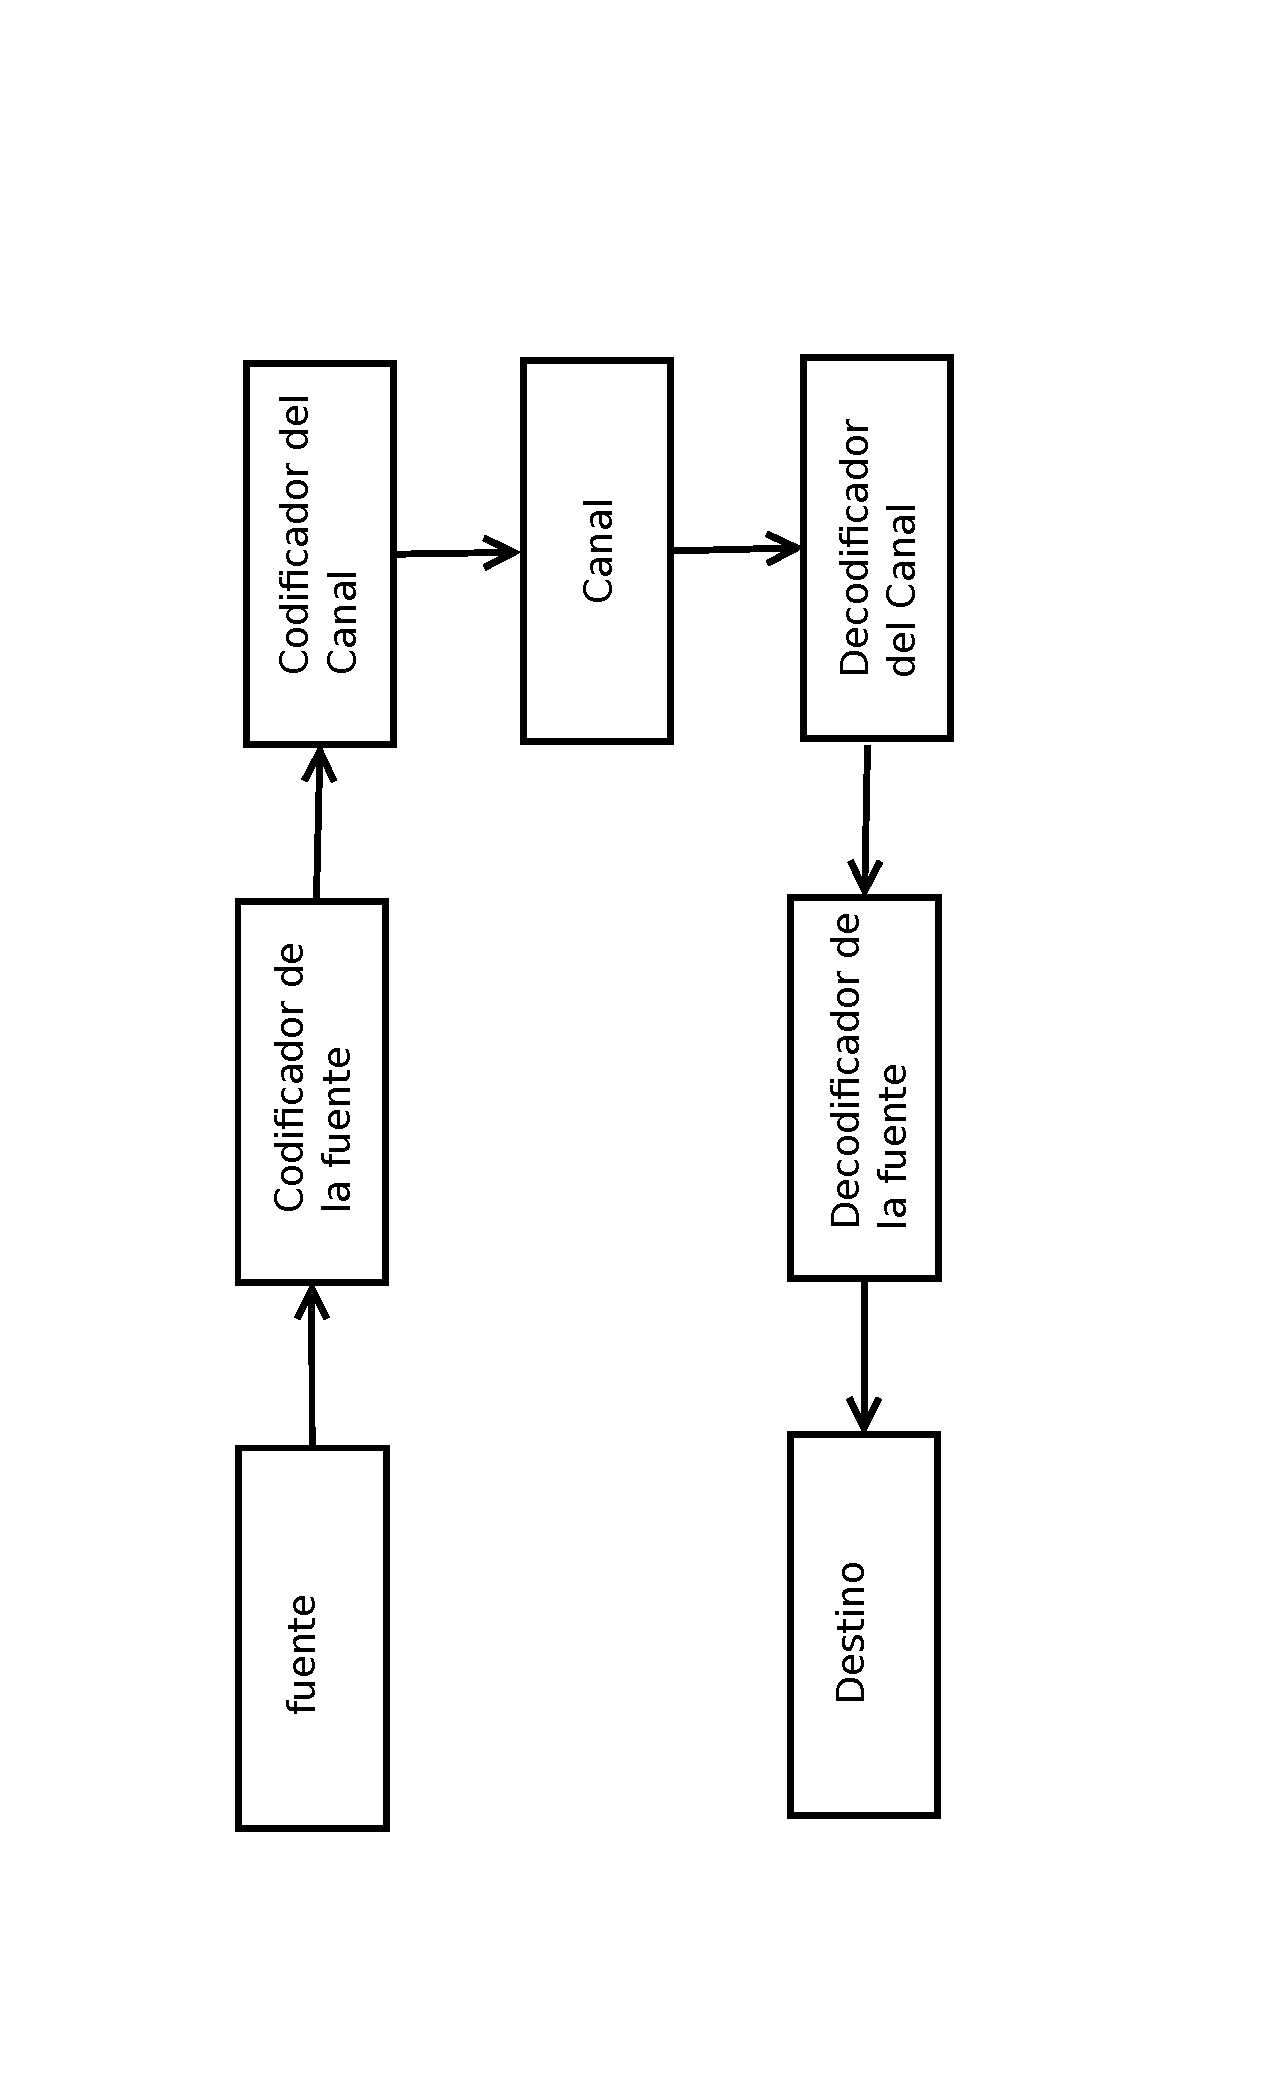
\includegraphics[angle=-90,width=0.7\linewidth]{Pictures/sistema.pdf}
\caption*{Fuente: Elaboración propia con software Dia.}
\label{fig:sistemaComunicacion}
\end{figure}
La codificación de la fuente tiene doble propósito. Primero, servir como traductor entre la salida de la fuente y la entrada al canal. Por ejemplo, si la información transmitida de la fuente al destino está en señal análoga y el canal espera recibir señal digital, se necesitará una conversión de análoga a digital en la fase de codificación y un convertidor de señal digital a análoga en la fase de decodificación. Como segunda función se podría requerir que el codificador de la fuente comprima la salida de la fuente para economizar en la longitud de la transmisión, eso significa que en el otro extremo, el decodificador de la fuente necesitará descomprimir la señal.

Algunas aplicaciones necesitan que el decodificador restaure la información para que sea idéntica a la original, en cuyo caso se dice que la compresión es \textbf{sin pérdidas}.

Otras aplicaciones, como la mayoría de transmisiones de audio e imágenes, permiten una diferencia controlada o distorsión entre la información original y la restaurada, así que esta posibilidad es usada para lograr mayor compresión. En este caso se dice que la compresión es \textbf{con pérdidas.}

Los canales no son perfectos debido a limitaciones físicas y de ingeniería, es decir, su salida puede diferir de su entrada debido al ruido o a defectos de fabricación.

Más aún, en algunos casos el diseño requiere que el formato de la información de salida del canal difiera del formato de entrada. Además hay aplicaciones tales como los medios de almacenamiento masivo magnético y óptico, donde no se permiten ciertos patrones en el flujo de bits a transmitir. Dado esto, el rol principal del codificador del canal, es superar estas limitaciones y hacer el canal tan transparente  como sea posible, tanto desde el punto de vista de la fuente como del destino. 

Es así como entran a participar los códigos. Los códigos fueron inventados para corregir errores en los canales de comunicación debido al ruido. Por ejemplo, supóngase que hay un cable telegráfico desde Ciudad de Guatemala hasta Ciudad de Panamá, mediante el cual se pueden transmitir unos y ceros. Usualmente cuando un cero es enviado se recibe un cero, pero ocasionalmente un cero puede ser recibido como un uno o un uno como un cero. Supóngase que en promedio, 1 de cada 100 símbolos se recibe de forma errónea, es decir, por cada símbolo hay una probabilidad $p=1/100$ de que ocurra un error en el canal. A esto se le llama un canal binario simétrico y se denota como BSC por sus siglas en inglés.
\begin{figure}
\centering
\caption{Canal Binario Simétrico}
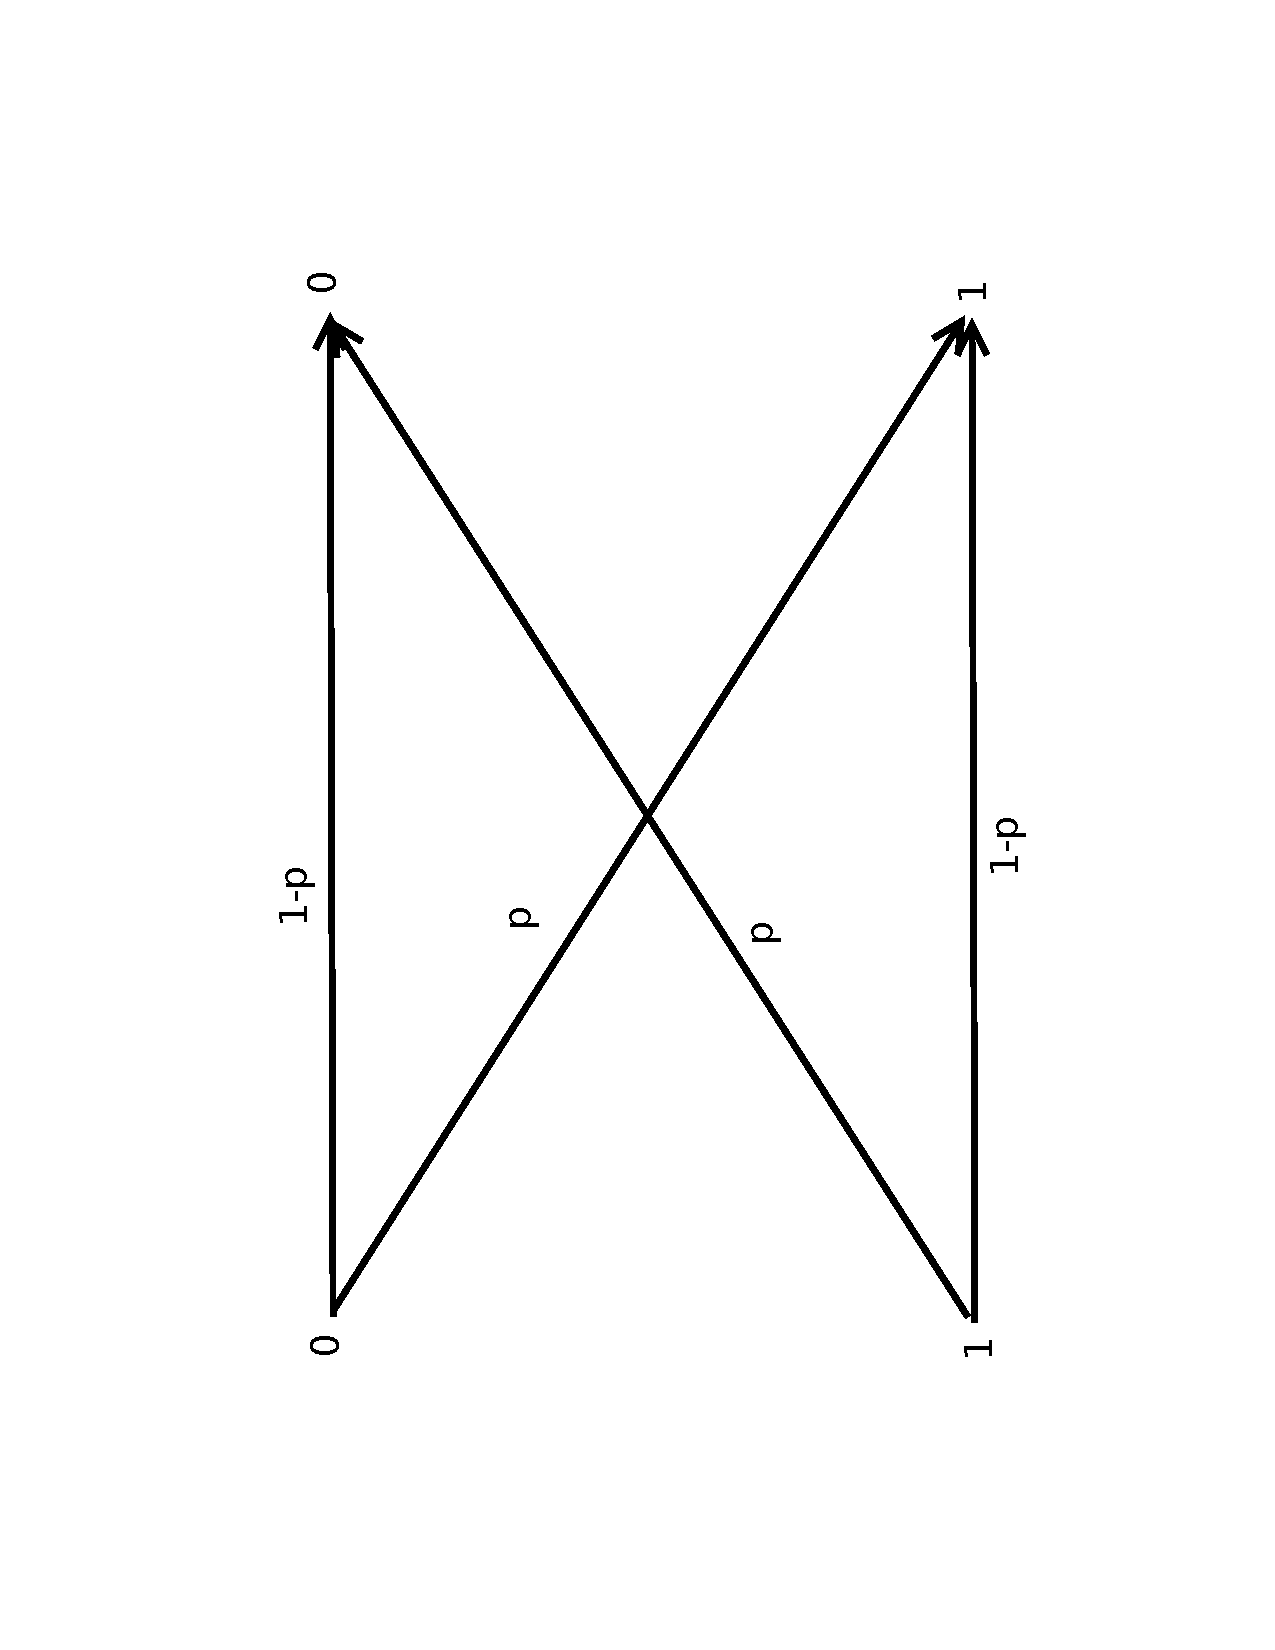
\includegraphics[angle=-90,width=0.6\linewidth]{Pictures/CBS.pdf}
\caption*{Fuente: Elaboración propia con software Dia.}
\label{fig:CBS}
\end{figure} 
Además supóngase que se enviarán muchos mensajes importantes por ese cable y se necesita enviarlos de manera rápida y segura. Los mensajes ya se encuentran escritos como cadenas de ceros y unos, producidos, quizás, por alguna computadora.

Se van a \textbf{codificar} estos mensajes para darles una protección en contra del ruido del canal. Un bloque de $k$ símbolos del mensaje $u = u_1\dots u_k,\ u_i = 0 \mbox{ o } 1$, será codificado como una \textbf{palabra-código} $x = x_1 \dots x_n, x_i = 0 \mbox{ o } 1$ donde $n \geq k$ (véase la figura \ref{fig:codificacion}). Estas palabra-códigos forman un código.
\begin{figure}
\caption{Proceso de Codificación}
\centering
% Graphic for TeX using PGF
% Title: /mnt/DataWin/Dropbox/Tesis/Tesis Actual/codi.dia
% Creator: Dia v0.97.2
% CreationDate: Wed Dec 11 21:23:59 2013
% For: hugo
% \usepackage{tikz}
% The following commands are not supported in PSTricks at present
% We define them conditionally, so when they are implemented,
% this pgf file will use them.
\ifx\du\undefined
  \newlength{\du}
\fi
\setlength{\du}{15\unitlength}
\begin{tikzpicture}
\pgftransformxscale{0.800000}
\pgftransformyscale{-0.700000}
\definecolor{dialinecolor}{rgb}{0.000000, 0.000000, 0.000000}
\pgfsetstrokecolor{dialinecolor}
\definecolor{dialinecolor}{rgb}{1.000000, 1.000000, 1.000000}
\pgfsetfillcolor{dialinecolor}
\pgfsetlinewidth{0.100000\du}
\pgfsetdash{}{0pt}
\pgfsetdash{}{0pt}
\pgfsetmiterjoin
\definecolor{dialinecolor}{rgb}{1.000000, 1.000000, 1.000000}
\pgfsetfillcolor{dialinecolor}

\definecolor{dialinecolor}{rgb}{0.000000, 0.000000, 0.000000}
\pgfsetstrokecolor{dialinecolor}
\draw (3.731981\du,6.945629\du)--(3.731981\du,13.482575\du)--(9.631981\du,13.482575\du)--(9.631981\du,6.945629\du)--cycle;
% setfont left to latex
\definecolor{dialinecolor}{rgb}{0.000000, 0.000000, 0.000000}
\pgfsetstrokecolor{dialinecolor}
\node[anchor=west] at (4.006981\du,9.767031\du){Fuente del };
% setfont left to latex
\definecolor{dialinecolor}{rgb}{0.000000, 0.000000, 0.000000}
\pgfsetstrokecolor{dialinecolor}
\node[anchor=west] at (4.006981\du,11.089242\du){mensaje};
\pgfsetlinewidth{0.100000\du}
\pgfsetdash{}{0pt}
\pgfsetdash{}{0pt}
\pgfsetmiterjoin
\definecolor{dialinecolor}{rgb}{1.000000, 1.000000, 1.000000}
\pgfsetfillcolor{dialinecolor}
\definecolor{dialinecolor}{rgb}{0.000000, 0.000000, 0.000000}
\pgfsetstrokecolor{dialinecolor}
\draw (13.386981\du,8.142031\du)--(13.386981\du,12.282031\du)--(21.636981\du,12.282031\du)--(21.636981\du,8.142031\du)--cycle;
% setfont left to latex
\definecolor{dialinecolor}{rgb}{0.000000, 0.000000, 0.000000}
\pgfsetstrokecolor{dialinecolor}
\node[anchor=west] at (14.561981\du,10.357031\du){Codificador};
\pgfsetlinewidth{0.100000\du}
\pgfsetdash{}{0pt}
\pgfsetdash{}{0pt}
\pgfsetbuttcap
{
\definecolor{dialinecolor}{rgb}{0.000000, 0.000000, 0.000000}
\pgfsetfillcolor{dialinecolor}
% was here!!!
\pgfsetarrowsstart{to}
\definecolor{dialinecolor}{rgb}{0.000000, 0.000000, 0.000000}
\pgfsetstrokecolor{dialinecolor}
\draw (13.386981\du,10.212031\du)--(9.631981\du,10.214102\du);
}
\pgfsetlinewidth{0.100000\du}
\pgfsetdash{}{0pt}
\pgfsetdash{}{0pt}
\pgfsetbuttcap
{
\definecolor{dialinecolor}{rgb}{0.000000, 0.000000, 0.000000}
\pgfsetfillcolor{dialinecolor}
% was here!!!
\pgfsetarrowsstart{to}
\definecolor{dialinecolor}{rgb}{0.000000, 0.000000, 0.000000}
\pgfsetstrokecolor{dialinecolor}
%line i am interested in
\draw (28.770935\du,10.256598\du)--(21.636981\du,10.212031\du);
}
% setfont left to latex
\definecolor{dialinecolor}{rgb}{0.000000, 0.000000, 0.000000}
\pgfsetstrokecolor{dialinecolor}
\node[anchor=west] at (9.331981\du,11.042031\du){Mensaje};
% setfont left to latex
\definecolor{dialinecolor}{rgb}{0.000000, 0.000000, 0.000000}
\pgfsetstrokecolor{dialinecolor}
\node[anchor=west] at (9.331981\du,11.842031\du){$u_1\dots u_k$};
% setfont left to latex
\definecolor{dialinecolor}{rgb}{0.000000, 0.000000, 0.000000}
\pgfsetstrokecolor{dialinecolor}
\node[anchor=west] at (21.381981\du,11.292031\du){Palabra-código};
% setfont left to latex
\definecolor{dialinecolor}{rgb}{0.000000, 0.000000, 0.000000}
\pgfsetstrokecolor{dialinecolor}
\node[anchor=west] at (22.881981\du,12.092031\du){$x_1\dots x_n$};
\pgfsetlinewidth{0.100000\du}
\pgfsetdash{}{0pt}
\pgfsetdash{}{0pt}
\pgfsetmiterjoin
\definecolor{dialinecolor}{rgb}{1.000000, 1.000000, 1.000000}
\pgfsetfillcolor{dialinecolor}
\definecolor{dialinecolor}{rgb}{0.000000, 0.000000, 0.000000}
\pgfsetstrokecolor{dialinecolor}
\draw (28.820292\du,7.014162\du)--(28.820292\du,13.551108\du)--(34.720292\du,13.551108\du)--(34.720292\du,7.014162\du)--cycle;
% setfont left to latex
\definecolor{dialinecolor}{rgb}{0.000000, 0.000000, 0.000000}
\pgfsetstrokecolor{dialinecolor}
\node[anchor=west] at (30.099923\du,10.484211\du){Canal};
% setfont left to latex
\definecolor{dialinecolor}{rgb}{0.000000, 0.000000, 0.000000}
\pgfsetstrokecolor{dialinecolor}
\node[anchor=west] at (30.168743\du,15.632869\du){Ruido};
\pgfsetlinewidth{0.100000\du}
\pgfsetdash{}{0pt}
\pgfsetdash{}{0pt}
\pgfsetbuttcap
{
\definecolor{dialinecolor}{rgb}{0.000000, 0.000000, 0.000000}
\pgfsetfillcolor{dialinecolor}
% was here!!!
\pgfsetarrowsstart{to}
\definecolor{dialinecolor}{rgb}{0.000000, 0.000000, 0.000000}
\pgfsetstrokecolor{dialinecolor}
\draw (31.770292\du,13.551108\du)--(31.802718\du,15.192715\du);
}
\end{tikzpicture}

\caption*{Fuente: Elaboración propia con software Dia y exportado a \TeX}
\label{fig:codificacion}
\end{figure}
La primera parte de la palabra-código consiste en el mensaje mismo: \[ x_1 = u_1,\ x_2 = u_2,\ \dots ,\ x_k = u_k, \] seguido de $n-k$ símbolos de comparación $x_{k+1}, \dots , x_n$. 
Los símbolos de comparación son elegidos de tal forma que las palabra-códigos satisfagan 
\[ H \begin{pmatrix}
x_1 \\ 
x_2 \\
\vdots \\
x_n
\end{pmatrix} = Hx^{t} = 0, \] donde la matriz $H$ de $(n-k)\times k$ es la matriz de comparación de paridad del código, dada por 
\begin{equation}\label{ecu:defCodigo}
H = [A \mid I_{n-k}],
\end{equation}  
donde $A$ es una matriz fija de $(n-k)\times k$ de ceros y unos e \[ I = \begin{pmatrix}
1 & 0 & \dots & 0 \\
0 & 1 & \dots & 0 \\
\vdots & \vdots & \ddots & \vdots \\
0 & 0 & \dots & 1
\end{pmatrix} \] es la matriz identidad de $(n-k) \times (n-k)$. La aritmética en la ecuación \ref{ecu:defCodigo} se hace en módulo 2, es decir que se está trabajando con el campo $\mathds{Z}_2$. 
\begin{ejemplo}
La matriz de comparación de paridad 
\[ H = \left(\begin{array}{ccc|ccc}
0 & 1 & 1 & 1 & 0 & 0 \\
1 & 0 & 1 & 0 & 1 & 0 \\
1 & 1 & 0 & 0 & 0 & 1
\end{array}\right) \] define un código con $k=3$ y $n=6$. Para este código 
\[ A = \begin{pmatrix}
0 & 1 & 1\\
1 & 0 & 1 \\
1 & 1 & 0
\end{pmatrix}.  \]
El mensaje $u_1u_2u_3$ es codificado en la palabra-código $x = x_1x_2x_3x_4x_5x_6$ que empieza con el propio mensaje:
\[ x_1 = u_1, x_2 = u_2, x_3 = u_3, \] seguido de tres símbolos de comparación $x_4x_5x_6$ tales que $Hx^t = 0$, es decir, se cumple
\begin{eqnarray}\label{ecu:comparacion}
x_2 + x_3 + x_4 = 0, \\
x_1 + x_3 + x_5 = 0, \\
x_1 + x_2 + x_6 = 0.
\end{eqnarray}
Si el mensaje es $u = 011$, entonces $x_1= 0,\  x_2 = 1, \ x_3 =1$ y los símbolos de comparación son
\begin{eqnarray*}
x_4 & = & 0 \\
x_5 &=& 1 \\
x_6 &=& 1
\end{eqnarray*}
por lo que la palabra-código es $x = 011011$.
\end{ejemplo}
Las ecuaciones \ref{ecu:comparacion} son llamadas ecuaciones de comparación de paridad del código. Las ecuaciones de paridad dicen que el cuarto, quinto y sexto símbolo siempre deben sumar cero módulo 2, es decir, su suma siempre es par. 

Es fácil notar que el número de palabra-códigos posibles para esta matriz es $2^3 = 8$. Estas son:
\[ \begin{array}{ccc}
000000 & 011011 & 110110 \\
001110 & 100011 & 111000 \\
010101 & 101101 & 
\end{array}. \]
En general en un código hay $2^k$ palabra-códigos, si el alfabeto es $\{0,1\}$.

Luego de haber visto de manera intuitiva un código lineal, se da la definición formal:
\begin{definicion}
Un código de bloques lineal sobre GF(q) de longitud $n$ y dimensión $k$, es un subespacio de $V_n(q)$ de dimensión $k$, donde $V_n(q)$ es un espacio vectorial de dimensión $n$ sobre GF(q). Se denota a este como \textbf{código lineal $(n,k)$}.
\end{definicion}
El término código de bloques se refiere al hecho que toda palabra-código tiene la misma longitud, es decir, es una $n\mbox{-upla}$. La palabra lineal se deriva del simple hecho que las palabra-códigos forman un subespacio. 
También existen los códigos de árbol, de los cuales los códigos de convolución son un caso especial. Dichos códigos no dividen el mensaje en bloques. En la práctica de la ingeniería estos códigos son bastante importantes, pero no se hablará de estos en este trabajo.
\begin{definicion}
La distancia de Hamming $d(u,v)$ entre dos $n\mbox{-uplas}$ $u$ y $v$ de $V_n(q)$ está definida como el número de coordenadas en el cual difieren. El peso de Hamming $\omega(u)$ de una $n\mbox{-upla } u \in V_n(q)$ es el número de coordenadas no nulas de $u$.
\end{definicion}
La mayor parte del trabajo en teoría de códigos se desarrolla en base a la distancia de Hamming. Otra métrica con la que también se trabaja es la de Lee.

Como se dijo anteriormente, en la transmisión de una palabra-código en algún canal se puede producir errores debido al ruido. Por error, se entiende que puede ocurrir un cambio en cualquiera de las coordenadas de la $n\mbox{-upla}$ trasmitida. Justamente el punto de codificar es que, bajo ciertas circunstancias, estos errores se pueden corregir.

\section{\quad Códigos Cíclicos} 

Ya que se ha hecho la presentación de los códigos lineales, se procede a estudiar una clase muy particular e importante de ellos; los códigos cíclicos.

\begin{definicion}
Un código es cíclico si es lineal y además todo desplazamiento cíclico de las coordenadas de una palabra-código es también una palabra-código. 
\end{definicion}
Los códigos cíclicos figuran entre los primeros que aparecieron para el uso práctico, estos eran implementados usando registros de desplazamientos. 
Para poder hacer un buen diseño de códigos es necesario conocer la estructura algebraica de los mismos. en esta sección se abordará la estructura algebraica de los códigos cíclicos.
El lector deberá notar que los códigos cíclicos no dependen de la linealidad de los mismos, de hecho, también existen los códigos cíclicos no lineales.

Resulta muy conveniente identificar a los códigos cíclicos con polinomios, esto es, a cada palabra-código
\[ a = (a_0, a_1, \dots , a_{n-1}) \in \mathds{F}^n \] se le asocia el polinomio \[ a(x) = a_0 + a_1x+ \cdots + a_{n-1}x^{n-1} \in \mathds{F}[x]_n .\] Si $c$ es una palabra-código del código $\mathcal{C}$, entonces $c(x)$ es su polinomio-código asociado. Con esta identificación, la palabra-código con corrimiento $\tilde{c}$ tiene el polinomio-código asociado \[ \tilde{c}(x) = c_{n-1} + c_0x + c_1x^2 + \cdots + c_{n-2}x^{n-2}. \] Así, es tentador pensar que $\tilde{c}(x) $ es casi igual al producto $xc(x)$. Más aún, 
\[ \tilde{c}(x) = xc(x) - c_{n-1}(x^n -1)  \] de donde se deduce que \[ \tilde{c}(x) = xc(x) (\mbox{mód } x^n-1) .\] Dicho de otra manera $\tilde{c}(x)$y $xc(x)$ son iguales en el anillo de polinomios $\mathds{F}[x]$ con multiplicación módulo $x^n-1$. Como se esta trabajando con códigos, según la definición $\mathds{F} = GF(q) $ y $GF(q)[x]$ es el anillo de polinomios sobre $GF(q)$ en la variable $x$. Entonces, por lo dicho en el párrafo anterior, resulta claro que hay un isomorfismo natural entre $GF(q)[x]/(x^n-1)$ y los polinomios de grado menor que $n$ con multiplicación definida módulo $x^n-1$. Se denota al anillo $GF(q)[x]/(x^n-1)$ como $A_n$. Es claro que $A_n$ es también un álgebra sobre $GF(q)$. Más aún, si $C_n = \langle x \rangle,\ x^n =1$, es un grupo cíclico de orden $n$, es evidente que existe un isomorfismo entre $GF(q)C_n$ y $GF(q)[x]/(x^n-1) = A_n$, donde se ha utilizado el símbolo $x$ para ambas álgebras con el único propósito de hacer énfasis en esta identificación.
Lo anterior quiere decir que $A_n \simeq GF(q)C_n$, pero $GF(q)C_n$ es un grupo-álgebra, con lo cual se ha demostrado que los códigos cíclicos son un grupo-álgebra y por lo tanto su estructura algebraica está plenamente identificada. Además se tiene el siguiente teorema:
\begin{teorema}
Un código $(n,k) \ \mathcal{C}$ sobre $GF(q)$ es lineal si y sólo si dicho código es un ideal de $A_n$.
\end{teorema}
\begin{proof}
Sea $\mathcal{C}$ un ideal de $A_n$. Es claro que $\mathcal{C}$ es un subespacio de $A_n$ como espacio vectorial, por lo que solamente falta verificar que es un subespacio cíclico, lo cual se sigue del hecho que $\mathcal{C}$ es ideal y por lo tanto cerrado bajo multiplicación por $x$.
Para el converso, supóngase que $\mathcal{C}$ es un subespacio cíclico, eso quiere decir que es cerrado bajo la suma y el producto por $x$ y por lo tanto es cerrado bajo el producto de cualquier elemento de $A_n$, entonces $\mathcal{C}$ es un ideal.
\end{proof}
Como el lector podrá notar, el estudio de códigos lineales, se reduce a estudiar los ideales de $A_n$, que es un grupo-álgebra. Para ello será provechoso conocer cuando $A_n$ es semisimple o no, tarea que se realizó en el capítulo 3. 






%----------------Inicio del apartado Final de la tesis ------------------------------
% Modificación para tabla de contenidos
%\addtocontents{toc}{\protect\addvspace{+.8cm}}
     %En el apartado final, las páginas son numeradas como en apartado principal (la numeración continúa) 
     %pero los capítulos no son numerados. 
     \backmatter     		
     % Modificación para tabla de contenidos
     \addtocontents{toc}{\protect\addvspace{1.8em}}
     \chapter{CONCLUSIONES}


\begin{finalList}
\item Para el estudio de los grupo-anillos es importante conocer la estructura de los grupos abelianos y hamiltonianos, así como la teoría de módulos y el teorema de Wedderburn-Artin.
\item Las condiciones necesarias y suficientes para que un grupo-anillo sea semisimple, vienen dadas por el teorema de Maschke.
\item Toda representación de un anillo conmutativo sobre un grupo dado, corresponde a un módulo del grupo-anillo correspondiente.
\item En general no es fácil encontrar unidades no triviales en grupo-anillos, pero es posible construir algunas usando elementos idempotentes.
\item Las grupo-álgebras dan estructura matemática a los códigos correctores conocidos como cíclicos. 
\item Cuando la característica del campo no divide al orden del grupo el estudio de los códigos cíclicos se reduce a estudiar los ideales de grupo-álgebras generadas por elementos idempotentes.
\end{finalList}

     \chapter{RECOMENDACIONES}



\begin{finalList}

\item Usar el primer capítulo como guía de temas para el desarrollo de un curso de álgebra moderna de pregrado. 

\item Para el estudio de los códigos cíclicos, se puede utilizar los resultados del capítulo 2, en especial los de las secciones 2.3 y 2.4.

\item Estudiar la teoría de códigos correctores desde el punto de vista algebraico, permitiendo así dictaminar la capacidad correctora de los mismos.

\item Para la lectura de los capítulos 2 y 3 es importante tener conocimientos previos de teoría de grupos y anillos. 

\item Implementar el estudio de teoría de módulos en el curso de álgebra 2 de la licenciatura en Matemática Aplicada de la USAC.
\end{finalList}

     \begin{thebibliography}{99}
    \addcontentsline{toc}{chapter}{BIBLIOGRAFÍA}
    % LETRA B
    \bibitem{bib:libroLosGrandes} BELL, Eric. \textit{Los grandes matemáticos.} Argentina: Editorial Losada, 1948.
    \bibitem{bib:codeBook} BLAKE, Ian.\textit{The mathematical theory of coding}. Estados Unidos: Academic Press Inc, 1975.
    \bibitem{bib:burnside} BURNSIDE, William. \textit{The theory of Groups of Finite Order}. 	2da ed. Cambridge: Cambridge University Press, 1911.
        
    
    %LETRA C
     \bibitem{bib:Cauchy} CAUCHY, Augustin-Louis. Oeuvres complètes. 1era ed. Cambridge: Cambridge University Press, 2009.
     
     %LETRA D
     \bibitem{bib:Deskins} DESKINS, Eugene. ``Finite abelian groups with isomorphic group algebras". \textit{Duke Mathematical Journal}. 1956, vol 23, núm. 1, p. 35-40.
     
     %LETRA F
      \bibitem{bib:solubilidad} FEIT, Walter, et al.  ``The solvability of groups of odd order". \textit{Pacific J. Math}. 1963, vol 13, núm 3, p. 775-1029.
      
    %LETRA G
    \bibitem{bib:grupsfact}  GOLDSHMIDT, David. ``A group theoretic proof of the $p^aq^b$ theorem for odd primes". \textit{Mathematische Zeitschrift}. 1970, vol 113, núm. 5, p. 373-375.
    
    %LETRA H
     \bibitem{bib:historia} HAWKINS, Thomas. ``The origins of the Theory of Group Characters". \textit{Archive for History of Exact Sciences}. 1971, vol 7, núm. 2, p. 142-170.
    \bibitem{bib:herstein} HERSTEIN, Nathain. \textit{Topics in Algebra}. 2da ed.  New York: Macmillah, 1986 . 381 p. 
    
   %LETRA I
 	\bibitem{bib:Connell} IAN, Connell. ``On the group ring". \textit{Canad. J. Math}. 1963, vol 15, núm 1, p. 650-685.
 	
   \bibitem{bib:AlgebraPostGrado}ISAACS, Martin. \textit{Algebra: a graduate course}. Estados Unidos: Editorial Pacific Grove, 1940.   
   
   %LETRA J
   \bibitem{bib:Jeanings} JENNINGS, Arthur. ``The structure of the group ring of a p-group over a modular field". \textit{Transactions of The American Mathematical Society}. 1941, vol. 50, núm 1, p. 175-185.
   
   
   %LETRA L    
    \bibitem{bib:lang}LANG, Serge. \textit{Linear Algebra}. 3ra ed. Nueva York: Springer-Verlag, 2004. 308 p.
    
    %LETRA M
    \bibitem{bib:moser} MOSER, Claude. ``Representation de -1 comme somme de carres dans un corps cyclotomique quelconque". \textit{Journal of Number Theory}. 1973, vol 5, núm. 2, p. 138-141.
    
    %LETRA P
    \bibitem{bib:passman} PASSMAN, Donald. \textit{The algebraic structure of group rings}. New York: Wiley-Interscience, 1977. 550 p.
    \bibitem{bib:PerlisWalker} PERLIS, Sam; WALKER, Gordon. ``Abelian group algebras of finite order". \textit{Transactions of The American Mathematical Society}. 1950, vol 68, núm 3, p. 420-426.
    \bibitem{bib:main} POLCINO, César; SEHGAL, Sudarshan. \textit{An introduction to group rings}.  Dordrecht: Kluwer Academic Publishers, 2002. 371 p.
    
    %LETRA S
    \bibitem{bib:libroGuti} STEWART, Ian. \textit{De aquí al infinito -- Las matemáticas de hoy.} España: Editorial Crítica, 1998.
    \bibitem{bib:Sehgal} SUDARSHAN, Sehgal.  \textit{Topics in Group Rings}.New York: Marcel Dekker, 1978. 233 p. 
    
    
    %LETRA Z
    
	\bibitem{bib:groupBook} ZASSENHAUS, Hans. \textit{The theory of groups}. Estados Unidos: Chelsea publishing company, 1937.
	
		
		
\end{thebibliography}

     
\end{document}




